\PassOptionsToPackage{table, dvipsnames}{xcolor}
\documentclass[a4paper, oneside,12pt]{toptesi}
\usepackage[T1]{fontenc}
\usepackage[utf8]{inputenc}
\usepackage[italian]{babel}
\usepackage{natbib} 
\bibliographystyle{plain}
\usepackage{graphicx}
\usepackage{tikz}
\usetikzlibrary{positioning}
\usepackage{pgfplots}
\usepackage[newfloat]{minted}
\usepackage[font=small,skip=1pt]{caption}
\usepackage{minted}
\usepackage{subcaption}
\pgfplotsset{compat=1.18}
\usepackage{lscape}
\usepackage{adjustbox}
\usepackage{graphicx}
\usepackage{wrapfig}
\usepackage{microtype}
\usepackage{tocloft}
\usepackage{xcolor}
\usepackage{amsmath}

\sloppy

\SetupFloatingEnvironment{listing}{name=Codice}


\usepackage{minted}
\usemintedstyle{monokai}
\definecolor{bg}{RGB}{40, 44, 52}



% ===== Define abstract environment =====
\newcommand{\prefacename}{Preface}
\newenvironment{preface}{
    \vspace*{\stretch{1}}
    {\noindent \bfseries \Huge \prefacename}
    \begin{center}
        % \phantomsection \addcontentsline{toc}{chapter}{\prefacename} % enable this if you want to put the preface in the table of contents
        \thispagestyle{plain}
    \end{center}%
}
{\vspace*{\stretch{1}}}


\newcommand{\walter}[1]{\textcolor{red}{{\bf [Walter: }{#1}{\bf ]}}}

\usepackage{hyperref}

\hypersetup{
    colorlinks = true,
    allcolors=black
}

%%% workaround for listing
% save the current meaning of \listing
\let\savedlisting\listing
% at the right spot, restore the meaning
\AtBeginDocument{\let\listing\savedlisting}
%%% end of workaround


\def\dept{Dipartimento di Informatica}
\def\course{Corso di Laurea in Informatica}
\def\title{Analisi espressioni facciali in contesto di e-learning}
\def\author{Alessandro Carella}
\def\beforeprof{Professore}
\def\prof{Prof. Stefano Ferilli\newline\newline Prof. Berardina Nadja De Carolis}
\def\beforeRelatore {Relatrice}
\def\beforetitle{Tesi di Laurea in}
\def\subject{Informatica}
\def\annoacc{2022 - 2023}
\def\beforecandidate{Laureando}
\def\beforeannoacc{Anno Accademico}

\makeatletter
\def\cleardoublepage{\clearpage\if@twoside \ifodd\c@page\else
    \hbox{}
    \vspace*{\fill}
    \vspace{\fill}
    \thispagestyle{empty}
    \newpage
    \if@twocolumn\hbox{}\newpage\fi\fi\fi}
\makeatother


\begin{document}

%\maketitle


\begin{titlepage}
	\begin{tikzpicture}[remember picture,overlay]
		\centering
			\node[yshift=-6 cm] (logo) at (current page.north) {
\includegraphics[width=0.35\linewidth]{images/logo uniba.png}};
			\node[text width=50em,yshift=0.25cm, align = center, below = of logo](uniba){\bfseries \Large Università degli Studi di Bari Aldo Moro};
			\node[text width=40em, align = center, yshift=.55cm,below = of uniba](course){\normalsize \dept \\
% 
				\normalsize \textbf{\course}};
		\node[text width=35em,align = center,  yshift=1.2cm,below = of course](line){\par\noindent\rule{\textwidth}{0.4pt}};
		\node[text width=40em, align = center, yshift=.55cm,below = of line](lia){\beforetitle\xspace \subject};
		\node[text width=40em, align = center, yshift=-0.5cm,below = of lia](title){\bfseries \fontsize{21pt}{20pt}\selectfont \title\par};
	\node[text width=35em, align = left, yshift=-0.75cm,below = of title](supervisor){\large \beforeprof \\ \textbf{\prof}};
	\node[text width=35em, align = left, yshift=-1.9cm,below = of title](supervisor){\large \beforeRelatore \\ \textbf{\relatore}};
		\node[text width=35em, align = right, yshift=0cm,below = of supervisor](candidate){\large \beforecandidate\\ \textbf{\author}};
		\node[text width=35em,align = center,  yshift= 0cm,below = of candidate](line2){\par\noindent\rule{\textwidth}{0.4pt}};
		\node[text width=50em, align = center, yshift=0.5cm,below = of line2](year){\beforeannoacc\xspace \annoacc};
	\end{tikzpicture}
\end{titlepage}


\cleardoublepage
% Dedication

\thispagestyle{empty}
%\refstepcounter{dummy}

\pdfbookmark[1]{Dedication}{Dedication} % Bookmark name visible in a PDF viewer

\vspace*{3cm}

%\begin{center}
%\emph{Ohana} means family. \\
%Family means nobody gets left behind, or forgotten. \\ \medskip
%--- Lilo \& Stitch    
%\end{center}

\medskip

\begin{flushright}
\textit{Dedication, \\ continuing dedication.} \\ \smallskip
%%1939\,--\,2005
\end{flushright}

\cleardoublepage

\pagenumbering{roman}

\chapter*{Abstract}

Il testo di tesi mira a identificare gli stati d’animo delle persone attraverso l’analisi di immagini o video che le riprendono.

Come attestato da diversi studi, gli stati d’animo incidono notevolmente sulle performance individuali, ed è per questo utile avere delle informazioni a riguardo col fine di rimodulare le attività e migliorare l’esperienza del singolo.

Lo studio trova applicazione sia in contesti di e-learning che di lavoro, o in qualsiasi altro contesto dove sia possibile ottenere delle riprese.

Un esempio pratico di un applicativo che usufruisce dei risultati del mio studio è l’utilizzo di questo, da parte di un docente, durante una lezione; l’insegnante, avendo cognizione dello stato d’animo dei suoi studenti, ha la possibilità di adattare lo stile di insegnamento e rendere più agevole la fruizione della lezione per i suoi alunni.

\cleardoublepage

\tableofcontents

\cleardoublepage


\pagenumbering{arabic}
\setcounter{page}{1}
\begin{preface}
    “The test of successful education is not the amount of knowledge that pupils take away from school, but their appetite to know and their capacity to learn.” 
    -Sir Richard Livingstone 1941. \cite{Livingstone}
    
    La ricerca moderna, conseguentemente al fenomeno della pandemia da Covid-19, ha riservato attenzione sempre maggiore al tema della fruizione di contenuti, sia dal punto di vista dell’intrattenimento che dal punto di vista della produttività individuale.
    
    La pandemia ha quindi consentito alla ricerca l’impiego di strumenti impattanti in questo campo, in quanto ormai possibile osservare e quindi analizzare, le attitudini comportamentali del singolo, per migliorare l’esperienza di utilizzo dei prodotti software.
    
    Effettuando diverse ricerche a riguardo ho potuto constatare che la maggior parte degli studi precedentemente effettuati si concentra sull’analisi delle emozioni che vengono categorizzate come primarie dal sistema FACS (Facial Action Coding System) \cite{FacialCodingContinMonitor}:
    \begin{itemize}
        \item Happiness,
        \item Anger,
        \item Sadness,
        \item Disgust,
        \item Fear,
        \item Neutral
    \end{itemize}
    
    Di contro argomenti quali gli stati d’animo (o mood), che influenzano l’engagement degli studenti durante l’apprendimento, sono stati ampiamente trascurati.
    
    Diversi studi hanno dimostrato che gli stati d’animo positivi sono direttamente collegati al pensiero creativo e alla capacità dell’individuo di riflettere su ciò che sta compiendo, indi una maggiore agevolezza e beneficio nell’apprendimento che ne consegue; diversamente gli stati d’animo negativi sono correlati ad una maggiore difficoltà di esercitare queste caratteristiche portando ad un minore rendimento relativamente a questo ambito.
    
    Per quanto le emozioni primarie forniscano sicuramente un indicatore dello stato d’animo, e del conseguente miglioramento dell’esperienza di apprendimento o di lavoro, non sono però generalmente manifestate in modo esplicito, soprattutto per quanto concerne le espressioni facciali, in contesti di ufficio e studio.
    
    Coerentemente si è ritenuto fondamentale concentrare lo studio sulle espressioni facciali e i mood più frequenti all’interno di questi ambienti.
    
    Nei prossimi paragrafi analizzerò degli studi riguardanti sia l’analisi degli stati d’animo e i relativi procedimenti adoperati per effettuarli, che vari studi inerenti al FACS (Facial Action Coding System).
    
    \begin{figure}
        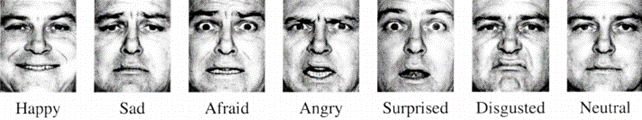
\includegraphics[width=1\linewidth]{images/1.png}
        \caption{Emozioni nel sistema FACS}
    \end{figure}
\end{preface}
\chapter{Stato dell'arte}

\section{Studi sull’engagement all’interno degli ambienti di studio}
Gli studi ritrovati che effettuano quest’analisi o trattano un argomento simile o tangente sono:
\subsection{Recognizing Cognitive Emotions in E-Learning Environment}
In questo studio (\cite{RecoCognEmoELearnEnv}) gli stati di d’animo che vengono classificati dal loro sistema sono i seguenti:
\begin{itemize}
    \item Entusiasmo,
    \item Interesse,
    \item Sorpresa,
    \item Noia,
    \item Perplessità,
    \item Frustrazione,
    \item Neutrale
\end{itemize}

Viene riportato che gli stati d’animo positivi (entusiasmo, interesse e sorpresa) sono spesso associati al raggiungimento del “flow state” da parte dello studente.

Più il singolo soggetto mantiene costante un mood positivo, tanto più permarrà in questo flow state, con esito un apprendimento più veloce ed efficace.

Il raggiungimento di questo mood è stato inoltre connesso alla capacità dei singoli studenti di percepirsi come autosufficienti nel corso dell’attività di studio.

Questa percezione di sé stessi deriva dall’attitudine dello studente nel riuscire ad essere in controllo della sua personale situazione di studio, rispecchiandosi nella sua abilità di:
\begin{itemize}
    \item pianificare,
    \item controllare,
    \item dirigere
\end{itemize}
l’attività di apprendimento.

È quindi necessario che gli studenti maturino una certa dimestichezza nello studio, e che vengano dunque supportati in vista dell’approccio ai problemi che vengono da loro riconosciuti in quanto difficili.

Naturalmente un sistema che permette di “leggere” con precisione lo stato d’animo di uno studente/studentessa o persino di un’intera classe, e quindi capire se questi si trovino nello stato di flow che possa permettere una migliore performance, è uno strumento utile per qualsiasi insegnante.

Un esempio circoscritto all’ambiente di lavoro potrebbe invece essere un’analisi del lavoratore nello svolgimento di un task e la possibilità, da parte di un capo progetto o di un tutor, di poter intervenire esclusivamente nel momento in cui il suo subordinato stia riscontrando dei problemi; in tal modo è permessa al dipendente una crescita professionale adeguata e non seguita al 100\%, così da sfruttare al meglio l’impiego del tempo del tutor.

\subsection {The faces of Engagement: Automatic Recognition of Student Engagement from Facial Expression}

In \cite{FacesOfEngagement}, gli stati d’animo organizzati in scala da meno attento/a a più attento/a, sono:
\begin{itemize}
    \item Not engaged at all (Non coinvolto: che guarda da un’altra parte, che sta ovviamente non pensando al compito, occhi completamente chiusi)
    \item Nominally engaged (Formalmente coinvolto: occhi appena aperti, chiaramente non attento/a al task che sta svolgendo)
    \item Engaged in task (Coinvolto nel task: requisito che non richiede un’ammonizione per la progressione del task)
    \item Very engaged (Altamente coinvolto: lo/a studente/tessa potrebbe essere elogiato/a per il suo livello di coinvolgimento)
    \item Clip/frame non chiaro (l’immagine analizzata non contiene una persona o comunque non è possibile effettuare un’identificazione)
\end{itemize}

Lo studio si concentra sull’effettuare una stima dell’engagement degli studenti. 

È stato inizialmente sviluppato un metodo per rilevare automaticamente l’engagement, si è poi indagato su quali segnali siano utilizzati nel riconoscimento automatico effettuato dal computer per poi individuare quali strumenti vengano adoperati dagli insegnanti per risolvere il medesimo task.

Infine si è investigato sulla correlazione effettiva fra i risultati di queste analisi e la qualità delle performance degli studenti.

\begin{figure}
    \begin{center}    
        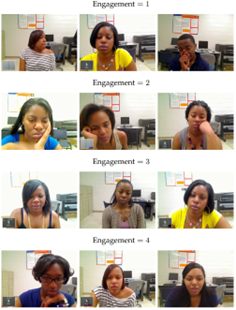
\includegraphics[width=0.4\linewidth]{images/2.png}
        \caption{Esempio campioni dal dataset dello studio}
    \end{center}
\end{figure}

\subsection{Facial coding as a mean to enable continuous monitoring of student’s behaviour in e-Learning }

Il paper \cite{FacialCodingContinMonitor} si focalizza sul tracciamento continuo degli studenti, sia per quanto riguarda una vera e propria identificazione degli stessi attraverso il riconoscimento facciale, sia per calcolarne il livello di attenzione ed eventualmente stimarne le emozioni provate durante i corsi MOOCs (Massive Open Online Courses).

Per dirigere l’analisi del livello di attenzione, si è ricorso all’uso della libreria esterna Dlib, la quale consente di creare una mappatura delle caratteristiche facciali dello/a studente; per giunta, la piattaforma include anche un gaze tracker che lascia prevedere la direzione dello sguardo degli studenti durante lo svolgimento del corso.

Questi tre aspetti vengono successivamente congiunti al fine di creare un applicativo web per l’apprendimento, attraverso il quale, alla fine di ogni lezione, è possibile visionare in quale percentuale della durata del corso le persone hanno adempito alle metriche citate nell'immagine \ref{fig:image32}.

\begin{figure}
    \begin{center}    
        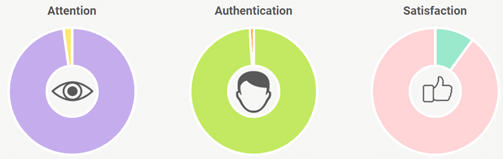
\includegraphics[width=1\linewidth]{images/3.png}
        \caption{Esempio di output del programma}
        \label{fig:image32}
    \end{center}
\end{figure}
 
\subsection{Prediction and Localization of student engagement in the wild}

Lo studio \cite{PredLocStudEngagInTheWild}, a differenza di altri, ha come premessa l’utilizzo delle immagini raccolte in ambienti non controllati per la creazione del modello che andrà successivamente ad effettuare la predizione per i nuovi campioni.

Per ambienti controllati, si intende setup di acquisizione dei video e delle immagini grazie ai quali non è possibile riscontrare problemi, quali scarsa illuminazione, occlusione ambientale, etc…

Per attuare ciò, sono stati sottoposti ad analisi molti studi precedentemente effettuati, per convenire al raccoglimento di campioni attraverso la fruizione, da parte dei soggetti, di video educazionali, categorizzando poi i vari video ed immagini ottenute in una scala, con valore da 0 a 3:
\begin{itemize}
    \item 0 \textrightarrow per niente interessato (il soggetto non sembra interessato e guarda spesso al di fuori dello schermo)
    \item 1 \textrightarrow poco interesse (il soggetto apre a malapena gli occhi, si muove in modo irrequieto sulla sedia)
    \item 2 \textrightarrow interessato/a al contenuto (sembra che al soggetto il contenuto riprodotto risulti interessante ed esso interagisce con questo)
    \item 3 \textrightarrow altamente interessato/a (il soggetto ha “gli occhi attaccati allo schermo” e risulta concentrato/a)
\end{itemize}


Hanno poi sfruttato un framework che esegue il riconoscimento dell’engagement e della localizzazione degli studenti.
\begin{itemize}
    \item Inizialmente vengono identificate la faccia e dei punti di riferimento all’interno di queste in ognuno dei frame analizzati 
    \item Procedendo, i video vengono suddivisi in segmenti più piccoli e le feature vengono estratte, “effettuando una media” dei risultati di ognuno dei frame.
    \item Si passa poi alla sequenza di frame successiva per effettuare la stessa analisi.
    \item Una volta raccolti tutti i dati, questi vengono elaborati per calcolarne l’engagement e la localizzazione attraverso la deep MIL network, impiegando la media e la top-k pooling per calcolarne la regressione.
\end{itemize}


\begin{figure}
    \begin{center}    
        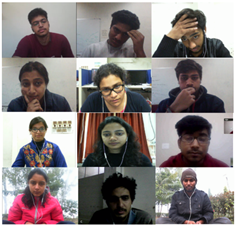
\includegraphics[width=0.8\linewidth]{images/4.png}
        \caption{Esempio di campioni dal dataset utilizzato in \cite{PredLocStudEngagInTheWild}}
    \end{center}
\end{figure}


\section{Studi sul riconoscimento delle emozioni FACS per scelta del modello da utilizzare}
Essendo l’ammontare di studi che trattano l’analisi delle emozioni FACS maggiore rispetto a quelle che cercano di creare sistemi di riconoscimento automatico per gli stati d’animo, i quali possono direttamente aiutare a identificare i problemi nell’apprendimento delle conoscenze, ho ritenuto opportuno studiare e selezionare fra i modelli da questi proposti per l’elaborazione delle informazioni per il mio caso di studio.

Il paper con i migliori risultati che ho trovato è stato \cite{FaceExpreRecoImgSeqTwoFoldRandomForestClass}, in questo studio viene utilizzata una random forest a due livelli:
\begin{itemize}
    \item il primo livello è utilizzato per determinare le Action Units nelle sequenze di espressioni che vengono analizzate
    \item il secondo livello invece prende in input le Action Units estratte, ed effettua la classificazione delle espressioni finali
\end{itemize}

Il modello riesce ad ottenere una media di riconoscimento del 100\% per le Action Units e del 96.38\% per le espressioni facciali (emozioni) che risulta essere migliore degli studi successivamente riportati.

Prima ancora di arrivare al primo livello della random forest viene utilizzato il modello AAM che identifica i punti di riferimento sulla faccia del soggetto ripreso nel video analizzato (o nella sequenza di immagini analizzate) per poi ricorrere all’utilizzo del Lucas-Kanade optical flow tracker col fine di tracciare i punti di riferimento nei frame successivi.

Viene poi calcolato il vettore di spostamento fra i punti di riferimento trovati sul primo frame, dove il soggetto si presenta con un’espressione neutrale, e i punti di riferimento trovati nel frame finale dove l’espressione facciale è al suo picco espressivo. 
Questo vettore di spostamento viene utilizzato nel primo layer della random forest per l’estrazione delle Action Units.

Le espressioni facciali sono processi dinamici, conseguenza dell'attività muscolare di varie parti del volto:
\begin{itemize}
    \item fronte,
    \item occhi,
    \item naso,
    \item bocca,
    \item mascella,
    \item contorno
\end{itemize}

Le caratteristiche dinamiche possono essere rappresentate dalla differenza tra i vettori estratti dai fotogrammi. 

Le sei espressioni facciali di base:
\begin{itemize}
    \item felicità,
    \item tristezza,
    \item rabbia,
    \item disgusto,
    \item paura,
    \item sorpresa
\end{itemize}
possono essere descritte utilizzando le AUs, codificate in base ai coinvolgimenti muscolari facciali.

Il processo di estrazione delle caratteristiche di movimento di un’espressione facciale è illustrato nella figura \ref{fig:image1}.
\begin{figure}
    \begin{center}    
        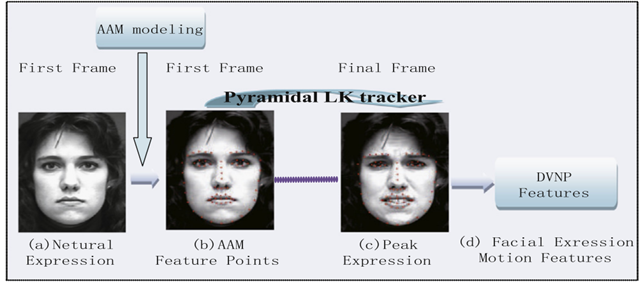
\includegraphics[width=1\linewidth]{images/14.png}
        \caption{Processo di estrazione dinamica delle feature delle espressioni facciali}
        \label{fig:image1}
    \end{center}
\end{figure}

Random Forest è un algoritmo di machine learning che combina degli alberi decisionali, all’interno dei quali ognuno di questi dipende dai valori di un vettore casuale campionato in modo indipendente e con la medesima distribuzione.

Questo algoritmo ha la capacità di gestire grandi spazi di caratteristiche grazie a due fonti di casualità, ovvero input e feature casuali, che lo rendono robusto. 

Random forest è da considerarsi affidabile per l'estimazione della posa, la rilevazione di oggetti e altre aree della computer vision grazie alla sua bassa complessità di calcolo, agevole implementazione, accuratezza nella classificazione e capacità di gestire grandi set di dati di addestramento. 

L’algoritmo è costituito da un gran numero di alberi decisionali, dove ciascuno viene costruito ricorsivamente assegnando un test binario ad ogni nodo, non foglia, in base ai samples di formazione. 

Per la classificazione combina i risultati degli alberi decisionali per fornire come risultato la classe più popolare. 

Questo algoritmo ha la capacità di gestire errori di bilanciamento nella popolazione delle classi in dati sbilanciati.

Per validare i risultati, i ricercatori hanno condotto degli esperimenti sui datasets Cohn-Kanade \cite{CohnKanadeDatabase} e Oulu-CAISA VIS \cite{OuluCasia} servendosi solo delle sequenze di immagini contenti una vista frontale o girata a 30 gradi dei soggetti.
Nel primo dataset sono categorizzate 7 espressioni (anger, contempt, disgust, fear, happy, sadness and surprise), con soggetti di età compresa fra i 18 e i 50 anni.

Il secondo dataset contiene samples ripresi in diverse condizioni di luce; nonostante ciò, sono state incluse solo le immagini con condizioni di illuminazione favorevoli (luce forte o buona illuminazione).

In entrambi i dataset, i video (e/o sequenze di immagini) riprendono delle persone che, in principio, mostrano un’espressione neutrale e, al termine, le espressioni che più esaltano l’emozione relativa al tag del video.

Nella fase finale del metodo proposto viene utilizzato l’ultimo layer della random forest per identificare l'etichetta finale dell'espressione facciale in base ai risultati della rilevazione delle AUs. 

Tale metodo viene messo a confronto con una rete bayesiana; questo modello predittivo ottiene un tasso di riconoscimento delle caratteristiche facciali dell’86,3\%. 

Il metodo proposto dal paper, basato sulle AUs, può invece incrementare il tasso di riconoscimento medio all’89,37\%. 

I risultati riportati nella tabella dell’immagine \ref{fig:image2} raffigurano il tasso di riconoscimento per la rilevazione dell'espressione facciale basata sulle AUs utilizzando il random forest. 
\begin{figure}
    \begin{center}    
        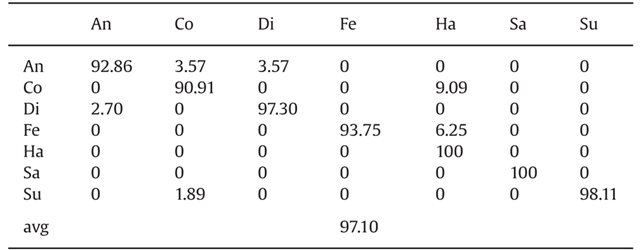
\includegraphics[width=0.7\linewidth]{images/15.png}
        \caption{Matrice di confusione del riconoscimento delle espressioni basato su Action Units usando Random Forest}
        \label{fig:image2}
    \end{center}
\end{figure}

Confrontando i risultati della Tabella riportata nell’immagine \ref{fig:image3}, dove sono raffigurati i tassi di riconoscimento della rete bayesiana, le prestazioni migliorano significativamente. 
\begin{figure}
    \begin{center}    
        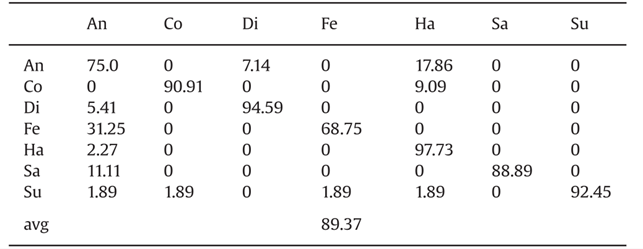
\includegraphics[width=0.7\linewidth]{images/16.png}
        \caption{Matrice di confusione del riconoscimento delle espressioni basato su Action Units usando Rete Bayesiana}
        \label{fig:image3}
    \end{center}
\end{figure}

Il classificatore con rete bayesiana ha un tasso di riconoscimento basso per le emozioni di tristezza e paura (rispettivamente 68,75\% e 88,89\%), mentre il random forest migliora queste prestazioni al 93,75\% e al 100\%.

Una possibile spiegazione è che la tristezza e la paura sono di solito poco evidenti e possono essere facilmente confuse con altre emozioni; tuttavia, il random forest ha maggiore capacità discriminativa e può trovare la differenza fra queste. 

Per giunta, i tassi di successo di emozioni come la rabbia, la sorpresa e il disgusto sono stati significativamente migliorati sfruttando il framework proposto. 

Per confermare l'efficacia del metodo, sono stati selezionati casualmente un set di training ed un set di testing dal dataset, per poi ripetere l'esperimento nove volte. Tutti i risultati sono riportati qui di seguito nell'immagine \ref{fig:image4}. 
\begin{figure}
    \begin{center}    
        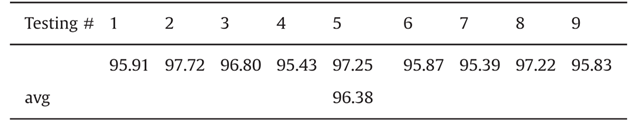
\includegraphics[width=1\linewidth]{images/17.png}
        \caption{Tasso di riconoscimento in percentule per le nove selezioni randomiche del training e test set}
        \label{fig:image4}
    \end{center}
\end{figure}

È stato dimostrato che il sistema ha una prestazione stabile utilizzando set di training e testing diversi. 
Il tasso di riconoscimento medio è significativamente più alto del metodo di confronto \cite{LearnExpresSpatTempManiFoldDynamFaceExpressReco}.

Un altro studio utilizzato per la predizione delle emozioni attraverso l’analisi delle Action Units è \cite{InferEmoFaceAUs}.
In questo studio viene proposto un metodo per mappare le AUs a sei emozioni:
\begin{itemize}
    \item anger,
    \item fear,
    \item happy,
    \item sad,
    \item surprise,
    \item disgust
\end{itemize}

Vengono selezionate delle Action Units, successivamente mappate alle emozioni attraverso relazioni statistiche e tecniche di matching.

Le relazioni fra le emozioni e le AUs sono collezionate come stringhe template che comprendono quelle più descrittive per ognuna delle emozioni trattate.

Le stringhe di template vengono poi computate usando un concetto chiamato discriminative power:

l’LCS, un metodo per approssimare il grado di coincidenza delle sottostringhe alla stringa di template, con l’applicazione del calcolo della prossimità fra le stringhe di test e la stringa di template della singola emozione.

Lo studio ha trovato che LCS è un metodo efficiente nella gestione di particolari problemi come il rilevamento errato delle AUs e aiuta a ridurre le predizioni false.

Il metodo proposto è stato testato su vari datasets:
\begin{itemize}
    \item CK+,
    \item ISL,
    \item FACS,
    \item JAFFE,
    \item Mind Reading,
    \item altri frame ripresi in condizioni in-the-wild
\end{itemize}

è stata poi effettuata una comparazione fra il metodo proposto e altri precedentemente presentati e si sono notati dei miglioramenti, sia sui datasets di benchmark che per quelli in-the-wild.\newpage

La procedura proposta basa il rilevamento delle AUs sul metodo offerto da \cite{RecoFaceExprMachLearnAppSpontBehav} e a seguire le Action Units vengono mappate con il metodo indicato nel paper, ed è visibile nell'immagine \ref{fig:image33}.
\begin{figure}
    \begin{center}    
        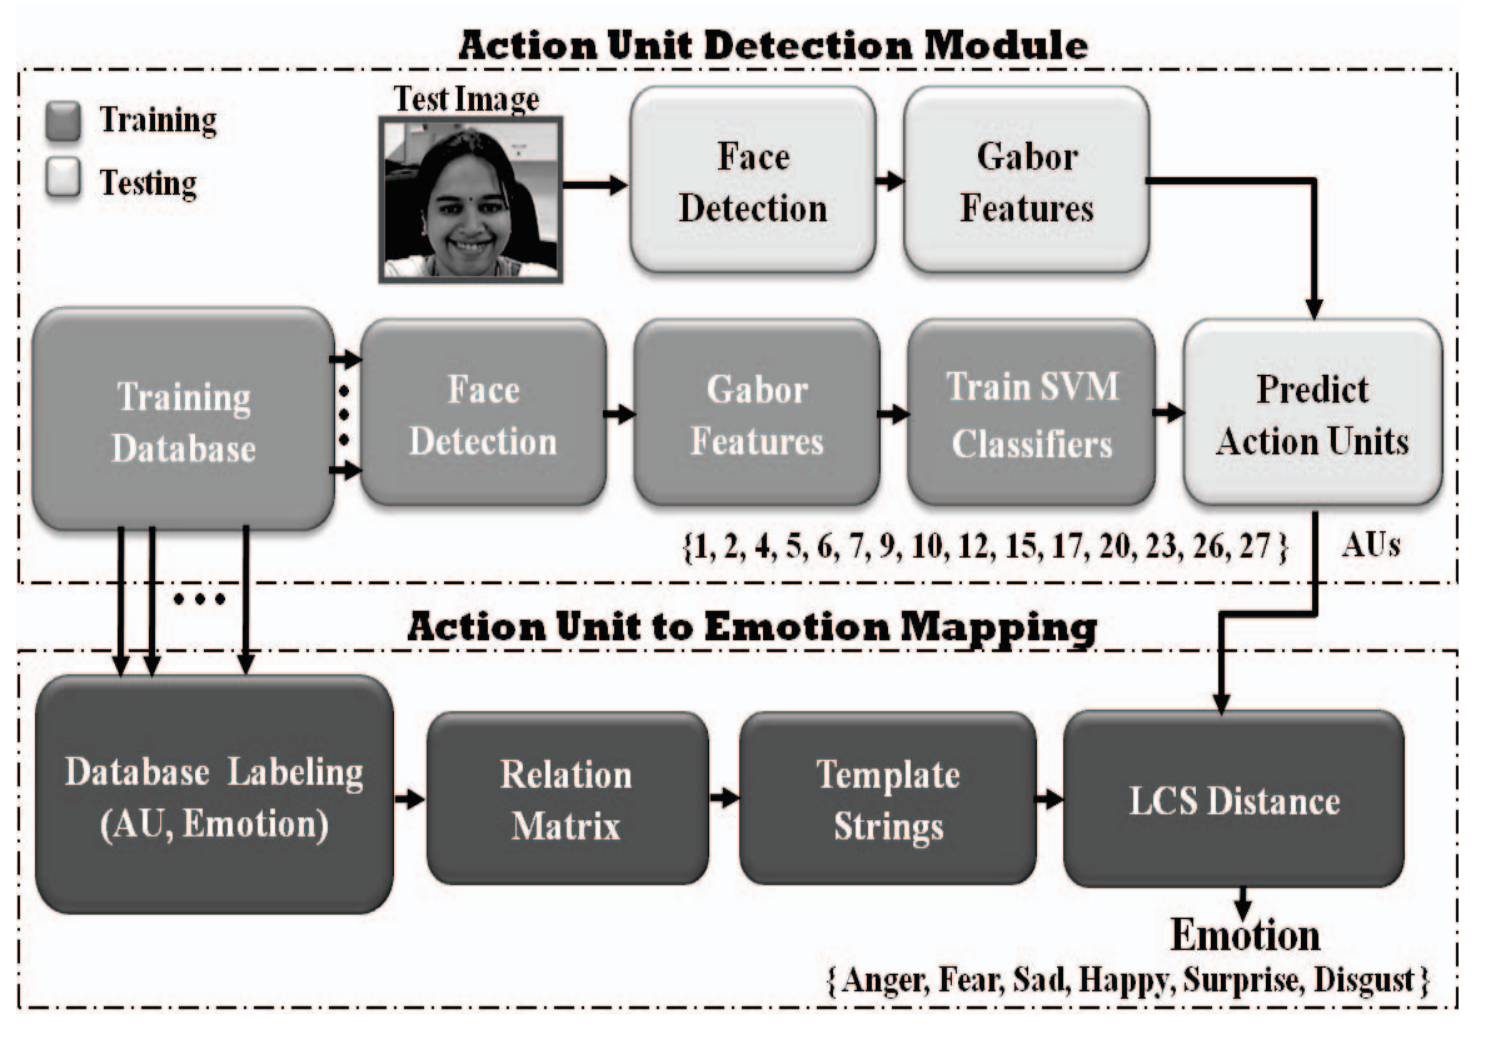
\includegraphics[width=0.7\linewidth]{images/18.png}
        \caption{Metodo di mappatura delle Action Units di \cite{RecoFaceExprMachLearnAppSpontBehav}}
        \label{fig:image33}
    \end{center}
\end{figure}

Per l’allenamento del modello volto al riconoscimento delle AUs sono state utilizzate 580 immagini dal CK+ dataset, e, per ognuna di queste, sono state effettuate varie modifiche alle immagini in modo da renderle adatte all’impiego; è stato applicato l’AdaBoost per la selezione delle feature al fine di ridurre la dimensione del vettore delle features, ed è stato utilizzato il Support Vector Machines (SVM) per il modello delle AUs.

Dopo un’attenta analisi del sistema FACS sono state scelte dai ricercatori quindici AUs, sufficienti per la rappresentazione delle sei emozioni che si sono proposti di identificare.

Le AUs rilevate vengono poi processate attraverso il modulo di mappatura per predire lo stato d’animo combaciante.

L’idea sulla quale il modello sviluppato in questo paper si fonda è che diversi metodi utilizzati per la rilevazione delle emozioni si basano su input (AUs) inaffidabili, in quanto sono presenti inevitabili errori nella localizzazione dei volti all’interno delle immagini.

È per questo che il loro metodo si concentra maggiormente sul trovare la correlazione fra le singole AUs e le emozioni che sulla diretta predizione di queste.

La relazione fra le Action Units e le sei emozioni si ottiene mediante un'analisi statistica del dataset di riferimento (CK+), etichettato sia per le emozioni che per le AUs. Le relazioni vengono acquisite sotto forma di una matrice relazionale derivata utilizzando un concetto chiamato discriminative power \cite{AutoInfereComplMentStatesVid}. 

Il discriminative power è definito come:
\[
H = P(Y_j|X_i) - P(Y_j|\overline{X_i})
\]
dove P(Yj |Xi) è la probabilità dell'azione $Yj$, dopo che $Xi$ è avvenuta, e $P(Yj | \overline{H_i})$ è la probabilità dell'azione $Yj$, dopo che l'emozione $H_i$ non è avvenuta. La dimensione di H rappresenta il potere discriminante di un'AU rispetto ad un'emozione.

La matrice relazionale viene ottenuta normalizzando H su tutte le AU per ciascuna delle emozioni. Pertanto, si ottengono pesi di associazione non lineari per ciascuna delle Action Unit, in base alla loro rilevanza per le emozioni calcolate servendosi dell'equazione sopra riportata.

La figura \ref{fig:image5} riporta la matrice di relazione calcolata per le sei emozioni. Qui, i valori positivi, rappresentati in bianco, indicano l'alta probabilità per un'AU di appartenere ad un'emozione; d’altra parte, i valori negativi, rappresentati in nero, indicano l'alta probabilità per un'AU di non essere associata ad un'emozione. 

Ad esempio, l'emozione happy è associata positivamente alle AU6, AU7, AU12, AU26 e negativamente alle AU1, AU2, AU5, AU9. 

I risultati sperimentali presentati dallo studio dimostrano che la matrice di relazione derivata è efficiente nell'identificazione delle azioni facciali altamente rilevanti e i loro pesi di associazione per le varie emozioni, e può quindi prevedere correttamente le emozioni.
\begin{figure}
    \begin{center}    
        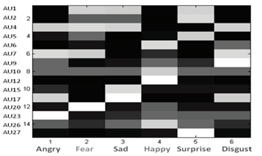
\includegraphics[width=0.6\linewidth]{images/19.png}
        \caption{Matrice di relazione calcolata sulle sei emozioni}
        \label{fig:image5}
    \end{center}
\end{figure}

Per ciascuna emozione sono state selezionate le prime N entrate da AU altamente discriminanti e queste sono state salvate come stringhe di template per i futuri abbinamenti delle Action Units. 

La lunghezza delle stringhe di template utilizzata è di cinque per gli esperimenti condotti dai ricercatori dello studio.\newpage
\begin{figure}
    \begin{center}    
        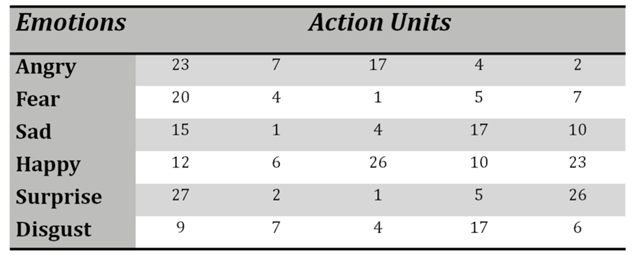
\includegraphics[width=1\linewidth]{images/20.png}
        \caption{Esempio di stringa template}
    \end{center}
\end{figure}

Date le stringhe con le Action Units per le immagini analizzate, queste vengono confrontate con le stringhe di template per trovare l'emozione corrispondente. 

Si utilizza la sotto sequenza comune più lunga (LCS) \cite{IntroToAlgo} per misurare la similarità tra le stringhe. LCS è un metodo per trovare la sotto sequenza più lunga fra tutte le sequenze date. 

In questo caso, una sotto sequenza è definita come una sequenza in cui le unità appaiono nello stesso ordine una rispetto all’altra, ma non necessariamente in modo contiguo. 

Ad esempio, nella stringa “ACTTGCG”, “ACT”, “ATTC” e “ACTTGC” sono tutte sotto sequenze. 

LCS permette "inserzioni", "eliminazioni" e "sostituzioni" delle singole AUs tra le stringhe. Questa caratteristica di LCS si è rivelata idonea per la predizione delle emozioni da stringhe di Action Units.

Per fare un esempio, data un'immagine di test, possono essere predette le combinazioni di AUs riportate nell’immagine \ref{fig:image6}.

In questo caso, la proprietà di eliminazione diventa importante per la mappatura delle diverse stringhe di Action Units come {AU12} o {AU6, AU12} o {AU6, AU12, AU26} all'emozione happy, poiché tutte indicano l’emozione di felicità pur mancando, alcune delle AU, nelle stringhe. 

Allo stesso modo, l'inserzione ha un ruolo nell’eliminazione delle AU rilevate erroneamente, come {AU1, AU4}, che comunque mappano l'emozione nella figura alla stringa di template che rappresenta l’emozione happy. 

Inoltre, permettere le sostituzioni aiuta a correggere gli errori di rilevazione che coinvolgono AU visivamente simili come AU12, AU20, AU23, e a predire l'emozione con un alto valore di confidenza. 

Viene evitata anche la mappatura errata di molte emozioni quando la stringa di test presenta errori considerevoli.
\begin{figure}
    \begin{center}    
        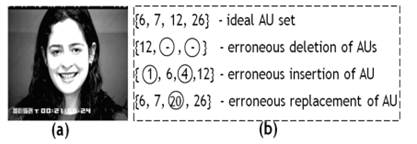
\includegraphics[width=1\linewidth]{images/21.png}
        \caption{Esempio di rilevamento delle Action Units}
        \label{fig:image6}
    \end{center}
\end{figure}

Ad esempio, in sostituzioni non condizionali, una stringa di test come 

\{{\colorbox{yellow}{AU4}, \colorbox{green}{AU6}, \colorbox{blue}{AU12}, \colorbox{cyan}{AU17}, \colorbox{magenta}{AU23}\}}, può essere mappata a 

\{{\colorbox{red}{AU1}, \colorbox{yellow}{AU4}, \colorbox{red}{AU10}, \colorbox{red}{AU15}, \colorbox{cyan}{AU17}\}} (tristezza) e 

\{{\colorbox{yellow}{AU4}, \colorbox{red}{AU6}, \colorbox{red}{AU7}, \colorbox{red}{AU9}, \colorbox{cyan}{AU17}\}} (disgusto) 

con un costo di sostituzione di "3". 

I risultati e l’accuratezza ottenuta dal metodo proposto dallo studio sui vari dataset utilizzati per valutarlo sono esposti nella tabella all'immagine \ref{fig:image7}:

\begin{figure}
    \begin{center}    
        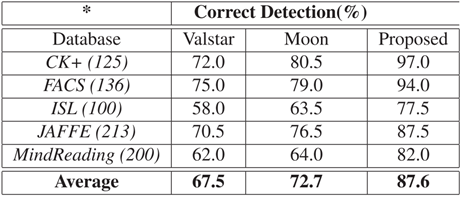
\includegraphics[width=1\linewidth]{images/22.png}
        \caption{Accuracy del metodo}
        \label{fig:image7}
    \end{center}
\end{figure}

\newpage

Analizzando altri papers sul soggetto, nessuno di questi mi è apparso particolarmente rilevante, in quanto carenti di metodologie che aggiungevano informazioni e metodi utili da unire ai lavori già ritrovati; inoltre i risultati di accuratezza e precisione ottenuti da questi sono inferiori rispetto agli studi già analizzati o insufficientemente migliori e necessitano di più risorse (tempo, quantità di dati e potere computazionale).

Ad esempio, in \cite{FaceEmoPredAUsDeepLearn} vengono confrontate le due principali tecniche di previsione delle emozioni facciali, ovvero le tecniche di apprendimento automatico (ML) e di deep learning (DL), in termini di accuratezza e livello di accountability. 
\begin{figure}
    \begin{center}    
        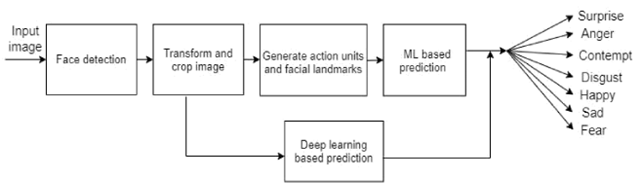
\includegraphics[width=1\linewidth]{images/23.png}
        \caption{Entrambi i process flow del riconoscimento delle emozioni facciali in \cite{FaceEmoPredAUsDeepLearn}}
    \end{center}
\end{figure}

Analizzando le due tecniche, i ricercatori hanno dimostrato che i modelli ML possono raggiungere risultati comparabili rispetto ai modelli DL. 

Nonostante la maggior parte delle ricerche recenti si siano focalizzate sulla costruzione di tecniche di Deep Learning per la predizione delle emozioni, si è scoperto che i modelli DL raggiungono prestazioni migliori a fronte di un costo elevato in termini di potenza di calcolo, di set di dati più grandi e di tempi di elaborazione più lunghi. 

Negli esperimenti sono stati conseguiti livelli di accuratezza del 86,66\% e dell'80\% rispettivamente per gli approcci DL e ML in termini di previsione delle emozioni; nonostante ciò, le tecniche di DL necessitano del supporto di una GPU ad alte prestazioni, mentre le tecniche ML possono ricoprire il proprio ruolo più velocemente anche senza il supporto di una GPU. 

Il beneficio più importante nell'utilizzo delle tecniche ML con le Action Units è la capacità di questi ultimi di poter giustificare l'emozione prevista in termini di contributo di ciascuna AU. 


\section{Studi che trattano campioni prelevati in scenari non controllati per una migliore precisione del modello}

Un altro problema trattato solo da \cite{PredLocStudEngagInTheWild} (fra i paper ritrovati a tema engagement e stati d’animo) e che invece ho notato più prominente all’interno della ricerca riguardo le emozioni FACS, è quello dei campioni denominati come “in-the-wild”.

Molti degli studi effettuati si concentrano su campioni prodotti in ambienti controllati, con nessun tipo di interferenza per quanto concerne i problemi che abitualmente si possono riscontrare quando invece si lavora con riprese che potrebbero avere una valenza anche quando le migliori condizioni non si presentano.

Come riporta \cite{AFEWVAdatabaseInTheWild}: “The videos are recorded under controlled conditions, e.g. illumination is uniform, background is static, and there is a limited amount of head pose variation and occlusion. Although a range of affective states are displayed and recorded, emotions are elicited by a limited number of tasks, e.g., in \cite{BelfastInducedNaturalEmotionDatabase}, all subjects underwent exactly the same tasks.”

Quindi i video creati in condizioni verificate, di luce uniforme, sfondo statico, con insufficienti variazioni nella posa delle persone, poca occlusione e dove le persone svolgono lo stesso compito non sono validi per creare un modello che possa effettuare delle predizioni veritiere da applicare ad ogni ambiente.

Per quanto riguarda la raccolta di immagini, negli studi “in the wild” è stato messo in atto il prelievo e la categorizzazione delle immagini da film, serie tv, e altri media che non rispettano gli standard imposti durante la creazione dei dataset prelevati invece in ambienti controllati \cite{AFEWVAdatabaseInTheWild}.

Per l’annotazione delle immagini sono stati consultati due annotatori esperti FACS AU che hanno individuato lo stato d’animo della/e persone presenti all’interno della scena presentata attraverso una piattaforma di tagging delle immagini.

Entrambi gli annotatori erano sempre presenti durante l’analisi dei singoli campioni ed hanno quindi potuto discutere ognuno dei casi incerti insieme; una volta concluse le prime analisi, sono stati inoltre ripresentati alcuni dei frame già analizzati agli stessi annotatori in modo da effettuare un’ulteriore verifica della loro consistenza, ed essi hanno dato la stessa annotazione l’87\% delle volte.

Per costruire il modello hanno poi utilizzato l’estrazione delle AU attraverso un sistema semi automatico, ed hanno utilizzato questi dati estratti per la costruzione del modello.

I risultati di queste analisi hanno portato alla conclusione che i modelli sviluppati attraverso raccolte di immagini prelevate in scenari controllati non portano necessariamente a risultati puntuali (o accurati) quando vengono applicati al mondo reale.
Una volta analizzati i sistemi utilizzati per l’elaborazione dei dati raccolti dai ricercatori che hanno redatto gli studi riportati precedentemente, ritengo ora necessario illustrare gli strumenti di cui si sono avvalsi.


\section{Cosa sono le AUs e il sistema FACS:}
FACS, acronimo di Facial Action Coding System, è un sistema di codifica delle espressioni facciali sviluppato dallo psicologo Paul Ekman e dal collega Wallace V. Friesen negli anni '70 \cite{PyFeat}.

Il sistema di codifica di FACS è composto da un insieme di codici numerici, o "Action Units" (AU), che rappresentano le azioni muscolari specifiche che avvengono durante le espressioni facciali. Ci sono 66 AUs, ciascuna delle quali rappresenta un'azione muscolare specifica, e ognuna di queste ha un codice numerico univoco.

La codifica delle FACS può essere utilizzata per identificare e descrivere le espressioni facciali in modo oggettivo e dettagliato. Ad esempio, un codificatore FACS identifica l'AU corrispondente al sollevamento di una delle due sopracciglia con codice 1, e l'AU corrispondente al sorriso con codice 12. 

Questi codici possono essere utilizzati per creare una descrizione dettagliata dell'espressione facciale di un individuo.

Le FACS sono state utilizzate in una vasta gamma di contesti, tra cui la ricerca scientifica, la valutazione clinica e la produzione di effetti speciali per il cinema e la televisione. 

Questo sistema è stato utilizzato con successo in molti contesti diversi ed è un metodo utile per descrivere le espressioni facciali in modo oggettivo e dettagliato. 

Sulla documentazione della libreria che ho utilizzato per l’estrazione delle AUs dal dataset aggregato ed utilizzato, è presente una tabella dove viene mostrato: il numero associato alla singola Action Unit, il loro relativo nome FACS, a quali muscoli della faccia sono correlate, la loro categoria FACS, le espressioni che vengono spesso legate a determinati valori di esse e i modelli che le utilizzano. Ho reso disponibile un estratto di questa \ref{Tab:Tabella_AUs} dove vengono presentate solo le Action Units utilizzate dalla libreria \cite{PyFeat} utilizzata per estrarre questi dati dalle immagini ma la tabella completa è consultabile sulla relativa pagina web.
\newpage
\begin{figure}
    \begin{center}    
        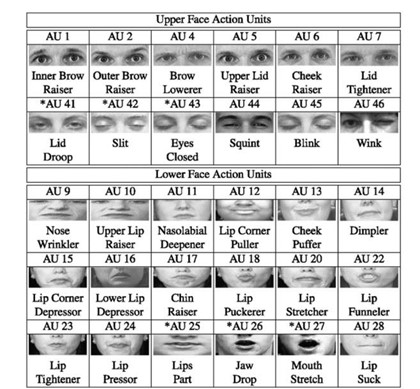
\includegraphics[width=1\linewidth]{images/10.jpg}
        \caption{Esempi di Action Units e le relativi sezioni facciali}
    \end{center}
\end{figure}


\section{Metodologie di tagging delle immagini del dataset}
Per quanto riguarda la classificazione delle immagini dei dataset, vari studi hanno fatto ricorso a tecniche diverse:
\begin{itemize}
    \item Self report sul proprio stato emotivo da parte delle persone da cui vengono prelevati i campioni per le analisi, attraverso questionari o in modo arbitrario
    \item Valutazione da parte di esperti, spesso più di uno, per assegnare uno stato emotivo alle singole immagini o video; o scelto in modo interamente arbitrario da parte del/dei valutatore/i o utilizzando come riferimento lo stato emotivo riportato dalla persona
    \item Classificazione attraverso metodi di clustering \cite{FacialExpresRecLocalBinaryPatt}
\end{itemize}

Strumenti utilizzati per effettuare la classificazione:
\begin{itemize}
    \item Piattaforma FEELTRACE (o altri software di annotazione manuale) che permette di registrare e analizzare i segnali EMG (Elettromiografici) e di misurare forza e durata delle risposte emotive dei partecipanti tramite una scala da 0 a 10 mentre i partecipanti osservano immagini, video o altre tipologie di stimoli emotivi \cite{AFEWVAdatabaseInTheWild}
    \begin{figure}[h]
        \centering    
            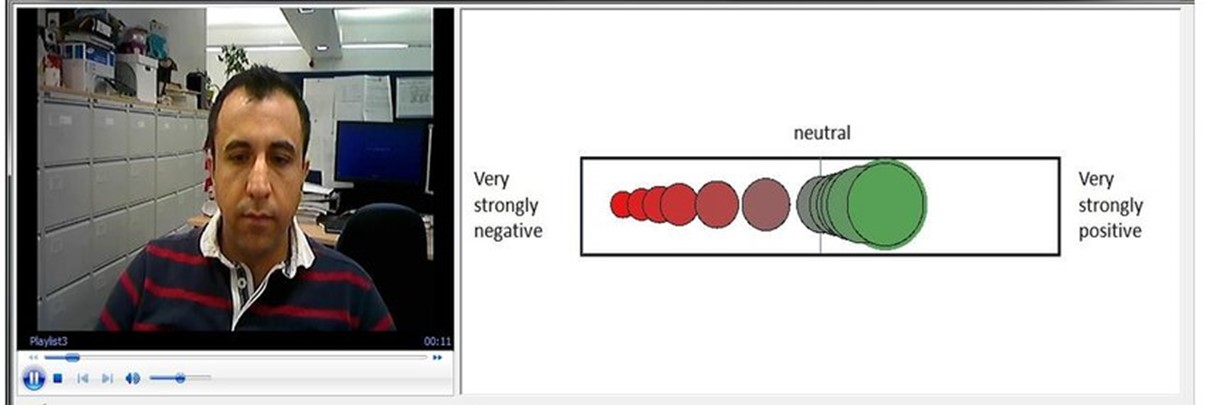
\includegraphics[width=0.5\linewidth]{images/11.jpg}
            \caption{Piattaforma FEELTRACE}
    \end{figure}
    \item Questionari a cui sottoporre i soggetti che vengono ripresi per la creazione del dataset
        \item \mbox{}\\[-\baselineskip]
        \begin{minipage}[t]{0.6\textwidth}
            In \cite{DAiSEE} è stata adoperata una tecnica di crowdsourcing: mediante la piattaforma Amazon Mechanical Turk (o MTurk) i ricercatori hanno specificato il task che si erano proposti di risolvere e hanno fornito i frame da analizzare. Questi sono stati poi suddivisi dalla piattaforma e categorizzati dai singoli individui (tale servizio è ovviamente retribuito)
        \end{minipage}\hfill
        \begin{minipage}[t]{0.3\textwidth}
            \centering
            \vspace{0pt}
            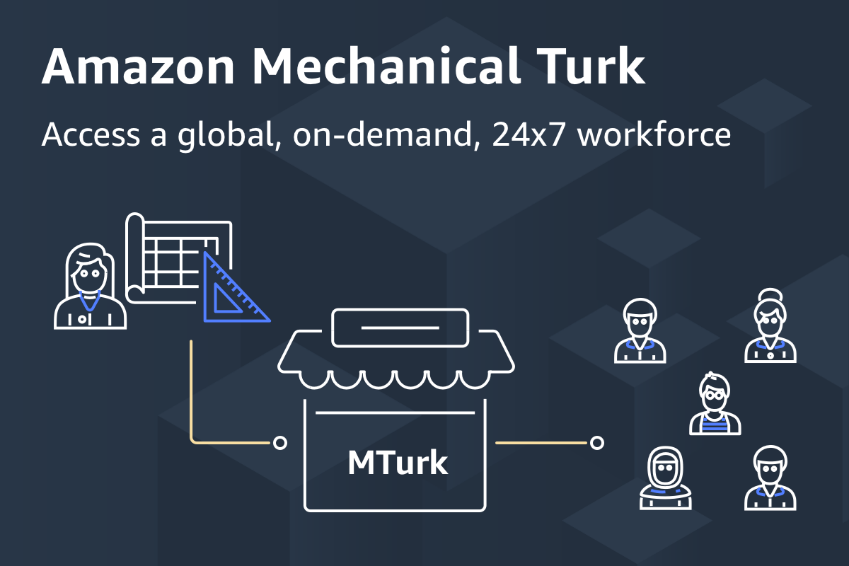
\includegraphics[width=\textwidth]{images/12.png}
        \end{minipage}
\end{itemize}


\section{Estrazione delle feature facciali dalle immagini e dai video dei dataset}
Per quanto concerne l’estrazione dei dati dalle immagini, i paper analizzati hanno adoperato diverse librerie e strumenti fra cui:
\begin{itemize}
    \item OpenCV: libreria open-source di computer vision di cui ci si può avvalere per il riconoscimento delle espressioni facciali. OpenCV contiene diverse funzioni per l'estrazione delle AUs, come la rilevazione delle linee facciali e la stima dei parametri di deformazione.
    \item dlib: libreria di machine learning open-source che somministra funzioni per la rilevazione e l'analisi dei volti nelle immagini. Dlib è in grado di rilevare le AUs attraverso l'utilizzo di una rete neurale convoluzionale (CNN) addestrata su un grande dataset di espressioni facciali.
    \item FaceReader: software commerciale sviluppato dalla società olandese Noldus Information Technology che ricorre ad algoritmi di analisi dell'emozione per registrare e classificare le AUs nelle immagini facciali. FaceReader è capace di riscontrare fino a 20 AUs e di classificarle in base alle emozioni ad essi associate.
    \item OpenFace: framework open-source di computer vision sviluppato dall'Università di Carnegie Mellon che offre funzioni per l'estrazione delle AUs e la rilevazione delle espressioni facciali. OpenFace sfrutta una combinazione di tecniche di machine learning e di analisi geometrica per rilevare le AUs.
    \item FACET: software commerciale sviluppato dalla società americana Emotient che impiega una combinazione di tecniche di computer vision e di analisi dell'emozione per rilevare e classificare le AUs nelle immagini facciali. FACET è in grado di rilevare fino a 20 AUs e di classificarle in base alle emozioni associate.
    \item DeepFaceLab: software open-source che utilizza le deep neural networks per l'analisi dell'immagine e la manipolazione dei lineamenti. Può essere strumentalizzato per l'estrazione delle AUs da immagini facciali. 
\end{itemize}

Per il progetto di tesi ho invece deciso di utilizzare:

Pyfeat: libreria open-source sviluppata in Python per l'estrazione delle feature facciali dalle immagini. Pyfeat si basa sulla fruizione di un insieme di funzioni matematiche, dette funzioni di base, per descrivere la forma e l'aspetto delle suddette espressioni. 
    
Tali funzioni di base sono rappresentate da immagini di capacità espressiva standardizzate, quali sorriso o rabbia, create e validate da esperti di psicologia e neuroscienze. 

La libreria Pyfeat fa uso di queste funzioni di base per il calcolo di un insieme di feature facciali, fra cui la forma del viso, la posizione degli occhi, la sagoma delle sopracciglia, la posizione della bocca e le Action Units. 

Pyfeat è in grado di estrarre un insieme completo di 280 feature facciali, le 2D FACS (Facial Action Coding System), anch’esse validate da esperti di psicologia e neuroscienze. 

Pyfeat può essere impiegato per diverse applicazioni di analisi facciale, come la rilevazione delle emozioni, l'analisi del comportamento non verbale e la diagnostica medica. 

Ho ritenuto opportuno ricorrere a questa libreria per l’estrazione delle AUs in quanto affidabile e agevole nell’utilizzo, soprattutto attraverso le funzioni CUDA della libreria che mi hanno permesso di velocizzare di molto il processing delle immagini contenute nei dataset ritrovati; inoltre, nessuno degli studi analizzati ha adoperato questa libreria.
\begin{figure}
    \begin{center}    
        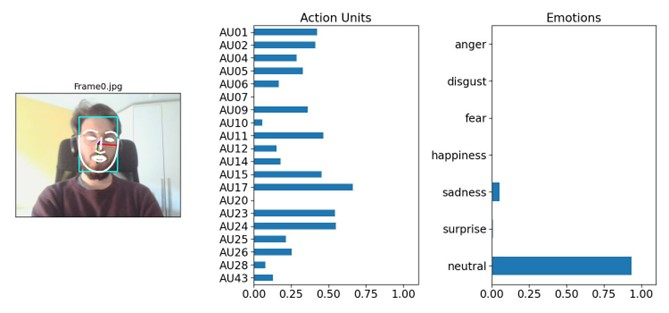
\includegraphics[width=1\linewidth]{images/13.jpg}
        \caption{Esempio di estrazione AUs tramite py-feat}
    \end{center}
\end{figure}

Dopo aver analizzato i sistemi impiegati per l’elaborazione delle informazioni ottenute dalle immagini ed aver illustrato il processo di estrapolazione di questi dati, reputo possibile la creazione di un dataset ricavato dall’unione di alcuni dei datasets citati precedentemente per lo studio di questa tesi.

\newpage

\section{Unione dei dataset ritrovati e relativa categorizzazione delle immagini all’interno di questo}

I dataset utili ritrovati sono il DAiSEE \cite{DAiSEE} e il Student-engagement-dataset \cite{StudEngagDataset}.

\begin{itemize}
    \item DAiSEE presenta i seguenti mood:
    \begin{itemize}
        \item Boredom
        \item Engagement
        \item Confusion
        \item Frustration
    \end{itemize}
    \item Tutte con valore compreso fra 0 e 3:
    \begin{itemize}
        \item Inizialmente è stato chiesto ai labelers di annotare i frame a loro presentati con uno di questi tre tag:
        \begin{itemize}
            \item Looking at their paper
            \item Looking at their screen
            \item Wandering
        \end{itemize}
            
        Ognuno dei frame è stato assegnato almeno a tre persone, la label “vincente”, o meglio più frequente, è stata poi attribuita ai singoli frame.

        Infine, in base ai risultati ottenuti attraverso questa categorizzazione, conseguita via crowdsourcing, è stato conferito un valore fra 0 (non corrispondente) e 3 (del tutto corrispondente) ad ognuna delle classi precedentemente elencate.
    \end{itemize}
    \item Student engagement dataset, invece, presenta i seguenti mood:
    \begin{itemize}
        \item Confused (macro categoria: engaged)
        \item Engaged (macro categoria: engaged)
        \item Frustrated (macro categoria: engaged)
        \item Bored (macro categoria: not engaged)
        \item Drowsy (macro categoria: not engaged)
        \item Looking away (macro categoria: not engaged)
    \end{itemize}
\end{itemize}

Per la realizzazione del mio dataset ho ritenuto giusto attenermi alle classi proposte dallo Student Engagement dataset, in quanto propone più labels di cui usufruire.

Per mettere in atto ciò, è stato necessario unire i samples all’interno di DAiSEE ai samples dello student engagement dataset, per mezzo delle classi corrispondenti.

DAiSEE è provvisto di un maggior numero di samples, in quanto non solo racchiude molti più file, ma questi stessi sono video e non immagini, come nello student engagement dataset, naturalmente suddivisi in frame (2 immagini per ogni secondo di video).

Le classi che non trovano corrispondenza fra i due dataset (Drowsy e Looking away) potrebbero risultare meno frequenti e accurate nel riconoscimento; ho comunque preferito conservarle in quanto permettono una classificazione più ampia.

DAiSEE è un dataset realizzato tenendo in considerazione la questione “in-the-wild” e risulta quindi perfetto per lo studio proposto da questa tesi.

Lo student engagement dataset non è stato creato da una fonte autorevole e certificata come il DAiSEE ma, sfogliando le immagini presenti in esso, è possibile notare come gli scenari ripresi in questo dataset (ambienti di studio casalinghi) le immagini al suo interno risultino simili a quelle presentate nel DAiSEE e quindi della tipologia interessata.

\begin{table}[htb]
\small
\caption{estratto tabella AUs}
\label{Tab:Tabella_AUs}
\centering
    \begin{adjustbox}{angle=90}
        \begin{tabular}{|c|l|l|l|}
            \hline
            AU1 & Inner Brow Raiser & Frontalis (medial) & sadness, surprise, fear \\
            \hline
            AU2 & Outer Brow Raiser & Frontalis (lateral) & surprise, fear \\
            \hline
            AU4 & Brow Lowerer & Procerus, Depressor Supercilii, Corrugator Supercilii & sadness, fear, anger \\
            \hline
            AU5 & Upper Lid Raiser & Levator Palpebrae Superioris, Superior Tarsal Muscle & surprise, fear, anger \\
            \hline
            AU6 & Cheek Raiser & Orbicularis Oculi (orbital) & happiness, disgust, contempt \\
            \hline
            AU7 & Lid Tightener & Orbicularis Oculi (palpebral) & fear, anger \\
            \hline
            AU9 & Nose Wrinkler & Levator Labii Superioris Alaeque Nasi & disgust \\
            \hline
            AU10 & Upper Lip Raiser & Levator Labii Superioris & \\
            \hline
            AU11 & Nasolabial Deepener & Zygomaticus Minor & disgust, fear \\
            \hline
            AU12 & Lip Corner Puller & Zygomaticus Major & happiness, contempt \\
            \hline
            AU14 & Dimpler & Buccinator & contempt \\
            \hline
            AU15 & Lip Corner Depressor & Depressor Anguli Oris & sadness, disgust \\
            \hline
            AU17 & Chin Raiser & Mentalis & disgust \\
            \hline
            AU20 & Lip Stretcher & Risorius, Platysma & fear \\
            \hline
            AU23 & Lip Tightener & Orbicularis Oris & anger \\
            \hline
            AU24 & Lip Pressor & Orbicularis Oris & \\
            \hline
            AU25 & Lip Part & Depressor Labii Inferioris & happiness, surprise, fear \\
            \hline
            AU26 & Jaw Drop & Masseter, Temporalis, Medial Pterygoid & fear, surprise \\
            \hline
            AU28 & Lip Suck & Orbicularis Oris & \\
            \hline
            AU43 & Eyes Closed & Levator Palebrae Superioris (relaxation) & behavioral \\
            \hline
        \end{tabular}
    \end{adjustbox}
\end{table}

\chapter{Tecnologie, strumenti e librerie utilizzate}
Questo capitolo tratterà le tecnologie, gli strumenti, le librerie e gli algoritmi utilizzati per la realizzazione dei modelli predittivi e dell’interfaccia successivamente creata. 
\section{Tecnologie}
\subsection{Machine Learning}

Il Machine Learning, o apprendimento automatico, è un campo di studio che si occupa di sviluppare algoritmi in grado di perfezionarsi automaticamente mediante l'esperienza acquisita tramite l'utilizzo dei dati. 

Gli algoritmi di Machine Learning creano modelli matematici a partire da dati di esempio chiamati "dati di training", in modo da poter attuare predizioni o prendere decisioni senza essere esplicitamente programmati per farlo. 

Esistono tre categorie di approcci di Machine Learning: l'apprendimento supervisionato, l'apprendimento non supervisionato e l'apprendimento per rinforzo.
\begin{itemize}
    \item L'apprendimento supervisionato consiste nell’indicare al calcolatore una regola generale che mappi gli input e gli output desiderati. 
    
    L'algoritmo di apprendimento è provvisto di dati di input di esempio e degli output corrispondenti e, attraverso successive iterazioni, viene successivamente costruito un modello matematico che può essere sfruttato per predire l'output associato ad un nuovo input.
    
    \item L'apprendimento non supervisionato invece, non fornisce all'algoritmo di apprendimento le etichette desiderate. 
    
    In questo caso, l'algoritmo di apprendimento deve necessariamente estrapolare le informazioni significative dai dati di input pur non essendo a conoscenza dell'output desiderato.
    
    \item L'apprendimento per rinforzo prevede che un programma interagisca con un ambiente dinamico con lo scopo di raggiungere un obiettivo specifico, ad esempio guidare un veicolo o vincere un gioco contro un avversario. 
\end{itemize}
Durante le varie iterazioni il programma riceve un feedback sotto forma di premio e cerca di massimizzare il suo “punteggio”, in modo da imparare e raggiungere l'obiettivo prefissato.

\subsection{Computer Vision}
La Computer Vision è un campo interdisciplinare che si occupa della capacità dei computer di acquisire conoscenza da immagini o video, cercando di replicare il complesso meccanismo alla base dell'apparato visivo umano. 

Questa utilizza metodi per l'acquisizione e l'analisi di immagini digitali in modo da estrarre dati multidimensionali dal mondo reale e produrre informazioni numeriche o simboliche. 

Si avvale pertanto anche di conoscenze di geometria, fisica, statistica e della teoria dell'apprendimento per descrivere il mondo in modo sensato, producendo risultati che possono indirizzarci alla corretta linea d'azione.

\subsection{Cuda} 
CUDA® \cite{CUDA} è una piattaforma di calcolo parallelo, un modello di programmazione sviluppato da NVIDIA per il calcolo generale su unità di elaborazione grafica (GPU). 

Per mezzo di CUDA, gli sviluppatori possono ampliare significativamente la velocità delle applicazioni di calcolo sfruttando la potenza delle GPU.

Nelle applicazioni dotate di accelerazione GPU, la parte sequenziale del carico di lavoro viene eseguita sulla CPU, ottimizzata per le prestazioni single-threaded, mentre la parte computazionalmente intensiva dell’applicazione viene realizzata su migliaia di core GPU in parallelo. 

Quando ci si avvale di CUDA, gli sviluppatori hanno la possibilità di programmare in linguaggi popolari come C, C++, Fortran, Python e MATLAB, esprimendo il parallelismo attraverso estensioni sotto forma di poche parole chiave di base.
Il toolkit CUDA di NVIDIA fornisce tutto il necessario per sviluppare applicazioni con accelerazione GPU.

Il toolkit CUDA include librerie accelerate su GPU, un compilatore, strumenti di sviluppo e il runtime CUDA.

\begin{figure}
    \begin{center}    
        
\includegraphics[width=0.9\linewidth]{images/image1.png}
        \caption{CUDA}
    \end{center}
\end{figure}

\section{Strumenti}
\subsection{Visual Studio Code}
Visual Studio Code è un editor di testo sviluppato da Microsoft per Windows, Linux e macOS, che supporta il debugging, il controllo Git integrato, la Syntax Highlighting, l'IntelliSense, lo Snippet e il refactoring del codice. 

Visual Studio Code supporta molteplici linguaggi e funzionalità aggiuntive grazie alla possibilità di installare dei plugin disponibili attraverso un repository centrale che presenta, oltre a diverse estensioni fornite direttamente da Microsoft, innumerevoli estensioni rese disponibili dalla community. 

\begin{figure}[h]
    \begin{center}
        \begin{minipage}[b]{0.35\linewidth}
            \centering
            
\includegraphics[width=\linewidth]{images/image2.png}
        \end{minipage}
        \begin{minipage}[b]{0.35\linewidth}
            \centering
            
\includegraphics[width=\linewidth]{images/image3.png}
        \end{minipage}
    \end{center}
    \caption{Visual studio code e python}
\end{figure}

\section{Librerie}
\subsection{Pandas}
La libreria software open source Pandas è stata sviluppata per il linguaggio di programmazione Python, ed è utilizzata per la manipolazione e l'analisi dei dati. Con Pandas è possibile effettuare operazioni su tabelle numeriche e serie temporali mediante le sue strutture dati. 

Il termine"Pandas" deriva dal termine econometrico "Panel Data", appellativo attribuito a un insieme di dati contenenti osservazioni sugli stessi individui durante più periodi di tempo.

\begin{figure}
    \begin{center}    
        
\includegraphics[width=0.9\linewidth]{images/image4.jpeg}
        \caption{Pandas}
    \end{center}
\end{figure}

\subsection{Tqdm}
La libreria Python tqdm \cite{Tqdm} è uno strumento molto utile per la visualizzazione di barre di avanzamento durante i cicli di elaborazione nel codice. 

Il nome "tqdm" deriva dall'unione della parola araba "taqaddum" che significa "progresso" ed è l'abbreviazione di "te quiero demasiado" (ti amo troppo) in spagnolo. 

Per servirsi della libreria basta inserire qualsiasi iterabile (liste, dizionari, tuple e set) nel metodo della libreria, in questo modo \mintinline[bgcolor=bg]{python}{tqdm(iterable)}. 

La libreria funziona su qualsiasi piattaforma ed è completamente indipendente dalle dipendenze. 

Durante l'estrazione delle Action Units la libreria tqdm ha fornito una stima precisa del tempo necessario per completare l'elaborazione, consentendo di monitorare l'avanzamento del processo in tempo reale. 

Nonostante l'utilizzo della tecnologia CUDA per accelerare le analisi, la grande quantità di immagini da elaborare ha richiesto molto tempo. 

La presenza di tqdm è stata quindi di fondamentale importanza, in quanto ha permesso di gestire efficacemente l'elaborazione dei dati, evitando eventuali problemi tecnici, garantendo risultati accurati ed affidabili e portandomi a riconsiderare delle scelte algoritmiche, non efficientissime, inizialmente intraprese. 

In sintesi, la libreria Python tqdm è uno strumento prezioso per semplificare l'elaborazione di grandi quantità di dati, fornendo una stima del tempo rimanente e consentendo di pianificare il lavoro in modo efficiente.

\begin{figure}
    \begin{center}    
        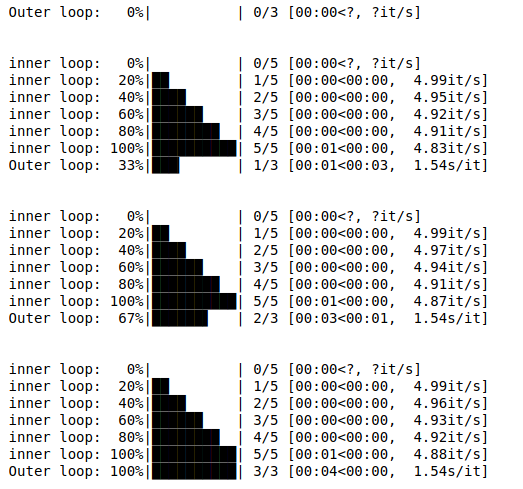
\includegraphics[width=0.9\linewidth]{images/image5.png}
        \caption{Esempio di utilizzo di tqdm}
    \end{center}
\end{figure}

\subsection{Pickle}
La libreria pickle è molto versatile e può essere utilizzata per salvare e ripristinare qualsiasi tipo di oggetto Python, inclusi dizionari, liste, tuple, classi e istanze di oggetti personalizzati. 

Inoltre, pickle supporta anche la serializzazione di oggetti multipli in un unico file, rendendo più semplice l'organizzazione dei dati. 

La libreria offre anche diverse opzioni per controllare il comportamento della serializzazione, come la scelta del protocollo di serializzazione e la possibilità di escludere alcuni attributi dall'oggetto da serializzare.

Una caratteristica importante della libreria pickle è che gli oggetti serializzati possono essere utilizzati su diverse piattaforme e versioni di Python, purché il protocollo di serializzazione utilizzato sia compatibile. 

Ciò significa che un oggetto serializzato su un computer Windows con Python 3.9 potrebbe essere deserializzato su un computer Linux con Python 2.7, ad esempio. 

Tuttavia, è importante notare che non tutti gli oggetti possono essere serializzati correttamente, come ad esempio le funzioni e le istanze di oggetti di alcune librerie Python. 

Inoltre, la compatibilità tra diverse versioni di Python non è garantita in tutti i casi; quindi, è necessario prestare attenzione a eventuali incompatibilità.

\begin{figure}
    \begin{center}    
        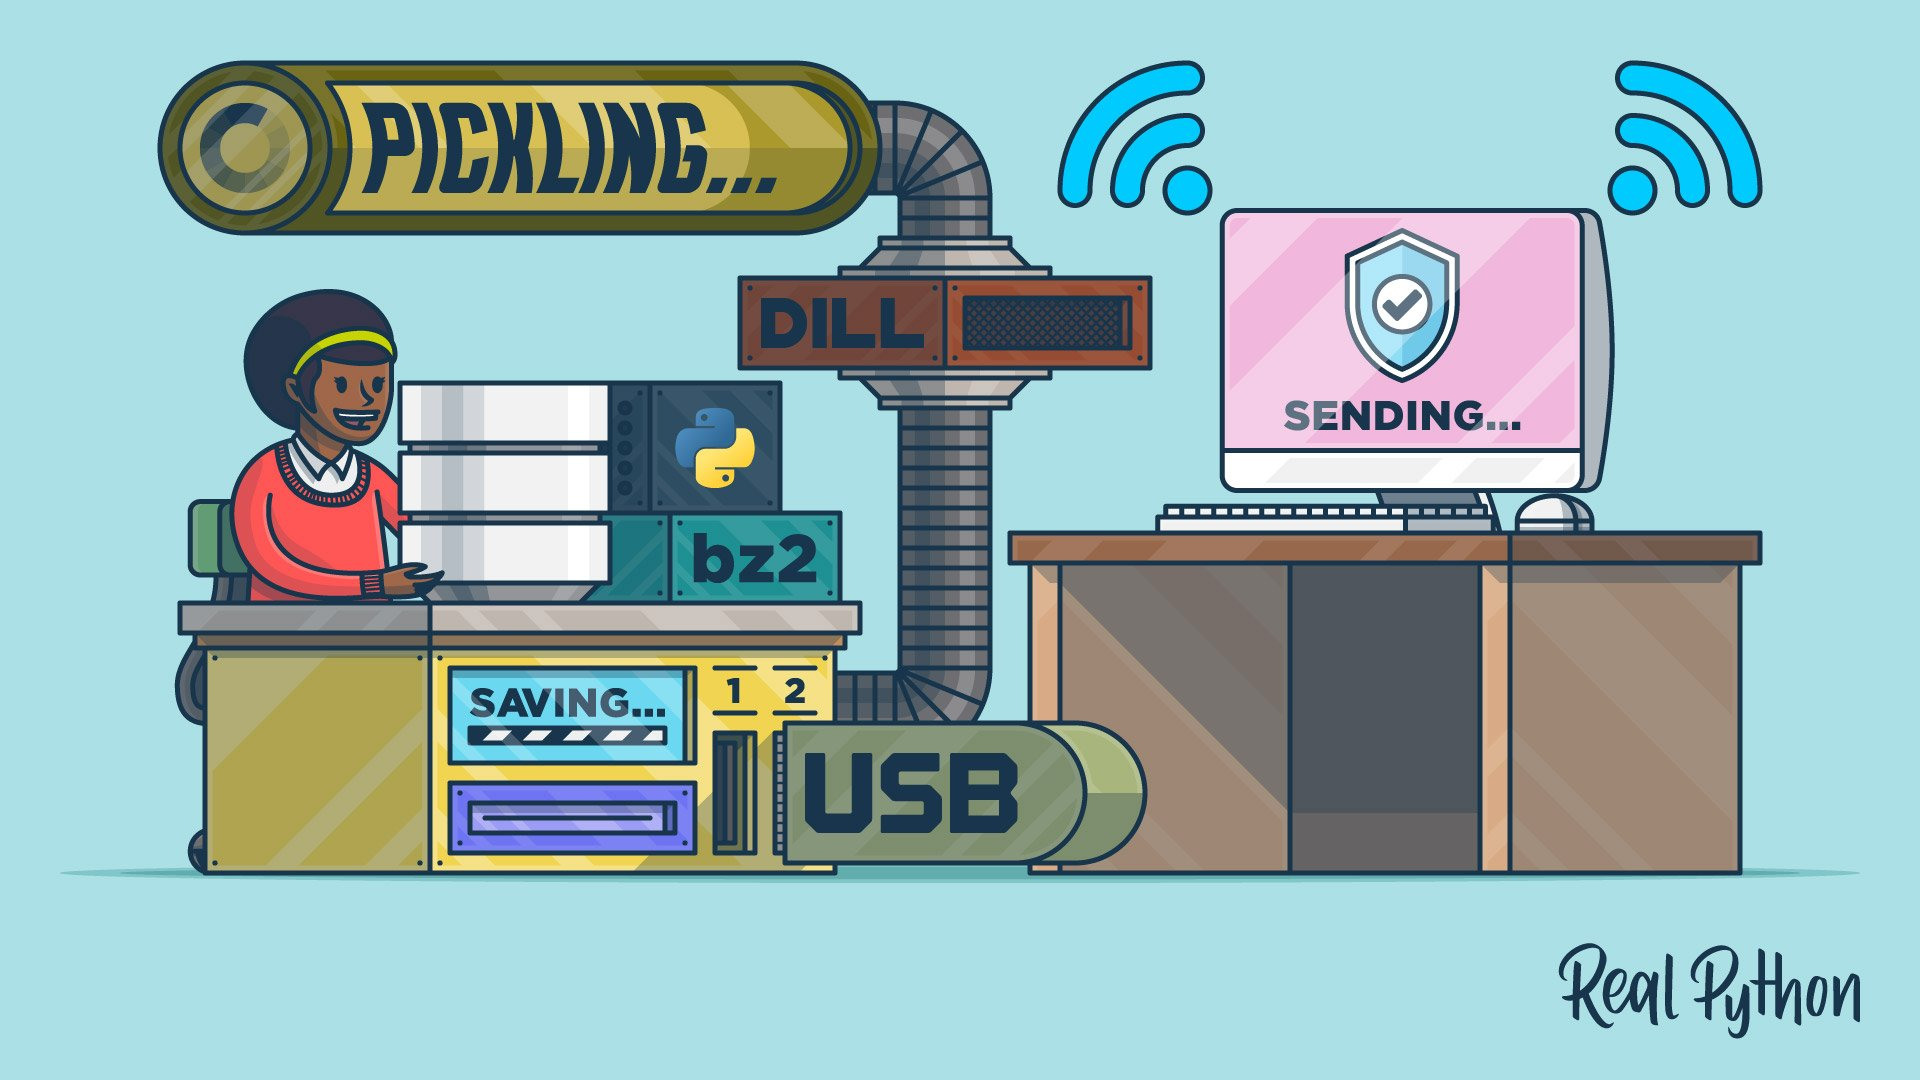
\includegraphics[width=1\linewidth]{images/image6.jpeg}
        \caption{Pickle}
    \end{center}
\end{figure}

\subsection{Torch}
PyTorch è un popolare framework open-source di deep learning che consente agli sviluppatori di creare modelli di intelligenza artificiale in modo rapido ed efficiente. È stato sviluppato originariamente da Facebook AI Research, guadagnandosi una grande popolarità per la sua facilità d'utilizzo, la sua flessibilità e la sua scalabilità.

Una delle sue principali caratteristiche è la sua architettura a flusso di dati (data flow), la quale rende il framework particolarmente adatto per le applicazioni di deep learning. 

Inoltre, PyTorch è dotato di un'ampia gamma di librerie e strumenti come PyTorch Lightning, che mirano a semplificare lo sviluppo di modelli di intelligenza artificiale.

Questa libreria è anche conosciuta per la sua flessibilità e scalabilità, in quanto permette di creare modelli di deep learning sia per computer singoli che per cluster di computer. 

In aggiunta, supporta una vasta gamma di piattaforme hardware, come CPU, GPU e TPU, il che la rende adatta per le applicazioni in ambiti come il machine learning, la visione artificiale e il linguaggio naturale.

\begin{figure}
    \begin{center}    
        
\includegraphics[width=0.9\linewidth]{images/image7.png}
        \caption{PyTorch}
    \end{center}
\end{figure}

\subsection{OpenCV}
OpenCV (Open Source Computer Vision Library) \cite{OpenCv} è una libreria software open source finalizzata all’ambito della computer vision e del machine learning. 

È stata ideata per fornire un'infrastruttura comune per le applicazioni di computer vision e per accelerare l'uso della percezione automatica nei prodotti commerciali. 

In quanto prodotto con licenza Apache 2, OpenCV facilita l'utilizzo e la modifica del codice da parte delle aziende.

La libreria contiene più di 2500 algoritmi ottimizzati, che includono un insieme completo di algoritmi di computer vision e machine learning sia classici che all'avanguardia. 

Questi algoritmi possono essere utilizzati per:
\begin{itemize}
  \item rilevare e riconoscere volti, 
  \item identificare oggetti, 
  \item classificare azioni umane nei video, 
  \item tracciare il movimento della telecamera, 
  \item tracciare oggetti in movimento, 
  \item estrarre modelli 3D di oggetti, 
  \item produrre cluster di punti 3D da telecamere stereo, 
  \item unire immagini per produrre un'immagine ad alta risoluzione di un'intera scena, 
  \item trovare immagini simili da un database di immagini, 
  \item rimuovere gli occhi rossi dalle immagini scattate con il flash, 
  \item seguire i movimenti degli occhi, 
  \item riconoscere paesaggi,
  \item creare marker per sovrapporli alla realtà aumentata, ecc. 
\end{itemize}

OpenCV ha più di 47mila utenti nella sua comunità e un numero stimato di download superiore a 18 milioni.

Oltre alle aziende ben consolidate come Google, Yahoo, Microsoft, Intel, IBM, Sony, Honda e Toyota, esistono molte startup come Applied Minds, VideoSurf e Zeitera che ne fanno un uso intensivo. 

Esso è impiegato per molteplici applicazioni, tra cui unire immagini di Street View, rilevare intrusioni in video di sorveglianza in Israele, monitorare l'equipaggiamento minerario in Cina, aiutare i robot a navigare e raccogliere oggetti presso Willow Garage, rilevare gli incidenti di annegamento in piscina in Europa, eseguire arte interattiva in Spagna e New York, controllare le piste di atterraggio per rilevare detriti in Turchia, ispezionare le etichette sui prodotti nelle fabbriche di tutto il mondo e per la rapida rilevazione dei volti in Giappone.

È provvisto di interfacce per C++, Python, Java e MATLAB e supporta Windows, Linux, Android e Mac OS. 

Ci sono oltre 500 algoritmi e circa 10 volte tante funzioni che compongono o supportano questi ultimi.

OpenCV è scritto nativamente in C++ e ha un'interfaccia template che funziona perfettamente con i contenitori STL.

\begin{figure}
    \begin{center}    
        
\includegraphics[width=0.5\linewidth]{images/image8.png}
        \caption{OpenCV}
    \end{center}
\end{figure}

\subsection{Scikit-learn}
Scikit-learn \cite{scikitLearn} (precedentemente conosciuto come scikits.learn e anche noto come sklearn) è una libreria di machine learning gratuita per il linguaggio di programmazione Python. 

Essa include vari algoritmi di classificazione, regressione e clustering, tra cui support-vector machine, random forest, gradient boosting, k-means e DBSCAN, ed è progettata per funzionare in combinazione con le librerie numeriche e scientifiche di Python, come NumPy e SciPy. 

Il progetto scikit-learn è nato come progetto Google Summer of Code dal data scientist francese David Cournapeau, originariamente chiamato scikits.learn. Il nome del progetto deriva dal concetto di "SciKit" (SciPy Toolkit), un'estensione di terze parti separata e distribuita per SciPy. 

Il codice originale è stato successivamente riscritto da altri sviluppatori. Nel 2010, i contribuenti Fabian Pedregosa, Gaël Varoquaux, Alexandre Gramfort e Vincent Michel dall'Istituto francese per la ricerca in informatica e automazione a Saclay, hanno preso il comando del progetto rilasciando in  seguito la prima versione pubblica della libreria il 1 febbraio 2010. Nel novembre 2012, scikit-learn e scikit-image sono stati descritti come due delle "scikits library" meglio conservate e popolari. 
Nel 2019 si è poi stimato che scikit-learn fosse una delle librerie di machine learning più popolari su GitHub.

Scikit-learn è principalmente scritto in Python e utilizza ampiamente NumPy per l'algebra lineare ad alta prestazione e le operazioni sugli array. 

Inoltre, alcuni algoritmi core sono scritti in Cython per migliorare le prestazioni. Support vector machine è implementato da un wrapper Cython intorno a LIBSVM; la regressione logistica e le macchine a vettori di supporto lineari da un wrapper simile intorno a LIBLINEAR. In tali casi, estendere questi metodi con Python potrebbe non essere possibile.

Scikit-learn si integra bene con molte altre librerie di Python come Matplotlib e Plotly per la visualizzazione dei dati, NumPy per la vettorizzazione degli array, Pandas dataframes, SciPy e molte altre.

\begin{figure}
    \begin{center}    
        
\includegraphics[width=0.7 \linewidth]{images/image9.png}
        \caption{SciKit learn}
    \end{center}
\end{figure}

\subsection{Py-Feat}
Per il progetto di tesi ho invece deciso di utilizzare:

Py-Feat: libreria open-source sviluppata in Python per l'estrazione delle feature facciali dalle immagini. Pyfeat si basa sulla fruizione di un insieme di funzioni matematiche, dette funzioni di base, per descrivere la forma e l'aspetto delle suddette espressioni. 
    
Tali funzioni di base sono rappresentate da immagini di capacità espressiva standardizzate, quali sorriso o rabbia, create e validate da esperti di psicologia e neuroscienze. 

La libreria Pyfeat fa uso di queste funzioni di base per il calcolo di un insieme di feature facciali, fra cui la forma del viso, la posizione degli occhi, la sagoma delle sopracciglia, la posizione della bocca e le Action Units. 

Pyfeat è in grado di estrarre un insieme completo di 280 feature facciali, le 2D FACS (Facial Action Coding System), anch’esse validate da esperti di psicologia e neuroscienze. 

Pyfeat può essere impiegato per diverse applicazioni di analisi facciale, come la rilevazione delle emozioni, l'analisi del comportamento non verbale e la diagnostica medica. 

Ho ritenuto opportuno ricorrere a questa libreria per l’estrazione delle AUs in quanto affidabile e agevole nell’utilizzo, soprattutto attraverso le funzioni CUDA della libreria che mi hanno permesso di velocizzare di molto il processing delle immagini contenute nei dataset ritrovati; inoltre, nessuno degli studi analizzati ha adoperato questa libreria.
\begin{figure}
    \begin{center}    
        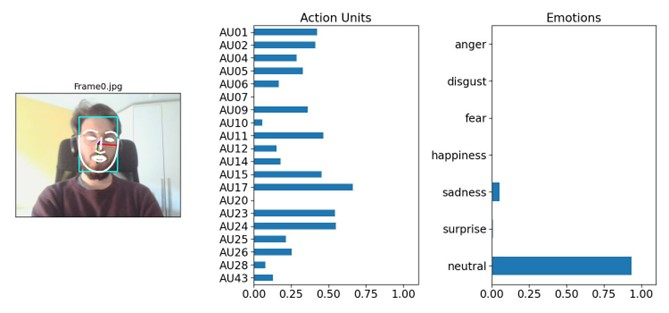
\includegraphics[width=1\linewidth]{images/13.jpg}
        \caption{Esempio di estrazione AUs tramite py-feat}
    \end{center}
\end{figure}
\chapter{Dataset risulato}
Come anticipato nel primo capitolo, il dataset di immagini utilizzato per il mio caso di studio è il risultato dell’unione dei due dataset Student engagement dataset\cite{StudEngagDataset} e DAiSEE\cite{DAiSEE}.

In principio le immagini e i video al loro interno sono state elaborate attraverso la libreria py-feat per ottenere le misure delle Action Units.

Le labels risultanti e il numero di sample per ognuna di queste sono:
\begin{itemize}
\item engaged con 55707 samples
\item bored con 16086 samples
\item confused con 1041 samples
\item looking away con 409 samples
\item frustrated con 893 samples
\item drowsy con 240 samples
\end{itemize}

con un totale di 74322 immagini (o frame estratti da video) per le quali sono stati generati i dati relativi alle Action Units.

\section{Generazione descrizione in linguaggio naturale}
Ho aggiunto una descrizione in linguaggio naturale di ogni immagine utilizzando il seguente codice:

\begin{minted}[bgcolor=bg]{python}
if value and value >= 0.5:
    return outAU.get ("FACS Name") + ", using the muscles: " + 
        outAU.get ("Muscles") + ", with a value of " + str (value) + "; "
else:
    return ""
\end{minted}
Questo algoritmo verifica inizialmente che il valore dell’Action Unit passato in input al metodo (non riportato interamente in quanto prevede azioni preliminari trascurabili) sia presente e, successivamente, in caso fosse provvista di un valore maggiore o uguale a 0.5 (il range di valori è fra 0 e 1) restituisce la stringa che ho descritto nello spazio sottostante; in caso contrario restituirà una stringa vuota.

La frase restituita dall’algoritmo, nel caso in cui il valore sia maggiore o uguale a 0.5, è composta dal \colorbox{yellow}{nome FACS} della relativa \colorbox{yellow}{Action Unit}, con la successiva aggiunta del \colorbox{pink}{muscolo analizzato da questa Action Unit} e il \colorbox{green}{valore che è stato prelevato}.

La frase presente nel dataset per ognuno dei samples è il risultato del concatenamento delle frasi generate per ogni Action Unit e separate da un “;”, ad esempio:

\colorbox{yellow}{Upper Lip Raiser}, using the muscles: \colorbox{pink}{Levator Labii Superioris}, with a value of \colorbox{green}{0.6412415504}; \colorbox{yellow}{Dimpler}, using the muscles: \colorbox{pink}{Buccinator}, with a value of \colorbox{green}{0.6336596608}; \colorbox{yellow}{Chin Raiser}, using the muscles: \colorbox{pink}{Mentalis}, with a value of \colorbox{green}{0.6474888921}; \colorbox{yellow}{Lip Pressor}, using the muscles: \colorbox{pink}{Orbicularis Oris}, with a value of \colorbox{green}{0.582298696};


\section{Estrazione delle Action Units utilizzando la libreria Py-feat}
Prima di poter effettuare delle predizioni è necessaria la creazione di un oggetto Detector fornito dalla libreria.
\begin{minted}[bgcolor=bg]{python}
device = "cuda" if torch.cuda.is_available() else "cpu"
return Detector(
    device=device,
    face_model="retinaface",
    landmark_model="mobilefacenet",
    au_model="xgb",
    emotion_model="resmasknet",
    facepose_model="img2pose",
)
\end{minted}
Come è possibile notare nel codice, durante la creazione dell’oggetto Detector è possibile specificare il parametro \mintinline[bgcolor=bg]{python}{device}, permettendo l’esecuzione delle operazioni utilizzando la tecnologia cuda. 

Per controllare che sia effettivamente possibile utilizzare questa funzionalità è stata usata la libreria torch per python.

Il parametro \mintinline[bgcolor=bg]{python}{face_model} imposta il modello di rilevamento del viso da utilizzare. Ho ritenuto opportuno impostarlo su \mintinline[bgcolor=bg]{python}{"retinaface"}, popolare modello di rilevamento del viso che utilizza una CNN (Convolutional Neural Networks).

Il parametro \mintinline[bgcolor=bg]{python}{landmark_model} imposta il modello di rilevamento dei landmark facciali da utilizzare. Qui è impostato su \mintinline[bgcolor=bg]{python}{"mobilefacenet"}, un Single-stage dense face localisation in the wild ottenuto dagli autori della libreria da \cite{Chen2018MobileFaceNets} .

Il parametro \mintinline[bgcolor=bg]{python}{au_model} prepara il modello utilizzato alla rilevazione automatica dell'unità d'azione (AU) facciale. Il modello è un classificatore Extreme Gradient Boosting (\mintinline[bgcolor=bg]{python}{"xgb"}) estratto, dagli autori di py-feat da i datasets BP4D, DISFA, CK+, UNBC-McMaster shoulder pain, e AFF-Wild2 e basato sul lavoro di \cite{ChenG16}.

Il parametro \mintinline[bgcolor=bg]{python}{emotion_model} avvia il modello utilizzato per la rilevazione delle emozioni dalle espressioni facciali, ovvero \mintinline[bgcolor=bg]{python}{"resmasknet"}, implementato utilizzando il lavoro di \cite{FacialExprRecoUseResMaskNet}.

Il parametro \mintinline[bgcolor=bg]{python}{facepose_model} stabilisce il modello utilizzato per la stima della posa della testa \mintinline[bgcolor=bg]{python}{"img2pose"}, implementato utilizzando il lavoro di \cite{img2pose}.

\subsection{Dati ulteriori alle action units estratti da py-feat}
Py-feat permette di estrarre i valori delle Action units attraverso il metodo \mintinline[bgcolor=bg]{python}{detector.detect_image(imagePath)} che prende in input il percorso di un’immagine e restituisce i valori estratti; i valori estratti da questo metodo non si limitano alle Action Units da me utilizzate poiché vengono calcolati anche altri valori, quali:

\begin{itemize}
\item FaceRectX: la coordinata X dell'angolo in alto a sinistra del rettangolo del viso rilevato nell'immagine di input
\item FaceRectY: la coordinata Y dell'angolo in alto a sinistra del rettangolo del viso rilevato nell'immagine di input
\item FaceRectWidth: la larghezza del rettangolo del viso rilevato
\item FaceRectHeight: l'altezza del rettangolo del viso rilevato
\item FaceScore: un punteggio che indica il livello di fiducia del modello di rilevamento del viso nella regione del viso rilevata
\item x\_0 a x\_67: le coordinate X dei 68 punti landmark facciali rilevati dal modello di landmark
\item y\_0 a y\_67: le coordinate Y dei 68 punti landmark facciali rilevati dal modello di landmark
\item Pitch: l'angolo di inclinazione del volto (inclinazione su o giù) rilevato dal modello di posizione del volto
\item Roll: l'angolo di rollio del volto (inclinazione a sinistra o destra) rilevato dal modello di posizione del volto
\item Yaw: l'angolo di imbardata del volto (girare a sinistra o destra) rilevato dal modello di posizione del volto
\item anger, disgust, fear, happiness, sadness, surprise, neutral: i punteggi di probabilità delle classi di emozioni rilevate come previsto dal modello interno alla libreria
\item input: il percorso dell'immagine di input
\item frame: l'indice del frame elaborato (se si stanno elaborando più di un frame)
\end{itemize}

\subsection{Estrazione Action Units dalle immagini}
I risultati ottenuti sono poi stati convertiti nel formato json mediante il metodo \mintinline[bgcolor=bg]{python}{detector.detect_image(imagePath).to_json()}, aggregati e salvati su un file, sempre in questo formato, così da poterli mostrare più chiaramente; successivamente questo file è stato trasformato in formato csv per una lettura più veloce da parte della libreria pandas.

\subsection{Estrazione Action Units dai video}
Per quanto riguarda i video analizzati dal dataset DAiSEE la libreria offre il metodo \mintinline[bgcolor=bg]{python}{detector.detect_video(videoPath, skip_frames)}.

Il parametro \mintinline[bgcolor=bg]{python}{videoPath} fa riferimento al percorso del video dal quale estrarre i dati, mentre il parametro \mintinline[bgcolor=bg]{python}{skip_frames} è un intero che determina ogni quanti frame estrapolare l’immagine per calcolarne i relativi valori.

Ho optato per l’estrazione di un’immagine per ogni secondo di video, scrivendo un metodo attraverso il quale estrarre il framerate di ognuno dei video:
\begin{minted}[bgcolor=bg]{python}
def getFPS (videoPath):
    cap = cv2.VideoCapture(videoPath)
    fps = cap.get(cv2.CAP_PROP_FPS)
    cap.release()
    return fps
\end{minted}
Il risultato di questo metodo è stato poi dato in input al metodo per effettuare l’analisi del video.

Le analisi dei video sono organizzate in modo diverso rispetto alle analisi per le immagini, in quanto ognuno dei campi citati prima (FaceRectX, FaceRectY, …) contengono i campi per i singoli frame, esempio:
\begin{minted}[bgcolor=bg]{json}
"FaceRectX": {
    "0.0": 334.3970982143,
    "30.0": 325.8671875,
    "60.0": 319.8182291667,
    "90.0": 314.8222470238,
    "120.0": 313.5849330357,
    "150.0": 312.7389136905,
    "180.0": 312.5695684524,
    "210.0": 307.6665178571,
    "240.0": 310.235639881,
    "270.0": 312.9242931548
},
...
\end{minted}

\subsection{Pulizia dei dati}
È quindi stato necessario effettuare una rielaborazione dei file ottenuti per portare ognuno dei dati estratti nello stesso formato delle immagini:
\begin{minted}[bgcolor=bg]{json}
{
    "FaceRectX": 2.4332027435,
    "FaceRectY": 1.9402399063,
    "FaceRectWidth": 39.422876358,
    "FaceRectHeight": 42.0940465927,
    "FaceScore": 0.6566667557,
    "x_0": 6.6779442048,
    "x_1": 5.354107498,
    "x_2": 4.4593806637,
    ...,
}
\end{minted}

Una volta ottenuti tutti i dati in un singolo file json (e parallelamente nel file csv) questi ultimi sono stati puliti eseguendo queste operazioni:
\begin{itemize}
    \item pulizia dei valori nulli:
    \begin{itemize}
        \item sono state rimosse le righe dei datasets risultanti dalle analisi, attraverso il codice: \mintinline[bgcolor=bg]{python}{df = df.dropna(subset=['AU01'])}.
        
        Il codice presentato rimuove ogni riga dove il valore della colonna \mintinline[bgcolor=bg]{python}{AU01} è nullo.
        
        In rari casi, py-feat ha riscontrato difficoltà nel riconoscere il volto della persona presente nel video, o questa non era presente all’interno dell’immagine; ciò ha portato al mancato riconoscimento di tutte le AUs e degli altri dati. Filtrando le righe vuote per una sola colonna (la prima delle AUs) ottengo la rimozione di tutte le righe del tutto vuote in modo efficiente. 
        
        Per verificare la mancanza di righe vuote ho eseguito il seguente codice:
        \begin{minted}[bgcolor=bg]{python}
nullVals = df.isnull()

print("Numero di valori nulli per ogni colonna:")
print(nullVals.sum())
        \end{minted}
        l'output è riportato all'immagine \ref{fig:image8}:
        
        \begin{figure}
            \begin{center}    
                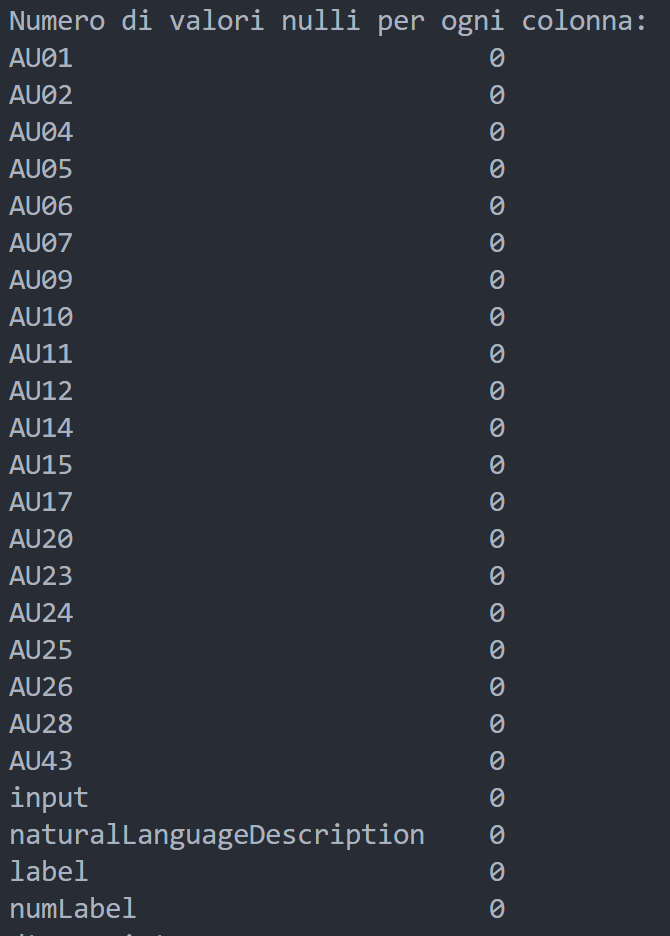
\includegraphics[width=0.6\linewidth]{images/image35.png}
                \caption{Numero di valori nulli ancora presenti nel dataset risultato}
                \label{fig:image8}
            \end{center}
        \end{figure}
        Come è possibile osservare dall’immagine \ref{fig:image8}, il dataset risultato non presenta valori nulli.
    \end{itemize}
    \item aggiunta del valore di frame per ognuna delle analisi dei video:
    \begin{itemize}
        \item ogni analisi dei singoli frame di un video presentava lo stesso percorso di input (il file video associato); di conseguenza ho aggiunto alla fine del valore della colonna di input il frame dal quale sono state estratte le analisi
    \end{itemize}
    \item rimozione delle colonne che non riguardano le Action Units
    \item aggiunta colonne al dataset
    \begin{itemize}
        \item label:
        \begin{itemize}
            \item le analisi inizialmente estrapolate non presentavano già le relative label; è stato quindi opportuno aggiungere
        \end{itemize}
        \item numLabel
        \begin{itemize}
            \item ho associato ad ognuna delle label presenti un numero da 0 a 5:
            \begin{itemize}
                \item 0 $\rightarrow$ confused
                \item 1 $\rightarrow$ engaged
                \item 2 $\rightarrow$ frustrated
                \item 3 $\rightarrow$ bored
                \item 4 $\rightarrow$ drowsy
                \item 5 $\rightarrow$ looking away
            \end{itemize}
        \end{itemize}
        \item descrizione in linguaggio naturale descritta precedentemente
    \end{itemize}
\end{itemize}

\section{Resampling del dataset per migliorare la precisione delle predizioni} 
Il dataset risultato da me realizzato presenta una notevole complicazione: se decidessi di effettuare delle predizioni attraverso uno dei classificatori generati direttamente dal dataset as-his, il numero di campioni (samples) per ognuno dei valori della colonna labels risulterebbe sbilanciato.

Per sbilanciato intendo il fatto che sono presenti molti valori per alcune delle classi (mood), e troppi pochi, a confronto, per altri, come possibile notare nell'immagine \ref{fig:image34}.
\begin{figure}
    \begin{center}    
        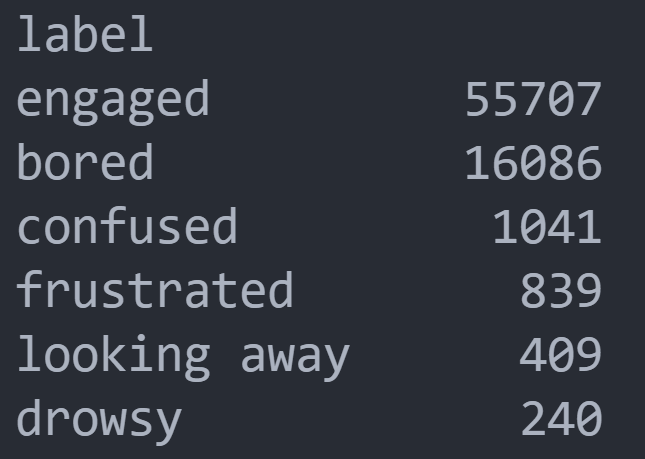
\includegraphics[width=0.2\linewidth]{images/image42.png}
        \caption{Numero di sample per ogni mood nel dataset iniziale}
        \label{fig:image34}
    \end{center}
\end{figure}

Nei grafici \ref{fig:image9} \ref{fig:image10} è possibile riscontrare la differenza fra il numero di elementi per ogni valore unico nella colonna label:
\begin{figure}
    \begin{center}    
        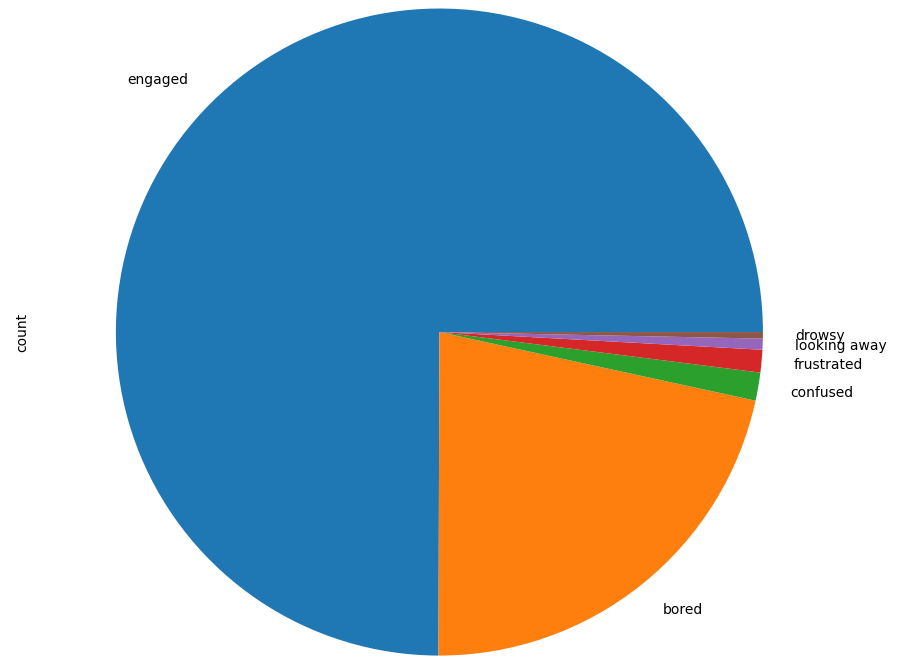
\includegraphics[width=0.75\linewidth]{images/image43.png}
        \caption{Grafico a torta del numero di samples per ogni mood}
        \label{fig:image9}
    \end{center}
\end{figure}
\begin{figure}
    \begin{center}    
        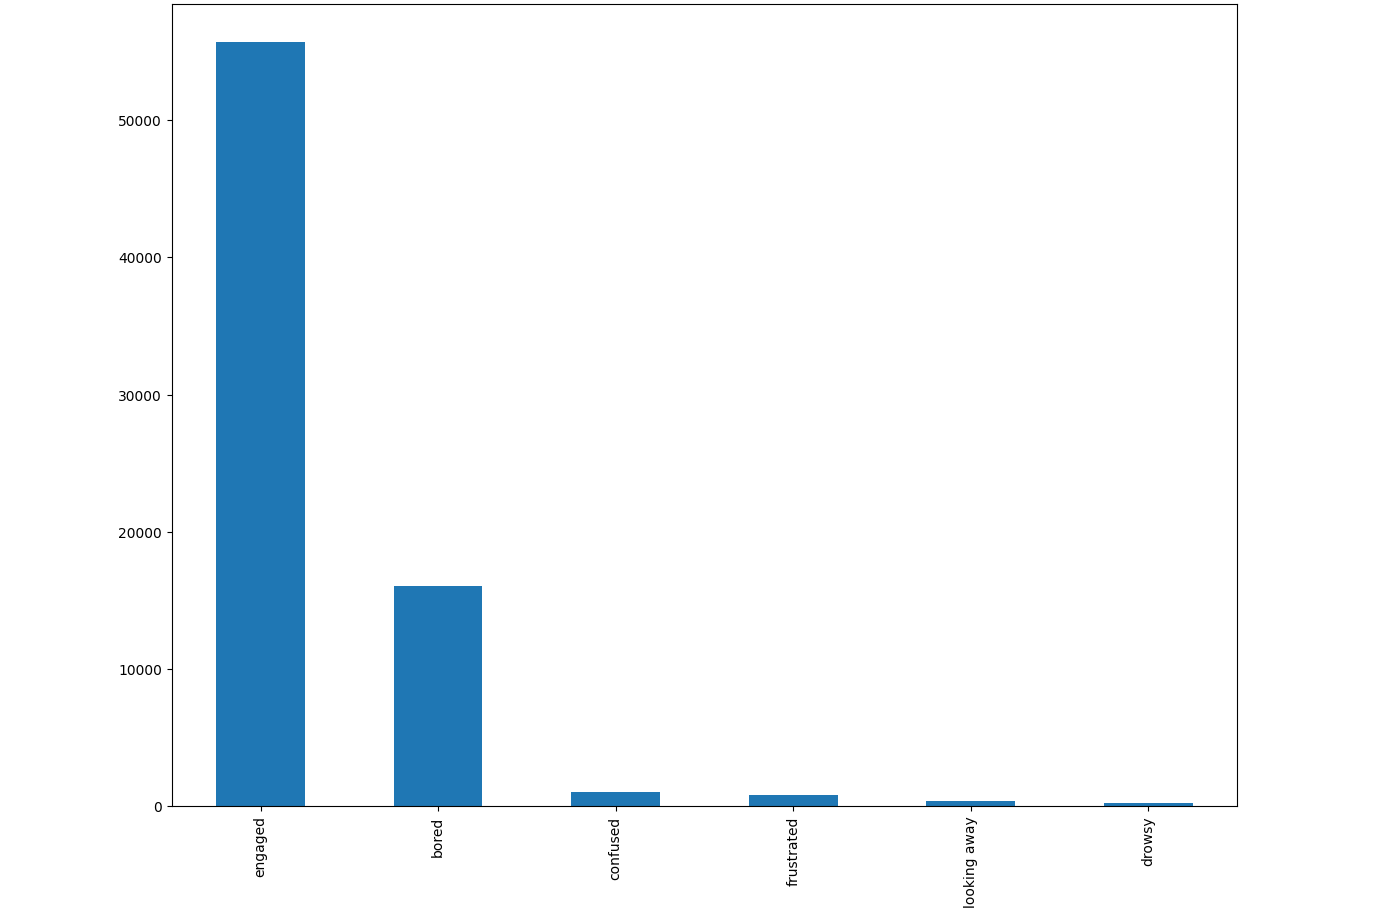
\includegraphics[width=0.75\linewidth]{images/image44.png}
        \caption{Grafico a barre del numero di samples per ogni mood}
        \label{fig:image10}
    \end{center}
\end{figure}

Il resampling, che prevede una modifica  della distribuzione dei dati di un dataset mediante la rimozione o l’aggiunta, in modo casuale, di valori simili a quelli delle sue istanze, è una tecnica comune per bilanciare dataset sbilanciati o per migliorare le prestazioni di modelli di machine learning. Esistono due tipi principali di resampling: undersampling e oversampling:
\begin{itemize}
    \item L'undersampling, come suggerisce il nome, consiste nel rimuovere alcune delle istanze della classe maggioritaria (ovvero quella con un maggior numero di campioni) in modo da bilanciare la distribuzione delle classi nel dataset. 
    
Ciò può essere effettuato in modo casuale, pur essendo possibile utilizzare tecniche più sofisticate, come l'eliminazione degli esempi più vicini (nearest neighbor deletion) o la selezione degli esempi più rappresentativi (prototype selection). 

Il codice utilizzato per effettuare l’undersampling dei sample per ognuna delle labels è il seguente:
\begin{minted}[bgcolor=bg, fontsize=\scriptsize]{python}
import pandas as pd
def undersampleDataset(df, columnName, valueToDownSample, numberOfSamplesAfter):
    if len(df[df[columnName] == valueToDownSample]) > numberOfSamplesAfter:
        engagedIndices = df[df[columnName] == valueToDownSample].index
        tempDf = df.loc[engagedIndices]
        tempDfUndersampled = tempDf.sample(n=numberOfSamplesAfter, random_state=42)
        return pd.concat([df.drop(engagedIndices), tempDfUndersampled])
    return df
\end{minted}
\item L'oversampling, d'altra parte, consiste nell'aumentare il numero di istanze della classe minoritaria (ovvero quella con un minor numero di campioni) in modo da bilanciare la distribuzione delle classi nel dataset.

Sussistono molte tecniche per l'oversampling, tra cui la duplicazione casuale degli esempi esistenti, la generazione di nuovi esempi sintetici attraverso tecniche come la Synthetic Minority Over-sampling Technique (SMOTE), e la duplicazione degli esempi esistenti con una variazione minore (data augmentation). 

Il codice utilizzato per effettuare l’oversampling dei sample per ognuna delle labels è il seguente:
\begin{minted}[bgcolor=bg, fontsize=\scriptsize]{python}
import pandas as pd
from sklearn.utils import resample
def oversampleDataset(df, columnName, valueToOversample, numberOfSamplesAfter):
    if len(df[df[columnName] == valueToOversample]) < numberOfSamplesAfter:
        engagedIndices = df[df[columnName] == valueToOversample].index
        tempDf = df.loc[engagedIndices]
        tempDfOversampled = resample(
            tempDf, 
            replace=True, 
            n_samples=numberOfSamplesAfter, 
            random_state=42
        )
        return pd.concat([df.drop(engagedIndices), tempDfOversampled])
    return df
\end{minted}

\end{itemize}

In sintesi, il resampling è una tecnica utile per bilanciare dataset e migliorare le prestazioni dei modelli di machine learning. 

Questo invece è il codice che gestisce le chiamate per entrambi i metodi riportati sopra:
\begin{minted}[bgcolor=bg, fontsize=\scriptsize]{python}
def resampleDataset ():
    df = pd.read_csv(oldDatasetPath)
    visualizeDataFrameChart(df)

    numberOfValuesForEachLabel = 2000

    labelsList = df["label"].unique()
    for label in labelsList:
        df = undersampleDataset (
            df, 
            "label", 
            label, 
            numberOfValuesForEachLabel
        )
    for label in labelsList:
        df = oversampleDataset (
            df, 
            "label", 
            label, 
            numberOfValuesForEachLabel
        )

   df.to_csv(newDatasetPath, index=False)
\end{minted}


\begin{enumerate}
\item sklearn.utils.resample è una funzione fornita dalla libreria scikit-learn che viene utilizzata al fine di generare esempi sintetici per l'oversampling di dataset. In particolare, la funzione resample prende in input un insieme di campioni e genera un nuovo insieme di campioni sintetici.

La funzione resample prende in input i seguenti parametri:
\begin{itemize}
\item X: un array o un dataframe che rappresenta le feature dei campioni
\item y: (non valorizzato) un array o un dataframe che rappresenta le label dei campioni
\item replace: un valore booleano che indica se l'oversampling deve essere fatto con o senza sostituzione (ovvero se gli esempi sintetici possono essere duplicati)
\item n\_samples: il numero di esempi sintetici da generare
\item random\_state: un valore intero che rappresenta il seed per la generazione casuale degli esempi sintetici
\end{itemize}

La funzione resample restituisce due oggetti:
\begin{itemize}
\item X\_resampled: un array o un dataframe contenente le feature dei campioni originali e dei nuovi esempi sintetici generati (unico output utilizzato)
\item y\_resampled: un array o un dataframe contenente le label dei campioni originali e dei nuovi esempi sintetici generati
\end{itemize}
In sostanza, la funzione resample genera nuovi esempi sintetici aggiungendo variazioni minime ai campioni esistenti, in modo da produrre una distribuzione bilanciata delle classi nel dataset. 

Questi nuovi esempi sintetici vengono poi utilizzati insieme ai campioni esistenti per addestrare i modelli di machine learning.


\item pandas.DataFrame.sample è una funzione fornita dalla libreria pandas che viene utilizzata per estrarre casualmente un sottoinsieme di righe da un dataframe. 

In particolare, la funzione sample prende in input un dataframe e restituisce un nuovo dataframe contenente solo un sottoinsieme delle righe del dataframe originale.
\begin{itemize}
    \item n: il numero di righe da estrarre casualmente
    \item frac: (non valorizzato) la frazione di righe da estrarre casualmente (ad esempio, 0.5 per estrarre il 50% delle righe)
    \item replace: (non valorizzato) un valore booleano che puntualizza se le righe estratte devono essere selezionate con o senza sostituzione (ovvero se una stessa riga può essere selezionata più volte)
    \item weights: (non valorizzato) un array di pesi per ogni riga, utilizzato per selezionare le righe in modo ponderato
    \item random\_state: un valore intero che rappresenta il seed per la generazione casuale degli indici delle righe da selezionare
\end{itemize}
La funzione sample restituisce un nuovo dataframe contenente solo il sottoinsieme delle righe selezionate casualmente dal dataframe originale. 
Fondamentalmente, la funzione sample è utilizzata per ridurre la dimensione del dataframe originale, selezionando solo un sottoinsieme casuale delle righe.
Ciò può dimostrarsi utile per ridurre i tempi di calcolo durante l'addestramento dei modelli di machine learning, in particolare quando il dataset originale è molto ampio e non è necessario utilizzare tutte le righe per ottenere un buon modello.
\end{enumerate}

Per l’appunto, prima di effettuare il resampling del dataset, ho provato ad effettuare delle analisi su nuove immagini utilizzando un classificatore generato dal dataset as-his e i risultati si sono rivelati quelli aspettati, ovvero:

Quasi sempre veniva rilevato che la persona ripresa nell’immagine aveva delle Action Units che portavano alla predizione “engaged” e le altre volte veniva rilevato lo stato d’animo “bored”, ignorando del tutto gli altri valori presenti per la colonna label.

Dopo aver messo in pratica vari test, sono giunto alla conclusione di eseguire un resample al fine di ottenere 2000 istanze per ogni label, in quanto questo sembra il numero di sample in grado di far conseguire risultati più corenti nel tempo; i risultati relativi ottenuti sono riportati nell’ultimo capitolo. 

Di seguito riporto i grafici \ref{fig:image11} e \ref{fig:image12} riguardanti il dataset presentati all’inizio, generati dopo aver effettuato il resampling:
\begin{figure}
    \begin{center}    
        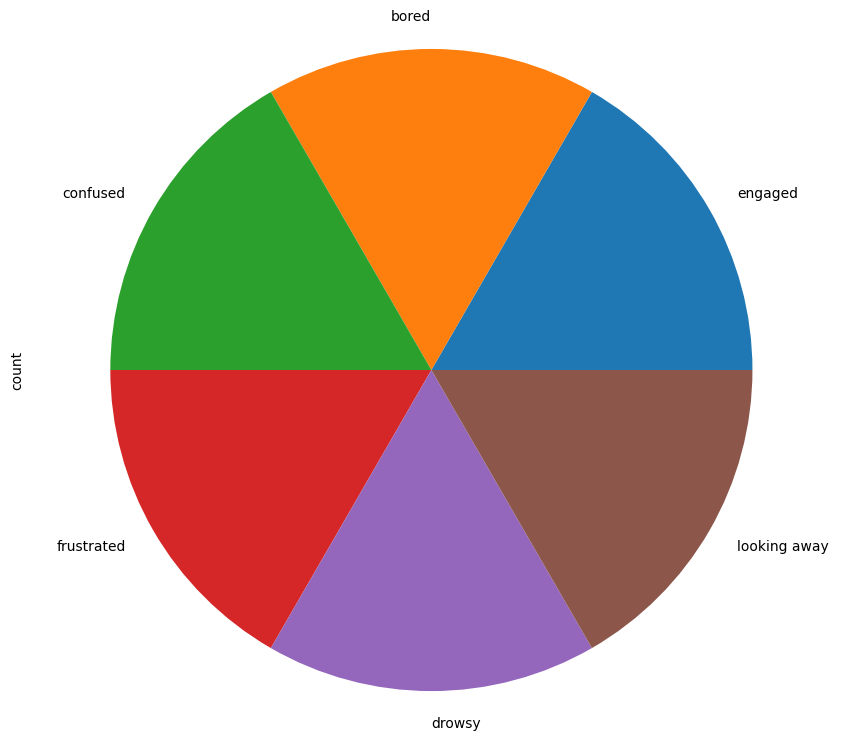
\includegraphics[width=1\linewidth]{images/image45.png}
        \caption{Grafico a torta del numero di samples per ogni mood post resampling}
        \label{fig:image11}
    \end{center}
\end{figure}
\begin{figure}
    \begin{center}    
        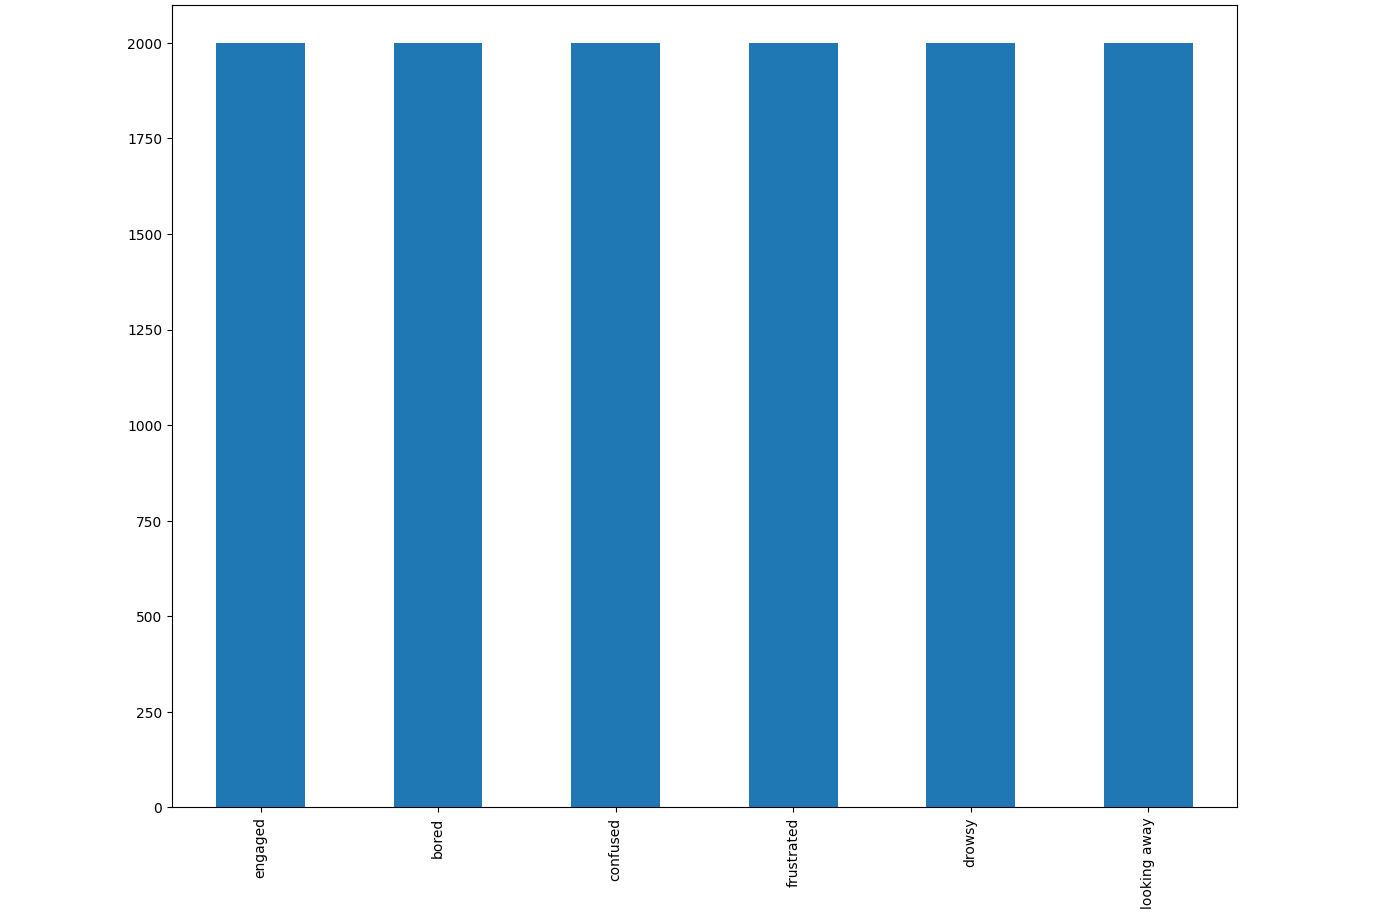
\includegraphics[width=1\linewidth]{images/image46.png}
        \caption{Grafico a barre del numero di samples per ogni mood post resampling}
        \label{fig:image12}
    \end{center}
\end{figure}
\chapter{Modelli predittivi utilizzati}
\section{Algoritmi utilizzati per la creazione dei modelli predittivi}
\subsection{Random forest}
\cite{radnomForestIbm}

\begin{figure}
    \begin{center}    
        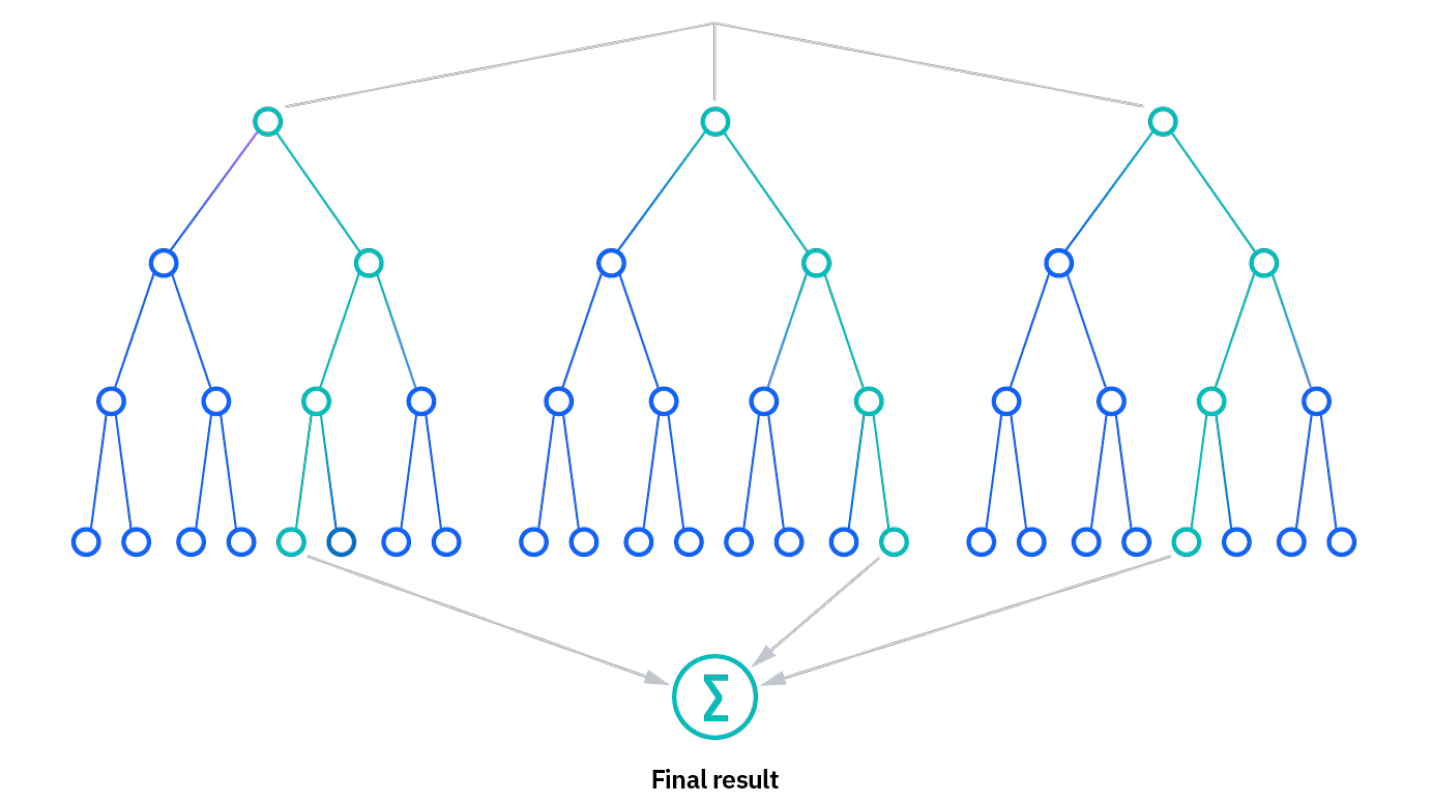
\includegraphics[width=0.9\linewidth]{images/image10.png}
    \end{center}
\end{figure}

La random forest è un algoritmo di apprendimento automatico creato da Leo Breiman e Adele Cutler, che combina l'output di più alberi decisionali col fine di raggiungere un singolo risultato. 

La sua predisposizione intuitiva e la sua flessibilità hanno nutrito l’aumento della sua adozione, in quanto gestisce sia problemi di classificazione che di regressione.

\subsubsection{Alberi decisionali}
Dato che il modello di random forest è composto da più alberi decisionali, è utile descrivere brevemente l'algoritmo dell'albero decisionale. 

Gli alberi decisionali partono da una domanda di base, ad esempio "Dovrei fare surf?". 

A partire da ciò è possibile porre una serie di domande per determinare una risposta, come "C'è un'onda di lungo periodo?" o "Il vento soffia a riva?". 

Queste domande costituiscono i nodi decisionali dell'albero, agendo come mezzo di ripartizione dei dati.

Ogni domanda aiuta l’albero a giungere a una decisione finale, indicata dal nodo foglia raggiunto. 

Le osservazioni che soddisfano i criteri seguiranno il ramo "Sì", mentre quelle che non li soddisfano seguiranno il percorso alternativo. 

Gli alberi decisionali cercano di trovare la miglior suddivisione per i dati, e vengono tipicamente addestrati attraverso l'algoritmo Classification and Regression Tree (CART). 

Metriche come l'impurità di Gini, il guadagno di informazione o l'errore quadratico medio (MSE) possono essere utilizzati per valutare la qualità della suddivisione.

Sebbene gli alberi decisionali siano comuni algoritmi di apprendimento supervisionato, possono essere soggetti a problemi come il bias e l'overfitting. 

Tuttavia, quando più alberi decisionali formano un insieme nell'algoritmo di random forest, predicono risultati più accurati, in particolar modo quando i singoli alberi non sono correlati tra loro.

\subsubsection{L'algoritmo della random forest}
L'algoritmo della random forest è un'estensione del metodo di bagging, in quanto utilizza sia il bagging che la casualità delle features per creare una foresta di alberi decisionali non correlati. 

La casualità delle features, altrimenti nota come bagging delle caratteristiche o "metodo del sottospazio casuale", genera un sottoinsieme casuale di caratteristiche che assicura una bassa correlazione tra gli alberi decisionali. 

Questa è una differenza chiave tra gli alberi decisionali e le random forest, poiché mentre gli alberi decisionali considerano tutte le possibili suddivisioni delle caratteristiche, le random forest selezionano solo un sottoinsieme di quelle caratteristiche.

Tornando all'esempio "dovrei fare surf?", le domande che potrei porre per determinare la previsione potrebbero non essere così esaustive come il set di domande di un altro utente. 

Tenendo conto di tutta la potenziale variabilità dei dati, possiamo ridurre il rischio di overfitting, di bias e di varianza complessiva, ottenendo previsioni via via più precise.

\subsubsection{Come funziona}
Gli algoritmi delle random forest hanno tre iperparametri principali da impostare prima dell'allenamento. 
Questi includono: 

\begin{itemize}
  \item la dimensione del nodo, 
  \item il numero di alberi, 
  \item il numero di caratteristiche campionate
\end{itemize}

Da lì, il classificatore della random forest può essere utilizzato per risolvere problemi di regressione o di classificazione.

L'algoritmo della random forest è costituito da una collezione di alberi decisionali, dove ogni albero nell'insieme è costituito da un campione di dati tratto da un set di allenamento con sostituzione, chiamato campione di bootstrap. 

Di quel campione di allenamento, ad esempio, un terzo viene messo da parte come dati di test, noti come campione fuori dalla borsa (oob), su cui ci soffermeremo in seguito. 

Un'altra istanza di casualità viene quindi iniettata attraverso il bagging delle caratteristiche, incrementando la diversità nel dataset e riducendo la correlazione tra gli alberi decisionali. 

A seconda del tipo di problema, la determinazione della previsione subirà variazioni; per un compito di regressione gli alberi decisionali individuali verranno mediati, mentre per un compito di classificazione una maggioranza di voti, ossia la variabile categorica più frequente, darà come risultato la classe prevista. 

Infine, il campione oob viene utilizzato per la convalida incrociata, finalizzando quella previsione.

\subsubsection{Benefici e sfide del random forest}
Ci sono diversi vantaggi e sfide che l'algoritmo random forest presenta quando utilizzato per problemi di classificazione o regressione. Alcuni di essi includono:

\begin{itemize}
  \item Principali vantaggi
  \begin{itemize}
    \item Riduzione del rischio di overfitting: gli alberi di decisione corrono il rischio di overfitting poiché tendono ad adattarsi strettamente a tutti i campioni all'interno dei dati di formazione. 
    Tuttavia, quando è presente un largo numero di alberi di decisione in un random forest, il classificatore non sovrastimerà il modello, poiché la media di alberi non correlati fra loro riduce la variazione complessiva e l'errore di previsione.
    \item Flessibilità: il random forest può gestire sia compiti di regressione che di classificazione con un elevato grado di precisione, distinguendosi in quanto metodo popolare tra i data scientist. 
    Inoltre, la feature bagging rende il classificatore random forest uno strumento adeguato per la stima dei valori mancanti, in quanto mantiene l'accuratezza quando una parte dei dati è irreperibile.
    \item Facile determinazione dell'importanza delle feature: il random forest rende facile valutare l'importanza delle variabili, o del contributo, al modello. 
    Sussistono alcuni modi per valutare l'importanza della feature; l’importanza di Gini e la diminuzione media dell'impurità (MDI) vengono solitamente utilizzati per misurare quanto diminuisce l'accuratezza del modello quando una determinata variabile viene esclusa.
  \end{itemize}
  \item Principali sfide
  \begin{itemize}
    \item È un processo che richiede tempo: gli algoritmi random forest possono gestire grandi set di dati e fornire previsioni più accurate; tuttavia il processo è rallentato dalla computazione dei dati per ogni singolo albero decisionale.
    \item Richiede più risorse: le random forest, elaborando set di dati più grandi, richiedono più risorse per archiviare questi ultimi.
    \item Più complesso: la previsione di un singolo albero decisionale è più facile da interpretare rispetto a una foresta di questi.
  \end{itemize}
\end{itemize}


\subsection{K-nearest neighbors}
\cite{KNNibm}

\begin{figure}
    \begin{center}    
        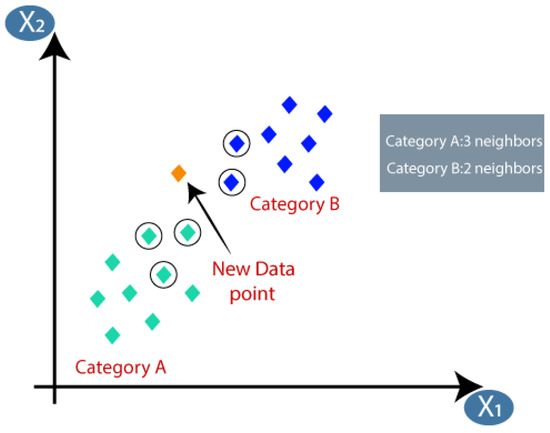
\includegraphics[width=0.9\linewidth]{images/image11.jpeg}
    \end{center}
\end{figure}

L'algoritmo k-nearest neighbors, noto anche come KNN o k-NN, è un classificatore di apprendimento supervisionato non parametrico.

Esso sfrutta la prossimità per effettuare classificazioni o previsioni sul raggruppamento di un singolo punto dati. 

Sebbene possa essere utilizzato per problemi di regressione o classificazione, viene generalmente impiegato in quanto algoritmo di classificazione, basandosi sul presupposto che dati simili, se analizzati o rappresentati nella giusta maniera, possono essere trovati l'uno vicino all'altro.

Per i problemi di classificazione un'etichetta di classe viene assegnata sulla base di un voto a maggioranza(ad es. viene utilizzata l'etichetta più frequentemente rappresentata attorno a un determinato punto dati).

I problemi di regressione utilizzano un concetto simile al problema di classificazione; in questo caso però viene presa la media dei k elementi vicini più vicini per effettuare una previsione su una classificazione. 

Qui, ciò che si discosta notevolmente, è il fatto che la classificazione viene utilizzata per i valori discreti, mentre la regressione viene utilizzata per quelli continui. 

Tuttavia, prima di poter effettuare una classificazione, è necessario definire il concetto di distanza. 

La distanza euclidea, altra metrica di distanza popolare, misura il valore assoluto tra due punti.

Vale la pena notare che l'algoritmo KNN fa anche parte di una famiglia di modelli di "apprendimento pigro", il che significa che memorizza solo un set di dati di addestramento nella fase di addestramento. 

Perviene quindi che tutto il calcolo avvenga quando si compie una classificazione o una previsione. 

Poiché fa ampiamente affidamento sulla memoria per archiviare tutti i suoi dati di addestramento, viene anche definito metodo di apprendimento basato su istanze o basato sulla memoria.

Le idee iniziali sul modello KNN sono attribuite a Evelyn Fix e Joseph Hodges in questo articolo \cite{KNNEvelynFixJosephHodges} del 1951, mentre Thomas Cover ne amplia il concetto nella sua ricerca, “Nearest Neighbor Pattern Classification”\cite{NearNeighPattClass}.

Pur non riscuotendo un tale successo come in precedenza, è ancora uno dei primi algoritmi che si affronta nello studio della data science per la sua semplicità ed accuratezza. 

Tuttavia, al crescere di un set di dati KNN diventa sempre più inefficiente, compromettendo le prestazioni del modello. 

Viene riscontrato il suo impiego per semplici sistemi di raccomandazione, riconoscimento di modelli, data mining, previsioni dei mercati finanziari, rilevamento delle intrusioni e altro ancora. 

\subsubsection{Calcolare il KNN: metriche di distanza}
Ricapitolando, l'obiettivo dell'algoritmo k-nearest neighbor è identificare i vicini più prossimi di un dato punto di query, in modo da poter assegnare un'etichetta di classe a quel punto. 

Per determinare quali punti dati sono più attigui ad un determinato punto di query, sarà necessario calcolare la distanza tra il punto di interrogazione e gli altri punti dati. 

Le metriche di distanza aiutano a formare confini decisionali che suddividono i punti di query in regioni diverse. 

Sebbene sussistano diverse misure di distanza, tra cui è possibile scegliere, l’articolo sul sito di IBM tratta esclusivamente quelle a seguire:
\begin{itemize}
    \item Distanza euclidea (p=2): la misura della distanza più comunemente adottata; essa è limitata ai vettori con valori reali. 
    
    Utilizzando la formula seguente traccia una linea retta tra il punto di query e l'altro punto che si vuole misurare.
    \begin{figure}
        \begin{center}    
            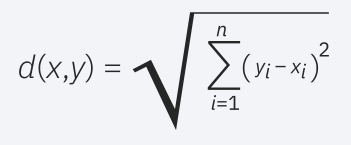
\includegraphics[width=0.45\linewidth]{images/image12.png}
        \end{center}
    \end{figure}
    \item Distanza di Manhattan (p=1): un'altra metrica di distanza particolarmente nota che si propone di misurare il valore assoluto tra due punti. 
    
    È anche riconosciuta come distanza del taxi o distanza del blocco cittadino, poiché è comunemente visualizzata con una griglia che illustra come si potrebbe percorrere il tragitto da un indirizzo all'altro attraverso le strade della città.
    \begin{figure}
        \begin{center}    
            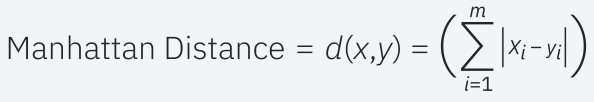
\includegraphics[width=0.45\linewidth]{images/image13.png}
        \end{center}
    \end{figure}
    \item Distanza di Minkowski: questa misura della distanza è la forma generalizzata delle metriche di distanza euclidea e di Manhattan. Il parametro, p, nella formula seguente, consente la creazione di altre metriche di distanza.    
    
    La distanza Euclidea è rappresentata da questa formula quando p è uguale a due e la distanza di Manhattan è indicata con p uguale a uno.

    \begin{figure}
        \begin{center}    
            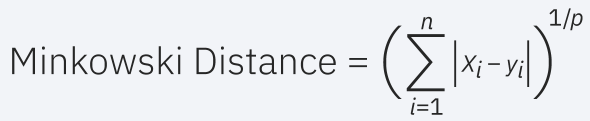
\includegraphics[width=0.45\linewidth]{images/image14.png}
        \end{center}
    \end{figure}
    \item Distanza di Hamming: questa tecnica viene utilizzata tipicamente con vettori booleani o stringa, identificando i punti in cui i vettori non trovano corrispondenza. 
    
    Di conseguenza, è stata anche definita metrica di sovrapposizione.
    \begin{center}    
        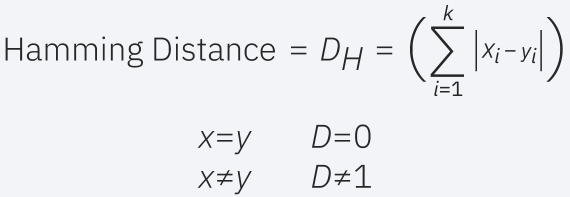
\includegraphics[width=0.45\linewidth]{images/image15.png}
    \end{center}
    
\end{itemize}


Ad esempio, se avessi le seguenti stringhe, la distanza di Hamming sarebbe due poiché solo due dei valori differiscono.
\begin{center}    
    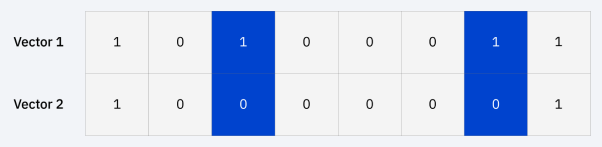
\includegraphics[width=0.8\linewidth]{images/image16.png}
\end{center}


\subsubsection{Calcolare KNN: definizione di k}
Il valore k nell'algoritmo k-NN definisce quanti vicini verranno controllati per determinare la classificazione di un punto di query specifico. 

Di fatti, se k=1, l'istanza verrà assegnata alla stessa classe del suo singolo neighbors più vicino. 

Definire k può essere un atto di bilanciamento, in quanto valori diversi possono portare a overfitting o underfitting. 

Valori inferiori a k possono essere caratterizzati da una variabilità elevata ma una bassa distorsione, mentre valori maggiori di k possono portare a una distorsione elevata e una variabilità inferiore. 

La scelta di k dipenderà in particolar modo dai dati di input, dal momento che i dati con più valori anomali o rumore probabilmente opereranno in modo più proficuo tanto più elevati sono i valori di k. 

In generale si consiglia di adoperare un numero dispari per k, col fine di evitare pareggi nella classificazione.

\subsubsection{Applicazioni di k-NN nell'apprendimento automatico}
L'algoritmo k-NN è stato utilizzato all'interno di una varietà di applicazioni, in maggior misura all'interno della classificazione. Alcuni di questi casi d'uso includono:
\begin{itemize}
\item Pre-elaborazione dei dati: poichè i dataset presentano spesso valori mancanti, l'algoritmo KNN può stimare tali valori in un processo noto come imputazione dei dati mancanti.
\item Recommender systems: adoperando i dati del flusso di clic dai siti web, l'algoritmo KNN è stato utilizzato per fornire consigli automatici agli utenti su contenuti aggiuntivi. Da tale ricerca emerge che un utente è assegnato a un particolare gruppo e, sulla base del comportamento di quest'ultimo, riceve un consiglio. Tuttavia, dati i problemi di scalabilità con KNN, questo approccio potrebbe non risultare ottimale in caso di impiego di dataset più grandi.
\item Finanza: è stato utilizzato anche in una varietà di casi di utilizzo finanziari ed economici. Ipoteticamente, un articolo mostra in che modo l'utilizzo di KNN sui dati di credito può aiutare le banche nella valutazione dei rischi su un prestito a un'organizzazione o a un individuo. Viene quindi sfruttato per determinare l'affidabilità creditizia del richiedente di tale prestito. Un altro articolo ne sottolinea l'uso nelle previsioni del mercato azionario, nei tassi di cambio, nel trading di fetures e nelle analisi sul riciclaggio di denaro.
\item Assistenza sanitaria: KNN ha riscontrato applicazioni anche nel settore dell'assistenza sanitaria, effettuando previsioni sul rischio di infarto e cancro alla prostata. L'algoritmo funziona calcolando le espressioni geniche più probabili.
\item Riconoscimento dei pattern: KNN ha anche aiutato a identificare i pattern, come nel testo e nella classificazione digitale. Ciò è stato particolarmente utile per identificare i numeri scritti a mano in cui ci si potrebbe imbattere su moduli o buste postali.
\end{itemize}
\subsubsection{Vantaggi e svantaggi dell'algoritmo KNN}
K-NN possiede i suoi punti di forza e di debolezza. A seconda del progetto e dell'applicazione, potrebbe rivelarsi o meno la scelta giusta.
\begin{itemize}
\item Vantaggi
\begin{itemize}
\item Facile da implementare: data la semplicità e l'accuratezza dell'algoritmo, è uno dei primi classificatori che un data scientist alle prime armi apprenderà.
\item Si adatta facilmente all'aggiunta di nuovi campioni di addestramento, l'algoritmo si adatta per tenere conto di eventuali nuovi dati, a fronte dell'archivio di tutti i dati di addestramento in memoria.
\item Pochi iperparametri: KNN necessita solo di un valore k e una metrica di distanza, il che, a confronto con altri algoritmi di machine learning, è minore in quantità.
\end{itemize}
\item Svantaggi
\begin{itemize}
\item Non è provvisto di una buona scalabilità: essendo KNN un algoritmo cosiddetto pigro, occupa più memoria e spazio di storage dei dati rispetto ad altri classificatori.
Sebbene diverse strutture di dati ,come Ball-Tree, siano state create per affrontare le inefficienze computazionali, un classificatore diverso potrebbe dimostrarsi ideale.
\item Maledizione della dimensionalità: l'algoritmo tende a cadere vittima della “maledizione della dimensionalità”; ciò significa che non ricopre adeguatamente il proprio ruolo con input di dati ad alta dimensionalità.
Questo è a volte indicato anche come il fenomeno del picco, nel quale, dopo che l'algoritmo raggiunge l'ottimale numero di funzioni, le funzioni aggiuntive aumentano la quantità di errori di classificazione, soprattutto quando la dimensione del campione è inferiore.
\item Propensione al sovradimensionamento dei dati: a causa della "maledizione della dimensionalità", KNN è anche più propenso al sovradimensionamento dei dati.
Sebbene le tecniche di selezione delle caratteristiche e di riduzione della dimensionalità vengano sfruttate per evitare che ciò accada, il valore di k può inevitabilmente influire sul comportamento del modello.
Valori più bassi di k possono sovra-alimentare i dati, mentre valori più alti di k tendono a "smussare" i valori di previsione, poiché si sta attuando la media dei valori su un'area o un neighborhood più grande.
Tuttavia, se il valore di k è troppo alto, può essere inferiore ai dati.
\end{itemize}
\end{itemize}

\subsection{Naive Bayes Classifier}
\cite{NaiveBayesClassTowardDataScience}
Un classificatore di Bayes è un modello di apprendimento automatico probabilistico utilizzato per compiti di classificazione. Il fulcro del classificatore si basa sul teorema di Bayes.


\subsubsection{Teorema di Bayes}
Utilizzando il teorema di Bayes, possiamo trovare la probabilità che A accada, conseguentemente all’avvenimento di B. Qui, B è la prova e A è l'ipotesi. 

L'assunzione alla base del teorema è che i predittori e le caratteristiche siano indipendenti: in altre parole, la presenza di una particolare caratteristica non influisce sull'altra.
\begin{figure}
    \begin{center}    
        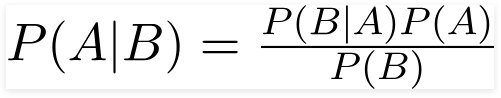
\includegraphics[width=0.9\linewidth]{images/image17.png}
    \end{center}
\end{figure}
Volendo offrire un esempio al fine di una migliore comprensione, consideriamo il problema di giocare a golf.  Il dataset è rappresentato come segue.
\newpage
\begin{figure}
    \begin{center}    
        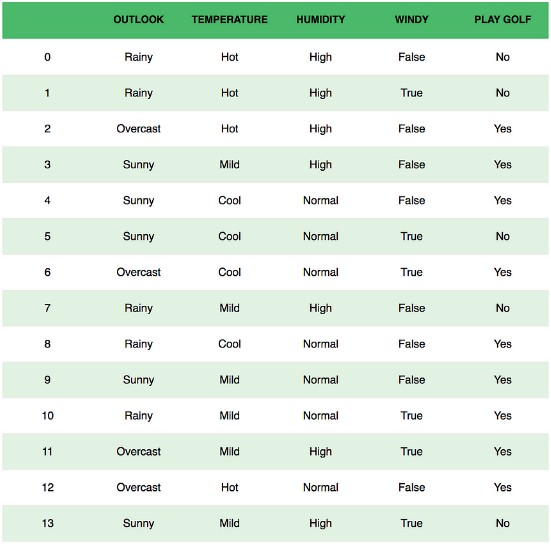
\includegraphics[width=0.9\linewidth]{images/image18.jpeg}
    \end{center}
\end{figure}
Classifichiamo se la giornata si configura adatta per una partita di golf, basandoci sugli attributi di tale giornata. Le colonne rappresentano questi attributi, mentre le righe rappresentano le singole voci.

Prendendo a campione la prima riga del dataset, possiamo osservare che non è adatta per giocare a golf se il cielo è nuvoloso, la temperatura è calda, l'umidità è alta e non c'è vento. Qui facciamo due assunzioni: 

come già detto, consideriamo che questi predittori siano indipendenti (ovvero, se la temperatura è calda, non significa necessariamente che l'umidità sia alta). Un'altra assunzione fatta qui è che tutti i predittori abbiano un effetto uguale sul risultato. Cioè, il fatto che ci sia vento non ha una maggiore importanza nella  decisione di giocare a golf o meno. 

Rifacendosi al secondo esempio, il teorema di Bayes può essere quindi riscritto come segue:
\newpage
\begin{figure}
    \begin{center}    
        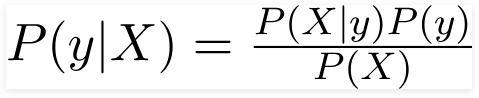
\includegraphics[width=0.8\linewidth]{images/image19.png}
    \end{center}
\end{figure}
La variabile y è la variabile di classe (giocare a golf), la quale rappresenta quanto sia adatta la giornata o meno per giocare a golf. La variabile X rappresenta i parametri/caratteristiche.

X è dato come segue:
\begin{center}    
    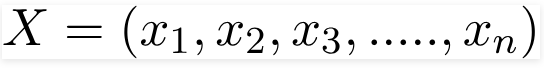
\includegraphics[width=0.9\linewidth]{images/image20.png}
\end{center}


Qui x1, x2... xn raffigurano le caratteristiche, cioè possono essere mappati su cielo, temperatura, umidità e vento. Sostituendo X ed espandendo utilizzando la regola della catena otteniamo:
\begin{figure}
    \begin{center}    
        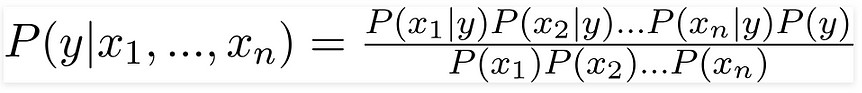
\includegraphics[width=0.9\linewidth]{images/image21.jpeg}
    \end{center}
\end{figure}

Ora è possibile ottenere i valori per ognuno guardando il dataset e sostituendoli nell'equazione. Per tutte le voci nel dataset, il denominatore non cambia, rimane statico. Pertanto, il denominatore può essere rimosso e può essere introdotta una proporzionalità.
\begin{center}    
    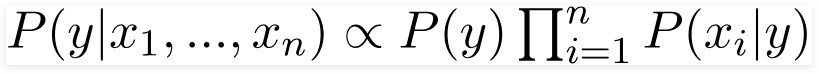
\includegraphics[width=0.9\linewidth]{images/image22.jpeg}
\end{center}


Nel nostro caso, la variabile di classe (y) ha solo due risultati, sì o no. Potrebbero esserci casi in cui la classificazione potrebbe rivelarsi multivariata. Pertanto, sarà necessario trovare la classe y con la massima probabilità.
\begin{center}    
    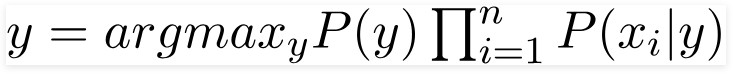
\includegraphics[width=0.5\linewidth]{images/image23.jpeg}
\end{center}

Utilizzando questa funzione ci è possibile ottenere la classe, dato il predittore.




\subsubsection{Tipi di Classificatori Bayesiani}
\begin{itemize}
\item Classificatore Bayesiano Multinomiale:
\begin{itemize}
\item Esso è principalmente utilizzato per problemi di classificazione dei documenti; ad esempio, se un documento appartiene alla categoria di sport, politica, tecnologia, ecc. Le caratteristiche/predittori impiegati dal classificatore saranno la frequenza delle parole presenti nel documento.
\end{itemize}
\item Classificatore Bayesiano di Bernoulli:
\begin{itemize}
\item Questo classificatore è simile al precedentemente citato, pur essendo i predittori variabili booleane. I parametri che usiamo per prevedere la variabile di classe assumono solo valori sì o no (se una parola compare nel testo o meno).
\end{itemize}
\item Classificatore Bayesiano Gaussiano:
\begin{itemize}
\item Quando i predittori assumono un valore continuo e non discreto, assumiamo che questi valori siano estratti da una distribuzione gaussiana.
\end{itemize}
\end{itemize}
Poiché il modo in cui i valori sono presenti nel dataset cambia, la formula per la probabilità condizionata cambia in questo caso,
\begin{figure}
    \begin{center}    
        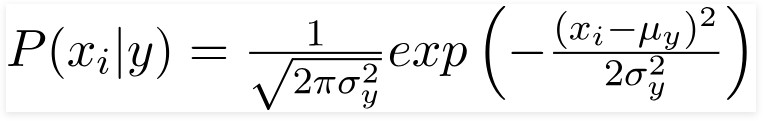
\includegraphics[width=1\linewidth]{images/image24.jpeg}
    \end{center}
\end{figure}

\subsubsection{Conclusione}
Gli algoritmi Bayesiani sono principalmente utilizzati nell'analisi del sentiment, nel filtraggio dello spam, nei reccomender systems, ecc. 

Sono veloci e facili da implementare, ma il loro più grande svantaggio è la necessità che i predittori siano indipendenti. 

Nella maggior parte dei casi reali, i predittori sono dipendenti, il che ostacola le prestazioni del classificatore.


\subsection{Support Vector Machine}
Il support vector machine è favorito maggiormente data la produzione di una significativa accuratezza mediante una minor potenza di calcolo. 

Il Support Vector Machine, abbreviato come SVM, può essere utilizzato sia per compiti di regressione che di classificazione. Tuttavia, viene ampiamente sfruttato negli obiettivi di classificazione.
\subsubsection{Cosa è il Support Vector Machine?}
L'obiettivo dell'algoritmo support vector machine è quello di trovare un iperpiano in uno spazio N- dimensionale (N - il numero di caratteristiche) che classifichi distintamente i punti dati.
\begin{figure}[h]
  \begin{minipage}[b]{0.45\linewidth}
    \centering
    \includegraphics[width=\linewidth]{images/image25.png}
  \end{minipage}
  \begin{minipage}[b]{0.45\linewidth}
    \centering
    \includegraphics[width=\linewidth]{images/image26.png}
  \end{minipage}
\end{figure}

Per separare le due classi di punti dati sono presenti molti iperpiani possibili da cui poter scegliere. Il nostro obiettivo è trovare un piano che possegga il margine massimo, ovvero la massima distanza tra i punti dati di entrambe le classi. Massimizzare la distanza del margine fornisce un rinforzo in modo che i futuri punti dati possano essere classificati con maggiore fiducia.

\subsubsection{Iperpiani e support vector}
Gli iperpiani sono i confini decisionali che aiutano a classificare i punti dati. 

I punti dati che cadono su entrambi i lati dell'iperpiano possono essere attribuiti a diverse classi. 

Inoltre, la dimensione dell’iperpiano  dipende dal numero di caratteristiche. 

\begin{figure}
    \begin{center}    
        \includegraphics[width=0.9\linewidth]{images/image27.jpeg}
    \end{center}
\end{figure}

\newpage
Se il numero di caratteristiche di input è 2, l'iperpiano è solo una linea. Se il numero di caratteristiche di input è 3, l'iperpiano diventa un piano bidimensionale. Diventa difficile immaginare quando il numero di caratteristiche supera 3.
\begin{figure}
    \begin{center}    
        \includegraphics[width=0.9\linewidth]{images/image28.jpeg}
    \end{center}
\end{figure}

I support vector sono i punti dati più vicini all'iperpiano e influenzano la posizione e l'orientamento di quest’ultimo. Impiegando i support vector, massimizziamo il margine del classificatore. L’eliminazione  dei support vector cambierà la posizione dell'iperpiano. 

\subsubsection{Intuizione del grande margine}
Nella regressione logistica, prendiamo l'output della funzione lineare e normalizziamo il valore nell'intervallo  [0,1] utilizzando la funzione sigmoide. 

Se il valore normalizzato è maggiore di un valore soglia (0,5), gli assegniamo una etichetta 1, altrimenti gli assegniamo un'etichetta 0. 

Nell'SVM, prendiamo l'output della funzione lineare e, se quell'output è maggiore di 1, lo identifichiamo con una classe, mentre se l'output è -1, lo identifichiamo con un'altra classe. 

Poiché i valori della soglia sono cambiati in 1 e -1 nell'SVM, otteniamo questo intervallo ([-1,1]) che viene utilizzato come margine.


\subsubsection{Funzione di costo e aggiornamenti del gradiente}
Nell'algoritmo SVM, cerchiamo di massimizzare la distanza tra i punti dati e l'iperpiano. La funzione di perdita che ci aiuta a massimizzare la distanza è la hinge loss.
\begin{figure}[h]
  \begin{minipage}[b]{0.45\linewidth}
    \centering
    \includegraphics[width=\linewidth]{images/image29.jpeg}
  \end{minipage}
  \begin{minipage}[b]{0.45\linewidth}
    \centering
    \includegraphics[width=\linewidth]{images/image30.jpeg}
  \end{minipage}
\end{figure}

Il costo è 0 se il valore previsto e il valore effettivo hanno lo stesso segno. In caso contrario, calcoliamo il valore di perdita. Aggiungiamo anche un parametro di regolarizzazione alla funzione di costo. L'obiettivo del
parametro di regolarizzazione è di bilanciare la massimizzazione della distanza con la perdita. 

Dopo aver aggiunto il parametro di regolarizzazione, la funzione di costo appare come segue.
\begin{figure}
    \begin{center}    
        \includegraphics[width=0.9\linewidth]{images/image31.jpeg}
    \end{center}
\end{figure}

Ora che abbiamo ottenuto la funzione di perdita, utilizziamo le derivate parziali rispetto ai pesi per trovare i gradienti. 

Così facendo, possiamo aggiornare i pesi.
\begin{center}    
    \includegraphics[width=0.9\linewidth]{images/image32.jpeg}
\end{center}

Quando non vi è alcuna errata classificazione, ovvero il nostro modello prevede correttamente la classe del nostro punto dati, sarà necessario aggiornare solo il gradiente dal parametro di regolarizzazione.
\begin{figure}
    \begin{center}    
        \includegraphics[width=0.5\linewidth]{images/image33.png}
    \end{center}
\end{figure}

Quando ci si trova di fronte ad una errata classificazione, ossia il nostro modello commette un errore sulla previsione della classe del nostro punto dati, includiamo la perdita insieme al parametro di regolarizzazione per eseguire l'aggiornamento del gradiente.
\begin{figure}
    \begin{center}    
        \includegraphics[width=0.5\linewidth]{images/image34.png}
    \end{center}
\end{figure}

\section{Random forest classifier}
Per effettuare delle predizioni sul dataset ho realizzato un classificatore random forest sul quale effettuare delle query, fornendogli i dati riguardanti le Action Units da nuove immagini, sempre attraverso la libreria py-feat.

Per la creazione del classificatore ho in primis letto il file csv contenente il dataset pre-elaborato (modifiche precedentemente trattate e sulle quali aggiungerò considerazioni, in quanto è risultato efficace applicarne ulteriori per migliorare la precisione del predittore creato), rimosso le colonne non necessarie e, infine, ho diviso il dataset in set di addestramento e di test usando la funzione train\_test\_split della libreria sklearn.model\_selection; tramite l’output di questo metodo ho ricavato i pandas’s dataframes Xtrain, Xtest, yTrain, yTest.

Questo è il metodo relativo:
\begin{minted}[bgcolor=bg]{python}
def getXtrainYTrainXtestYTest():
    pd.read_csv(join(dirname(
            abspath(__file__)), 
            "../final analysis/" + 
            "DAiSEE and student engagement dataset clean sampled.csv"
        )
    )
    y = df['label']
    X = df.drop(
        ["input","naturalLanguageDescription","label","numLabel"], 
        axis=1
    )
    
    Xtrain, Xtest, yTrain, yTest = train_test_split(
        X, 
        y, 
        test_size=0.2, 
        random_state=69
    )

    return Xtrain, yTrain 
\end{minted}
Una volta ottenuti questi dataset ho creato il classificatore utilizzando l’oggetto a disposizione fornito dalla libreria sklearn.ensable.

Il RandomForestClassifier viene generato con 100 alberi di decisione e viene addestrato con l’utilizzo dei due dataframe Xtrain e yTrain restituiti dalla funzione getXtrainYTrainXtestYTest().

Il metodo è il seguente:
\begin{minted}[bgcolor=bg]{python}
randomForestClassifier = RandomForestClassifier(
    n_estimators=100, 
    verbose=True, 
    random_state=69
)
Xtrain, yTrain = getXtrainYTrainXtestYTest ()
randomForestClassifier.fit(Xtrain, yTrain)
return randomForestClassifier
\end{minted}

Eseguendo dei test attraverso il metodo \mintinline[bgcolor=bg]{python}{score(Xtest, yTest)} offerto dal random forest classifier generato dalla libreria sklearn.ensemble ho potuto calcolare l’accuracy del modello da me generato.

I risultati di questa analisi sono che il random forest classifier ottiene una precisione dell’82,3periodico\% sul dataset di test generato nel metodo \mintinline[bgcolor=bg]{python}{getXtrainYTrainXtestYTest}

\begin{figure}
    \begin{center}    
        \includegraphics[width=0.9\linewidth]{images/image36.png}
    \end{center}
\end{figure}

Oltre alla produzione del classificatore viene anche generato un grafico per la visualizzazione dell’influenza di ognuna delle label sulla predizione che allego qui di seguito:
\newpage
\begin{figure}
    \begin{center}    
        \includegraphics[width=1\linewidth]{images/image37.png}
    \end{center}
\end{figure}

Come è possibile constatare, quasi tutte le label influenzano la predizione in modo simile (in un range fra il 7,2\% e l’11,9\%) tranne per la AU43 (Eyes Closed) che, ovviamente, influenza largamente la predizione effettuata dal modello.

\section{K-nearest Neighbors Classifier}
Un ulteriore classificatore realizzato per effettuare predizioni sul dataset è il K-nearest Neighbors Classifier, attraverso il quale ho effettuato delle query fornendo i dati delle Action Units da nuove immagini.

Come per il random forest classifier, per la creazione del classificatore ho in primis letto il file csv contenente il dataset pre-elaborato, rimosso le colonne non necessarie e, infine, ho diviso il dataset in set di addestramento e di test usando la funzione train\_test\_split della libreria sklearn.model\_selection; tramite l’output di questo metodo ho ricavato i pandas’s dataframes Xtrain, Xtest, yTrain, yTest.

Il metodo sopracitato per l’estrazione di questi dataframe è lo stesso riportato in pochi paragrafi precedenti.

Una volta ottenuti questi dataset ho creato il classificatore utilizzando l’oggetto a disposizione fornito dalla libreria sklearn.neighbors.

Il K-nearest Neighbors Classifier viene creato impostando il parametro relativo al numero di elementi vicini da utilizzare settato a 1 e viene addestrato con l’utilizzo dei due dataframe Xtrain e yTrain restituiti dalla funzione getXtrainYTrainXtestYTest().

Il metodo è il seguente
\begin{minted}[bgcolor=bg]{python}
KnnClassifier = KNeighborsClassifier(n_neighbors=1)
Xtrain, yTrain = getXtrainYTrainXtestYTest ()
KnnClassifier.fit(Xtrain, yTrain)
return KnnClassifier
\end{minted}

Ho ritenuto opportuno valorizzare il campo con 1, in quanto è risultato il quantitativo necessario per non ottenere delle rilevazioni “ballerine” all’interno dell’interfaccia grafica da me realizzata e, allo stesso tempo, avere il miglior valore di accuracy possibile, calcolato come mostrato successivamente.

Ho poi eseguito il calcolo dell’accuratezza delle predizioni sul dataframe di test realizzato attraverso il seguente codice:
\begin{minted}[bgcolor=bg]{python}
from sklearn.metrics import accuracy_score
yPred = KnnClassifier.predict(Xtest)
accuracy = accuracy_score(yTest, yPred)
print("Accuracy: ", accuracy)
\end{minted}

ed ho ottenuto il seguente risultato:

\begin{figure}
    \begin{center}    
        \includegraphics[width=0.9\linewidth]{images/image38.png}
    \end{center}
\end{figure}

Il classificatore K-nearest neighbors (KNN) determina l'importanza delle caratteristiche basandosi sulla loro influenza sulla metrica di distanza utilizzata per calcolare la vicinanza tra le istanze. 

Più le istanze sono vicine, più sono simili. Pertanto, le caratteristiche più importanti sono quelle che contribuiscono maggiormente al calcolo della distanza.

Un modo per visualizzare l'importanza delle caratteristiche per un classificatore KNN è quello di utilizzare una heatmap della matrice di correlazione a coppie delle caratteristiche. 

Le caratteristiche con correlazioni elevate avranno un impatto minore sul calcolo della distanza, mentre le caratteristiche non correlate riporteranno l' effetto contrario.

Il seguente codice viene utilizzato per disegnare una heatmap della matrice di correlazione delle caratteristiche:
\begin{minted}[bgcolor=bg]{python}
def visualizeHeatMapCorrelationMatrix(Xtrain):
    corr = Xtrain.corr()
    sns.heatmap(corr, cmap='coolwarm')
    plt.show()
\end{minted}

Il colore di ogni quadrato nella heatmap rappresenta la correlazione tra due caratteristiche. 

Le caratteristiche altamente correlate saranno vicine tra loro nella heatmap, mentre le caratteristiche non correlate risulteranno distanti. 

\begin{figure}
    \begin{center}    
        \includegraphics[width=0.9\linewidth]{images/image39.png}
    \end{center}
\end{figure}

Dalla heatmap riportata è possibile dedurre che, oltre all’ovvia correlazione di ogni Action Units a se stessa, ad esempio, la AU1 e la AU2 sono strettamente correlate, o ancora, AU12 e AU6 sono ancora più strettamente correlate, indi, influenzeranno particolarmente le predizioni risultanti.


\section{Support vector machine (SVM) Classifier}
Un altro classificatore adoperato per effettuare delle predizioni sul dataset è basato sull’algoritmo Support vector machine.

La modalità di realizzazione è molto simile a quella per i precedenti classificatori, con modalità di utilizzo identica al Random Forest classifier.

Viene sempre letto in memoria il dataset pre elaborato e resamplato, con successiva rimozione delle colonne non necessarie e viene suddiviso in set di addestramento e set di test.

L’oggetto che viene creato per effettuare le predizioni proviene sempre dalla libreria sklearn, in questo caso il modulo sklearn.svm e la sua relativa classe SVC.

Eseguendo dei test attraverso il metodo \mintinline[bgcolor=bg]
{python}{score(Xtest, yTest)} offerto dalla classe SVC ho potuto calcolare l’accuracy del modello da me generato:

\begin{figure}
    \begin{center}    
        \includegraphics[width=0.9\linewidth]{images/image40.jpeg}
    \end{center}
\end{figure}

\section{Naive Bayes Classifier}
Un ulteriore classificatore di cui mi servo per effettuare delle predizioni sul dataset è basato sull’algoritmo Naive Bayes.

La modalità di realizzazione è molto simile a quella per i precedenti classificatori e la modalità di utilizzo è pari a quella del Random Forest classifier.

Viene sempre letto in memoria il dataset pre elaborato e resamplato, vengono rimosse le colonne non necessarie e viene suddiviso in set di addestramento e set di test.

L’oggetto che viene creato per effettuare le predizioni proviene sempre dalla libreria sklearn, in questo caso il modulo naive\_bayes e la sua relativa classe MultinomialNB.

Eseguendo dei test attraverso il metodo Eseguendo dei test attraverso il metodo \mintinline[bgcolor=bg]
{python}{score(Xtest, yTest)} offerto dalla classe MultinomialNB ho potuto calcolare l’accuracy del modello da me generato:

\begin{figure}
    \begin{center}    
        \includegraphics[width=0.9\linewidth]{images/image41.jpeg}
    \end{center}
\end{figure}

Il ~40\% di accuracy è il valore più alto che sono riuscito ad ottenere modificando i diversi valori presi in input dal costruttore di MultinomialNB.

\subsection{Quale è il miglior modello predittivo?}
Ho collezionato diverse metriche per valutare quale dei modelli predittivi sviluppati fosse il migliore: 
\subsection{Accuracy}
La metrica dell'accuracy è una delle metriche più comuni utilizzate per valutare la performance dei modelli predittivi. Essa misura la percentuale di predizioni corrette rispetto al numero totale di predizioni effettuate. Ad esempio, se un modello ha effettuato 100 predizioni e 80 di queste sono corrette, l'accuracy sarebbe del 80\%.

L'accuracy è una metrica particolarmente utile in caso, similmente al mio, di classi bilanciate. Ciò significa che il numero di esempi per ogni classe di output è simile. 

In questo contesto, può fornire una valutazione equilibrata della capacità del modello di predire entrambe le classi in modo corretto. 

Tuttavia, se le classi  non dovessero essere bilanciate, tale metrica potrebbe risultare fuorviante, dal momento che il modello potrebbe essere molto accurato nella predizione della classe maggioritaria ma non essere in grado di predire la classe di minoranza in modo corretto.

Un'altra considerazione importante quando si utilizza l'accuracy è il tipo di errore che si vuole minimizzare. Ad esempio, se il costo di un falso positivo è molto alto, allora un modello che massimizza l'accuracy potrebbe non essere la scelta migliore.

In formule, l'accuracy si calcola come:

\begin{figure}
    \begin{center}    
        \includegraphics[width=0.5\linewidth]{images/image47.png}
    \end{center}
\end{figure}

dove TP indica il numero di veri positivi, TN indica il numero di veri negativi, FP indica il numero di falsi positivi e FN indica il numero di falsi negativi.

\subsection{Precision}
La metrica di precisione è una delle metriche più comuni utilizzate per valutare le prestazioni di un modello predittivo. La precisione è definita come la proporzione di predizioni corrette rispetto al totale delle predizioni fatte dal modello. In altre parole, la precisione misura quanto spesso il modello predittivo fornisce una risposta corretta rispetto al totale delle risposte fornite. È una misura di quanto preciso sia il modello nel predire le classi corrette.

Per calcolare la precisione di un modello predittivo occorre confrontare le predizioni effettuate dal modello con le etichette di classe corrette. La precisione è calcolata dividendo il numero di predizioni corrette per il totale delle predizioni effettuate dal modello. Ad esempio, se un modello predittivo ha effettuato 100 predizioni e 80 di queste predizioni sono corrette, la precisione del modello è del 80\%.

La metrica precision è definita come il rapporto tra il numero di veri positivi (TP) e il numero di tutti i casi predetti positivi (TP + FP). In altre parole, la precisione è la percentuale di volte in cui il modello ha predetto correttamente una classe positiva rispetto a tutte le volte in cui ha predetto quella classe.

Pur considerandosi utile, presenta alcune limitazioni. In particolare, la precisione non tiene conto dei falsi negativi, ovvero dei casi in cui il modello ha sbagliato a predire una classe positiva. Inoltre può essere influenzata dal numero di casi positivi e negativi presenti nel set di dati.

\begin{figure}
    \begin{center}    
        \includegraphics[width=0.5\linewidth]{images/image48.jpeg}
    \end{center}
\end{figure}

\subsection{Recall}
La metrica recall è una misura impiegata per la valutazione della capacità di un modello predittivo di identificare correttamente i veri positivi tra tutti i positivi effettivi. In altre parole, la recall comunica quanti dei casi positivi presenti in un insieme sono stati correttamente individuati dal modello.

Per calcolare la recall si divide il numero di veri positivi per la somma dei veri positivi e dei falsi negativi. In questo modo otteniamo una percentuale che fa emergere quanti dei casi positivi sono stati individuati dal modello.

Una delle principali ragioni dell’importanza di tale metrica è che ci permette di valutare la capacità del modello di individuare correttamente i casi positivi, anche se questo può comportare l’avere un alto numero di falsi positivi.

Un altro aspetto da considerare quando si utilizza la recall come metrica è che può essere influenzata dal bilanciamento delle classi. Ad esempio, se abbiamo un insieme di dati in cui la maggior parte dei casi sono negativi, potrebbe essere difficile ottenere una buona recall anche con un modello altamente performante.

Infine, è importante notare che la recall non ci comunica nulla sulla capacità del modello di classificare correttamente i casi negativi. Pertanto, è sempre importante considerare anche altre metriche come la precisione e l'accuratezza complessiva del modello quando si valutano le prestazioni complessive.

\begin{figure}
    \begin{center}    
        \includegraphics[width=0.5\linewidth]{images/image49.jpeg}
    \end{center}
\end{figure}

\subsection{Balanced Accuracy}
La metrica di Balanced Accuracy (o accuratezza bilanciata) è una misura di valutazione della performance di un modello predittivo che tiene conto della distribuzione bilanciata delle classi target all'interno del dataset di test. In altre parole, è una misura che considera l'accuratezza del modello in modo equilibrato per entrambe le classi target, evitando così di favorire una classe rispetto all'altra.

Per calcolare la metrica di Balanced Accuracy, si prende in considerazione la media aritmetica tra l'accuratezza della classe positiva (TPR) e quella della classe negativa (TNR), ovvero:
Balanced Accuracy = (TPR + TNR) / 2
 
Dove TPR (True Positive Rate) rappresenta la proporzione di veri positivi rispetto a tutti i casi positivi e TNR (True Negative Rate) rappresenta la proporzione di veri negativi rispetto a tutti i casi negativi.

In caso di dataset sbilanciati, in cui una classe target è più rappresentata dell'altra, la metrica di Balanced Accuracy risulta essere più informativa rispetto alla semplice accuratezza (Accuracy) in quanto fornisce una valutazione più equilibrata delle performance del modello per entrambe le classi target.

\begin{figure}
    \begin{center}    
        \includegraphics[width=0.9\linewidth]{images/image50.jpeg}
    \end{center}
\end{figure}

\subsection{k-fold Cross-Validation}
La k-fold cross validation è una tecnica comunemente utilizzata nell'apprendimento automatico e nella valutazione dei modelli predittivi; quest’ultima mira a suddividere il set di dati disponibile in k sottoinsiemi (fold) pari in termini di dimensione e simili in termini di distribuzione dei dati. 

Questo metodo si propone di valutare le prestazioni di un modello predittivo servendosi di un set di dati limitato, consentendo di giudicare il comportamento del modello proponendogli nuovi dati e aiutandolo a stimare l'accuratezza delle previsioni sulle nuove istanze.

Nel processo di validazione il set di dati viene diviso casualmente in k sottoinsiemi di dimensioni simili: solitamente k viene scelto come un numero intero positivo come 5 o 10, ma può variare a seconda del caso; ad esempio, per il mio specifico caso di studio, è stata effettuata una 33-fold validation.

Durante ogni iterazione della cross validation, uno dei fold viene selezionato come set di test, mentre i restanti k-1 fold vengono adottati come set di addestramento. 

Questa procedura viene ripetuta k volte, durante la quale ciascun fold viene utilizzato esclusivamente una volta come set di test. Al termine delle k iterazioni, si ottengono k misure di valutazione delle prestazioni del modello.

Una volta completate, tutti i risultati delle k iterazioni possono essere combinati per ottenere una stima più robusta delle prestazioni del modello. Le misure comunemente utilizzate includono l'accuratezza, la precisione, il recall e l'F1-score.

La k-fold cross validation risulta particolarmente utile quando si dispone di un set di dati limitato e si desidera massimizzare l'utilizzo dei dati disponibili per la valutazione del modello, consentendo così di sfruttare al meglio i dati in modo da ottenere stime più affidabili delle prestazioni del modello.

Un vantaggio importante che la tecnica offre è che ogni istanza del set di dati viene sfruttata sia per l'addestramento che per la valutazione. Ciò permette di ridurre la varianza nella stima delle prestazioni del modello rispetto a una singola divisione di addestramento/test.

La scelta del valore di k può influenzare le prestazioni della cross validation; valori più grandi di k possono ridurre la varianza nella stima delle prestazioni, contemporaneamente aumentando il costo computazionale. Valori più piccoli di k possono portare invece a stime più instabili.

È importante ricordare che essa non può compensare le limitazioni intrinseche del set di dati. Se il set di dati è di scarsa qualità o contiene un forte bias, la cross validation non può garantire prestazioni migliori; è sempre consigliabile quindi eseguire una pulizia dei dati annessa ad una pre-elaborazione adeguata prima di applicare la k-fold cross validation. 

La k-fold cross validation trova ampio utilizzo nella pratica dell'apprendimento automatico per valutare e confrontare diversi modelli. È particolarmente utile quando si tratta di selezionare il miglior modello tra diverse opzioni o quando si desidera confrontare le prestazioni di modelli con diverse configurazioni.

Un'altra considerazione importante da fare quando ci si serve di questa tecnica è la gestione degli insiemi di dati sbilanciati; qualora il set di dati avesse una distribuzione sbilanciata tra le classi, potrebbe essere necessario utilizzare metodi di campionamento stratificato o pesatura delle classi per garantire una valutazione accurata delle prestazioni del modello su tutte le classi.

Inoltre, può essere utilizzata per identificare eventuali problemi di overfitting o underfitting del modello: se le prestazioni sul set di addestramento sono significativamente migliori rispetto quelle del test, potrebbe essere un segnale di overfitting. D'altra parte, se le prestazioni su entrambi i set sono scarse, potrebbe indicare underfitting.

In conclusione, la k-fold cross validation fornisce una stima robusta delle prestazioni del modello utilizzando tutti i dati disponibili e aiuta a selezionare il modello migliore o ad identificare problemi di overfitting o underfitting. È un'importante pratica da seguire durante lo sviluppo e la valutazione dei modelli predittivi.


\subsection{Tabella dei risultati}
Ho effettuato il calcolo delle metriche riportate nella tabella più sotto dopo aver suddiviso il dataset, utilizzando la k-cross fold validation 33 volte.
Per effettuare la suddivisione del dataset e il calcolo di queste metriche per ognuno dei dataset generati ho utilizzato il metodo \mintinline[bgcolor=bg]{python}{cross_validate} fornito dalla libreria \mintinline[bgcolor=bg]{python}{sklearn.model_selection}.
Ho quindi calcolato e salvato su file i risultati delle analisi per ognuno di queste metriche:
\begin{itemize}
    \item accuracy,
    \item precision weighted,
    \item recall weighted, 
    \item balanced accuracy
\end{itemize}
le medie dei risultati ottenuti da ognuno dei classificatori realizzati per ciascuna di queste metriche sono riportate nella seguente tabella:
\begin{center}
    \small % or \footnotesize
    \begin{tabular}{ |c||c|c|c|c| } 
         \hline
          & Accuracy & Precision & Recall & Balanced Accuracy\\ 
         \hline\hline
         K-Nearest Neighbors& 77.87493\% & 76.43947\% & 77.87493\% & 77.87465\%\\
         \hline
         Random forest & 82.25838\% & 81.86107\% & 82.25838\% & 82.25838\%\\
         \hline
         Naive bayes& 39.16669\% & 35.96379\% & 39.16669\% & 39.16736\%\\
         \hline
         Support vector machine& 54.37561\% & 53.82087\% & 54.37561\% & 54.38249\%\\
         \hline
    \end{tabular}
\end{center}

Mentre i risultati per ognuno dei dataset sono riportati prima della bibliografia.

Come già evidenziato nel primo capitolo riguardante lo stato dell’arte, dalle analisi effettuate in \cite{FaceExpreRecoImgSeqTwoFoldRandomForestClass} l’algoritmo di random forest risulta essere il più affidabile per effettuare le previsioni su dataset di Action Units col fine di un rilevamento delle emozioni FACS e, come si evince dalla tabella sopra riportata, lo stesso è vero per gli stati d’animo (o moods) che vengono trattati nel mio caso di studio.
\chapter{Realizzazione interfaccia grafica}
Una volta generati i modelli predittivi per effettuare nuove analisi, ho pensato che creare questo modello senza poi poterne usufruire come un applicativo vero e proprio sarebbe risultato fine a sé stesso.

Ho quindi scelto di creare una semplice interfaccia grafica attraverso la quale poter effettuare delle predizioni sullo stato d’animo della persona ripresa dalla webcam.

Una volta avviato il programma per l’interfaccia grafica, si presenta una schermata che dà la possibilità di scegliere fra i modelli predittivi creati:

\begin{figure}
    \begin{center}    
        \includegraphics[width=0.9\linewidth]{images/image51.png}
    \end{center}
\end{figure}

Una volta scelto l’algoritmo da utilizzare, questo viene, se precedentemente utilizzato, prelevato dalla memoria, altrimenti viene generato al momento e poi salvato su file binario attraverso i metodi disponibili nella libreria pickle (utilizzata sia per la scrittura che per la lettura di questi file contenti i modelli).
\begin{minted}[bgcolor=bg]{python}
def getRandomForestClassifier():
    filePathRandomForestClassifier = join(
        dirname(abspath(__file__)), 
        "randomForestClassifier.pickle"
    )

    if isfile(filePathRandomForestClassifier):
        with open(filePathRandomForestClassifier, "rb") as f:
            randomForestClassifier = pickle.load(f)
    else:
        print("Creazione random forest classifier")
        randomForestClassifier = RandomForestClassifier(
            n_estimators=100, 
            verbose=True, 
            random_state=69
        )
        Xtrain, yTrain, Xtest, yTest = getXtrainYTrainXtestYTest()
        randomForestClassifier.fit(Xtrain, yTrain)

        with open(filePathRandomForestClassifier, "wb") as f:
            pickle.dump(randomForestClassifier, f)
        
        relativeTestResult = randomForestClassifier.score(Xtest, yTest)
        print("Relative test result:", relativeTestResult)

    return randomForestClassifier
\end{minted}
La schermata che si presenta successivamente è questa:
\begin{figure}
    \begin{center}    
        \includegraphics[width=0.9\linewidth]{images/image52.png}
    \end{center}
\end{figure}

Sulla sinistra è possibile notare la webcam dalla quale vengono estratti i frame per effettuare le analisi e che riprende, ovviamente, il soggetto di fronte alla fotocamera.

Sulla destra è invece possibile osservare il testo, suddiviso in:

La prima riga, dove è presente il mood rilevato, ossia la label con la percentuale di predizione più alta secondo il modello predittivo precedentemente scelto sull’immagine che è stata catturata in quel momento.

Subito sotto sono presenti tutte le label e le relative percentuali di predizione calcolate.

È poi riportato il mood più frequente nell’ultimo minuto per decidere quale label fra quelle estratte vada riportata qui; ho poi immagazzinato in una struttura dati dizionario (dict di python) ognuna delle label con la percentuale di predizione più alta raccolte nell’ultimo minuto, e le ho utilizzate come chiave; come valori ho invece immagazzinato il timestamp nel quale è stata effettuata la predizione.

Ogni minuto questo dizionario viene aggiornato rimuovendo le coppie chiave di valore più “vecchie” di un minuto. 
\begin{minted}[bgcolor=bg]{python}
def addToBestClassesLastMinute (bestClass):
    bestClassesLastMinute[time.time()] = bestClass

def removeOldKeys(bestClassesLastMinute):
    currentTime = time.time()
    oneMinuteAgo = currentTime - 60
    return {
        k:v for k,v in bestClassesLastMinute.items() if k > oneMinuteAgo
    }
\end{minted}
Infine, viene mostrato quanto tempo è passato fra una predizione e l’altra, così da fornire un’idea delle prestazioni del programma.

Ovviamente le prestazioni dell’interfaccia variano in base alla macchina sulla quale viene compilata:

il personal computer che ho utilizzato per eseguire il programma, dotato di queste specifiche:
\begin{itemize}
    \item Ryzen 7 5800H
    \item 16GB ram DDR4
    \item GeForce RTX 3060 6GB (mobile)
    \item SSD m.2
\end{itemize}

mi ha permesso di ottenere intorno alle 100 predizioni al minuto e, di fatti, il video mostrato nella schermata risulta andare a scatti.

È importante mettere in luce che per effettuare le predizioni l’immagine mostrata sullo schermo viene salvata sul disco, e che le prestazioni dipendono anche dal tipo di disco sul quale viene eseguita l’analisi; ho difatti riscontrato un decremento notevole delle performance nel momento in cui ho provato ad eseguire il programma su un hard disk classico rispetto ad un SSD, tipologia di disco utilizzata in entrambe le macchine sopracitate.

Un’altra differenza importante è data dal fatto che la macchina presentata è dotata di una scheda video di casa Nvdia che può quindi sfruttare la tecnologia CUDA per effettuare l’estrazione delle Action Units dall’immagine prelevata, il che migliora esaurientemente le prestazioni.

Effettuando delle predizioni impostando il parametro del costruttore della classe Detector, offerta da py-feat, a “cpu” ho rilevato un decremento di performance, che porta il delta tempo fra una predizione e l’altra da poco meno di un secondo (~0.6/0.7s) a ~1.6/1.7 secondi.

\include{capitolo_6_WoMan}
\chapter{Tabelle risultati analisi}
\label{chap:tabelle_risultati_analisi}
\newpage

\section{K-Nearest Neighbors classifier}
\begin{table}
\centering
\caption{Tabella media risultati metriche per K-Nearest Neighbors classifier}
\label{tab:3}
\begin{tabular}{ |c||c|c|c|c| } 
    \hline
    Dataset & Accuracy & Precision & Recall & Balanced Accuracy\\ 
    \hline\hline
    Dataset 1 & 79.94505\% & 78.6269\% & 79.94505\% & 80.03188\%\\
    \hline
    Dataset 2 & 78.57143\% & 77.05335\% & 78.57143\% & 78.65209\%\\
    \hline
    Dataset 3 & 79.67033\% & 78.08867\% & 79.67033\% & 79.7541\%\\
    \hline
    Dataset 4 & 79.3956\% & 78.18508\% & 79.3956\% & 79.47632\%\\
    \hline
    Dataset 5 & 75.54945\% & 73.73556\% & 75.54945\% & 75.62386\%\\
    \hline
    Dataset 6 & 75.27473\% & 74.02603\% & 75.27473\% & 75.35974\%\\
    \hline
    Dataset 7 & 77.1978\% & 76.25371\% & 77.1978\% & 77.26776\%\\
    \hline
    Dataset 8 & 76.37363\% & 74.56964\% & 76.37363\% & 76.30692\%\\
    \hline
    Dataset 9 & 78.2967\% & 77.21308\% & 78.2967\% & 78.25137\%\\
    \hline
    Dataset 10 & 77.47253\% & 76.02751\% & 77.47253\% & 77.44991\%\\
    \hline
    Dataset 11 & 78.2967\% & 76.63085\% & 78.2967\% & 78.28324\%\\
    \hline
    Dataset 12 & 77.74725\% & 76.89128\% & 77.74725\% & 77.70492\%\\
    \hline
    Dataset 13 & 78.2967\% & 76.2142\% & 78.2967\% & 78.2377\%\\
    \hline
    Dataset 14 & 78.02198\% & 76.48645\% & 78.02198\% & 77.9827\%\\
    \hline
    Dataset 15 & 77.1978\% & 76.02367\% & 77.1978\% & 77.16302\%\\
    \hline
    Dataset 16 & 78.2967\% & 76.53138\% & 78.2967\% & 78.2377\%\\
    \hline
    Dataset 17 & 76.64835\% & 74.81263\% & 76.64835\% & 76.57104\%\\
    \hline
    Dataset 18 & 79.67033\% & 78.9761\% & 79.67033\% & 79.64026\%\\
    \hline
    Dataset 19 & 78.57143\% & 76.94415\% & 78.57143\% & 78.5337\%\\
    \hline
    Dataset 20 & 76.92308\% & 74.85723\% & 76.92308\% & 76.86248\%\\
    \hline
    Dataset 21 & 78.84615\% & 77.62683\% & 78.84615\% & 78.81148\%\\
    \hline
    Dataset 22 & 77.13499\% & 75.69965\% & 77.13499\% & 77.11749\%\\
    \hline
    Dataset 23 & 76.8595\% & 75.28026\% & 76.8595\% & 76.86248\%\\
    \hline
    Dataset 24 & 78.23691\% & 76.51369\% & 78.23691\% & 78.26047\%\\
    \hline
    Dataset 25 & 78.5124\% & 78.20728\% & 78.5124\% & 78.50182\%\\
    \hline
    Dataset 26 & 74.10468\% & 71.6482\% & 74.10468\% & 74.09836\%\\
    \hline
    Dataset 27 & 77.41047\% & 75.46258\% & 77.41047\% & 77.42714\%\\
    \hline
    Dataset 28 & 77.13499\% & 75.45398\% & 77.13499\% & 77.14481\%\\
    \hline
    Dataset 29 & 81.26722\% & 80.7337\% & 81.26722\% & 81.27505\%\\
    \hline
    Dataset 30 & 80.71625\% & 79.38591\% & 80.71625\% & 80.72404\%\\
    \hline
    Dataset 31 & 78.78788\% & 77.31627\% & 78.78788\% & 78.80237\%\\
    \hline
    Dataset 32 & 77.13499\% & 75.2633\% & 77.13499\% & 77.14026\%\\
    \hline
    Dataset 33 & 76.30854\% & 75.76339\% & 76.30854\% & 76.30692\%\\
    \hline
\end{tabular}
\end{table}

\newpage

\section{Naive Bayes classifier}
\begin{table}
\centering
\caption{Tabella media risultati metriche per Naive Bayes classifier}
\label{tab:4}
\begin{tabular}{ |c||c|c|c|c| } 
    \hline
    Dataset & Accuracy & Precision & Recall & Balanced Accuracy\\ 
    \hline\hline
    Dataset 1&40.65934\%&35.66242\%&40.65934\%&40.69672\%\\
    \hline
    Dataset 2&38.18681\%&34.82528\%&38.18681\%&38.2286\%\\
    \hline
    Dataset 3&36.26374\%&33.17577\%&36.26374\%&36.31148\%\\
    \hline
    Dataset 4&36.81319\%&34.33651\%&36.81319\%&36.86248\%\\
    \hline
    Dataset 5&38.46154\%&35.42212\%&38.46154\%&38.53825\%\\
    \hline
    Dataset 6&35.71429\%&30.58777\%&35.71429\%&35.75592\%\\
    \hline
    Dataset 7&37.91209\%&34.2044\%&37.91209\%&37.94627\%\\
    \hline
    Dataset 8&40.93407\%&38.77032\%&40.93407\%&40.94262\%\\
    \hline
    Dataset 9&41.20879\%&42.38325\%&41.20879\%&41.25683\%\\
    \hline
    Dataset 10&38.73626\%&37.00685\%&38.73626\%&38.73862\%\\
    \hline
    Dataset 11&39.56044\%&36.76121\%&39.56044\%&39.59472\%\\
    \hline
    Dataset 12&43.40659\%&42.6477\%&43.40659\%&43.42896\%\\
    \hline
    Dataset 13&39.83516\%&35.08367\%&39.83516\%&39.86794\%\\
    \hline
    Dataset 14&36.26374\%&32.28899\%&36.26374\%&36.30692\%\\
    \hline
    Dataset 15&36.26374\%&32.49623\%&36.26374\%&36.19763\%\\
    \hline
    Dataset 16&40.65934\%&34.99976\%&40.65934\%&40.56011\%\\
    \hline
    Dataset 17&40.38462\%&36.27428\%&40.38462\%&40.31876\%\\
    \hline
    Dataset 18&39.83516\%&36.77725\%&39.83516\%&39.74044\%\\
    \hline
    Dataset 19&38.46154\%&35.827\%&38.46154\%&38.36521\%\\
    \hline
    Dataset 20&42.58242\%&38.644\%&42.58242\%&42.51821\%\\
    \hline
    Dataset 21&40.10989\%&37.90881\%&40.10989\%&40.02732\%\\
    \hline
    Dataset 22&38.29201\%&36.90668\%&38.29201\%&38.30601\%\\
    \hline
    Dataset 23&39.9449\%&35.1532\%&39.9449\%&39.98179\%\\
    \hline
    Dataset 24&41.32231\%&40.29759\%&41.32231\%&41.35246\%\\
    \hline
    Dataset 25&37.46556\%&33.65189\%&37.46556\%&37.47268\%\\
    \hline
    Dataset 26&34.71074\%&29.89534\%&34.71074\%&34.75865\%\\
    \hline
    Dataset 27&39.9449\%&35.78917\%&39.9449\%&39.96812\%\\
    \hline
    Dataset 28&36.63912\%&35.06274\%&36.63912\%&36.63934\%\\
    \hline
    Dataset 29&38.29201\%&34.31324\%&38.29201\%&38.2878\%\\
    \hline
    Dataset 30&41.87328\%&39.03951\%&41.87328\%&41.87614\%\\
    \hline
    Dataset 31&40.77135\%&35.88619\%&40.77135\%&40.74226\%\\
    \hline
    Dataset 32&43.80165\%&40.73727\%&43.80165\%&43.75228\%\\
    \hline
    Dataset 33&37.19008\%&33.98868\%&37.19008\%&37.18124\%\\
    \hline
\end{tabular}
\end{table}

\newpage

\section{Random Forest classifier}
\begin{table}
\centering
\caption{Tabella media risultati metriche per Random Forest classifier}
\label{tab:5}
\begin{tabular}{ |c||c|c|c|c| } 
    \hline
    Dataset & Accuracy & Precision & Recall & Balanced Accuracy\\ 
    \hline\hline
    Dataset 1&84.06593\%&83.405\%&84.06593\%&84.13479\%\\
    \hline
    Dataset 2&79.67033\%&79.06962\%&79.67033\%&79.7541\%\\
    \hline
    Dataset 3&85.16484\%&85.13501\%&85.16484\%&85.22313\%\\
    \hline
    Dataset 4&83.51648\%&82.49349\%&83.51648\%&83.58834\%\\
    \hline
    Dataset 5&79.3956\%&78.10591\%&79.3956\%&79.48087\%\\
    \hline
    Dataset 6&79.94505\%&79.73896\%&79.94505\%&80.02732\%\\
    \hline
    Dataset 7&82.96703\%&82.83479\%&82.96703\%&83.02368\%\\
    \hline
    Dataset 8&84.06593\%&83.7696\%&84.06593\%&84.03916\%\\
    \hline
    Dataset 9&84.34066\%&84.74718\%&84.34066\%&84.32149\%\\
    \hline
    Dataset 10&81.31868\%&80.65453\%&81.31868\%&81.28415\%\\
    \hline
    Dataset 11&80.76923\%&80.7341\%&80.76923\%&80.74681\%\\
    \hline
    Dataset 12&83.24176\%&82.72689\%&83.24176\%&83.21494\%\\
    \hline
    Dataset 13&80.21978\%&79.80737\%&80.21978\%&80.16849\%\\
    \hline
    Dataset 14&83.24176\%&83.07325\%&83.24176\%&83.2377\%\\
    \hline
    Dataset 15&81.04396\%&81.11757\%&81.04396\%&80.99271\%\\
    \hline
    Dataset 16&81.59341\%&80.64924\%&81.59341\%&81.54827\%\\
    \hline
    Dataset 17&80.21978\%&79.30411\%&80.21978\%&80.14117\%\\
    \hline
    Dataset 18&84.61538\%&84.83731\%&84.61538\%&84.5765\%\\
    \hline
    Dataset 19&82.96703\%&82.73634\%&82.96703\%&82.92805\%\\
    \hline
    Dataset 20&81.86813\%&81.0957\%&81.86813\%&81.82605\%\\
    \hline
    Dataset 21&82.69231\%&82.08141\%&82.69231\%&82.66393\%\\
    \hline
    Dataset 22&81.5427\%&81.48118\%&81.5427\%&81.55282\%\\
    \hline
    Dataset 23&80.71625\%&80.33785\%&80.71625\%&80.71038\%\\
    \hline
    Dataset 24&84.29752\%&84.01015\%&84.29752\%&84.30328\%\\
    \hline
    Dataset 25&80.16529\%&79.68935\%&80.16529\%&80.17304\%\\
    \hline
    Dataset 26&83.47107\%&82.68765\%&83.47107\%&83.46084\%\\
    \hline
    Dataset 27&81.26722\%&81.13433\%&81.26722\%&81.26138\%\\
    \hline
    Dataset 28&82.92011\%&82.60102\%&82.92011\%&82.90528\%\\
    \hline
    Dataset 29&82.64463\%&81.79966\%&82.64463\%&82.65938\%\\
    \hline
    Dataset 30&82.92011\%&82.74064\%&82.92011\%&82.92805\%\\
    \hline
    Dataset 31&83.47107\%&83.78035\%&83.47107\%&83.48361\%\\
    \hline
    Dataset 32&81.26722\%&80.65173\%&81.26722\%&81.27505\%\\
    \hline
    Dataset 33&82.92011\%&82.38394\%&82.92011\%&82.89162\%\\
    \hline
\end{tabular}
\end{table}

\newpage

\section{Support Vector Machines classifier}
\begin{table}
\centering
\caption{Tabella media risultati metriche per Support Vector Machines classifier}
\label{tab:6}
\begin{tabular}{ |c||c|c|c|c| } 
    \hline
    Dataset & Accuracy & Precision & Recall & Balanced Accuracy\\ 
    \hline\hline
    Dataset 1& 54.67033\%& 53.76671\%& 54.67033\%& 54.72678\%\\
    \hline
    Dataset 2& 51.37363\%& 51.25092\%& 51.37363\%& 51.42987\%\\
    \hline
    Dataset 3& 52.74725\%& 51.93782\%& 52.74725\%& 52.82332\%\\
    \hline
    Dataset 4& 54.12088\%& 52.96413\%& 54.12088\%& 54.19399\%\\
    \hline
    Dataset 5& 51.37363\%& 52.94898\%& 51.37363\%& 51.44353\%\\
    \hline
    Dataset 6& 53.2967\%& 51.23573\%& 53.2967\%& 53.34244\%\\
    \hline
    Dataset 7& 53.84615\%& 53.29907\%& 53.84615\%& 53.87523\%\\
    \hline
    Dataset 8& 53.2967\%& 52.01672\%& 53.2967\%& 53.30601\%\\
    \hline
    Dataset 9& 54.67033\%& 54.64264\%& 54.67033\%& 54.71767\%\\
    \hline
    Dataset 10& 52.1978\%& 51.30095\%& 52.1978\%& 52.24499\%\\
    \hline
    Dataset 11& 56.86813\%& 57.02421\%& 56.86813\%& 56.90801\%\\
    \hline
    Dataset 12& 57.41758\%& 57.81782\%& 57.41758\%& 57.45902\%\\
    \hline
    Dataset 13& 54.67033\%& 52.73567\%& 54.67033\%& 54.68579\%\\
    \hline
    Dataset 14& 51.0989\%& 50.25467\%& 51.0989\%& 51.13843\%\\
    \hline
    Dataset 15& 51.0989\%& 50.78627\%& 51.0989\%& 50.99271\%\\
    \hline
    Dataset 16& 57.69231\%& 57.06125\%& 57.69231\%& 57.60929\%\\
    \hline
    Dataset 17& 54.12088\%& 53.54436\%& 54.12088\%& 53.99362\%\\
    \hline
    Dataset 18& 57.14286\%& 55.43765\%& 57.14286\%& 57.02641\%\\
    \hline
    Dataset 19& 54.12088\%& 54.46172\%& 54.12088\%& 53.99818\%\\
    \hline
    Dataset 20& 53.57143\%& 53.43615\%& 53.57143\%& 53.4745\%\\
    \hline
    Dataset 21& 55.21978\%& 55.54726\%& 55.21978\%& 55.16393\%\\
    \hline
    Dataset 22& 53.16804\%& 52.19609\%& 53.16804\%& 53.1694\%\\
    \hline
    Dataset 23& 56.47383\%& 56.38213\%& 56.47383\%& 56.49362\%\\
    \hline
    Dataset 24& 58.67769\%& 58.1095\%& 58.67769\%& 58.69308\%\\
    \hline
    Dataset 25& 49.03581\%& 48.74524\%& 49.03581\%& 49.04827\%\\
    \hline
    Dataset 26& 51.79063\%& 51.08096\%& 51.79063\%& 51.82149\%\\
    \hline
    Dataset 27& 53.99449\%& 53.59481\%& 53.99449\%& 54.0255\%\\
    \hline
    Dataset 28& 52.61708\%& 52.70613\%& 52.61708\%& 52.62295\%\\
    \hline
    Dataset 29& 55.09642\%& 55.31257\%& 55.09642\%& 55.13206\%\\
    \hline
    Dataset 30& 57.02479\%& 56.21099\%& 57.02479\%& 57.03097\%\\
    \hline
    Dataset 31& 60.88154\%& 59.53682\%& 60.88154\%& 60.93352\%\\
    \hline
    Dataset 32& 55.3719\%& 54.07576\%& 55.3719\%& 55.41439\%\\
    \hline
    Dataset 33& 55.64738\%& 54.66697\%& 55.64738\%& 55.68306\%\\
    \hline
\end{tabular}
\end{table}

\chapter*{Conclusione}

Il fine ultimo del lavoro di tesi era quello di riuscire a realizzare dei modelli di 
workflow per comprenderne la struttura e come possono essere rilevati gli stati 
d’animo, o mood, attraverso delle immagini del volto. 

Ci si era preposti di effettuare questa 
analisi attraverso il framework WoMan che però non ha raggiunto l’obbiettivo 
prefissato in quanto, come è risultato evidente dall’analisi effettuata, vi era necessità di 
diversi altri punti dati per effettuare questo. 

Ho proposto diverse soluzioni per 
risolvere questo problema: la prima è quella di cambiare il dataset utilizzato o di 
modificare quello già presente in modo da risultare maggiormente congiunto allo 
scopo che si voleva raggiungere; la seconda soluzione proposta è quella di fornire 
altri dati al sistema in modo che possa raggiungere i risultati sperati. 

Non ho 
intrapreso nessuna delle due strade in quanto, la prima sarebbe stata troppo dispendiosa in termini di tempo e non sono qualificato alla modifica dei video presenti, mentre, per quanto riguarda la seconda: l’estrapolazione dei dati per i 200 video utilizzati 
è risultata molto dispendiosa di tempo e di energia elettrica, ho optato quindi per mantenere il 
numero di sample a 50 per ognuno dei mood utilizzati. 

Ho però calcolato, attraverso 
la regressione lineare, quanti altri seample servirebbero, vagamente, per arrivare al 
risultato sperato e riporto i risultati ottenuti nelle figure \ref{fig:image36} \ref{fig:image37} \ref{fig:image38} \ref{fig:image39} \ref{fig:image40} 
\begin{figure}
    \begin{center}    
        \includegraphics[width=1\linewidth]{images/passaggi aggiuntivi.png}
        \caption{Numero di video aggiuntivi necessari per ogni mood}
        \label{fig:image36}
    \end{center}
\end{figure}
\begin{figure}
    \begin{center}    
        \includegraphics[width=1\linewidth]{images/bored prediction values.png}
        \caption{Valori predetti per il mood Bored}
        \label{fig:image37}
    \end{center}
\end{figure}
\begin{figure}
    \begin{center}    
        \includegraphics[width=1\linewidth]{images/confused prediction values.png}
        \caption{Valori predetti per il mood Confused}
        \label{fig:image38}
    \end{center}
\end{figure}\clearpage
\begin{figure}
    \begin{center}    
        \includegraphics[width=1\linewidth]{images/engaged prediction values.png}
        \caption{Valori predetti per il mood Engaged}
        \label{fig:image39}
    \end{center}
\end{figure}
\begin{figure}
    \begin{center}    
        \includegraphics[width=1\linewidth]{images/frustrated prediction values.png}
        \caption{Valori predetti per il mood Frustrated}
        \label{fig:image40}
    \end{center}
\end{figure}

\newpage
In aggiunta a questo studio, come proposto dalla professoressa De Carolis, si è 
presa una strada diversa per la rilevazione dei mood attraverso le espressioni facciali. 

Ho quindi analizzato i diversi studi presenti per l’analisi delle emozioni FACS per poi 
procedere all’applicazione di questi metodi allo studio dei mood. 

Questa strada 
ha portato a risultati migliori ed è anche stato possibile realizzare un applicativo per effettuare delle predizioni in tempo reale utilizzando i modelli predittivi creati (vedi \ref{fig:image35}). 

Difatti, due dei modelli creati sono capaci di effettuare 
delle predizioni con una accuracy intorno all’80\%, nello specifico il Random Forest 
classifier e il KNN classifier (vedi \ref{tab:7}).
\begin{table}
    \small % or \footnotesize
    \caption{Tabella media risultati metriche}
    \label{tab:7}
    \begin{tabular}{ |c||c|c|c|c| } 
         \hline
          & Accuracy & Precision & Recall & Balanced Accuracy\\ 
         \hline\hline
         K-Nearest Neighbors& 77.87493\% & 76.43947\% & 77.87493\% & 77.87465\%\\
         \hline
         Random forest & 82.25838\% & 81.86107\% & 82.25838\% & 82.25838\%\\
         \hline
         Naive bayes& 39.16669\% & 35.96379\% & 39.16669\% & 39.16736\%\\
         \hline
         Support vector machine& 54.37561\% & 53.82087\% & 54.37561\% & 54.38249\%\\
         \hline
         Support vector regressor& 16.62504\% & 18.92075\% & 16.62504\% & 16.6416\%\\
         \hline
    \end{tabular}
\end{table}
\begin{figure}
    \begin{center}    
        \includegraphics[width=0.9\linewidth]{images/image52.png}
        \caption{Interfaccia per la rilevazione dei mood realizzata}
        \label{fig:image35}
    \end{center}
\end{figure}

\chapter*{Ringraziamenti}
Lorem ipsum dolor sit amet, consectetur adipiscing elit, sed do eiusmod tempor incididunt ut labore et dolore magna aliqua. Ut enim ad minim veniam, quis nostrud exercitation ullamco laboris nisi ut aliquip ex ea commodo consequat. Duis aute irure dolor in reprehenderit in voluptate velit esse cillum dolore eu fugiat nulla pariatur. Excepteur sint occaecat cupidatat non proident, sunt in culpa qui officia deserunt mollit anim id est laborum.

\bibliographystyle{plain}  
\begin{thebibliography}{9}

    \bibitem{RecoCognEmoELearnEnv}
    Berardina De Carolis, Francesca D’Errico, Nicola Macchiarulo, Marinella Paciello, and Giuseppe Palestra. 
    "Recognizing Cognitive Emotions in E-Learning Environment". In: 
    \textit{International Workshop on Higher Education Learning Methodologies and Technologies Online}. Springer, 2021, pp. 17--27.
    
    \bibitem{StudEngageFacialBehav}
    Paolo Buono, Berardina De Carolis, Francesca D'Errico, and Giuseppe Palestra.
    "Assessing student engagement from facial behavior in on-line learning."
    \textit{Journal Title} Volume, no. Number (2022): Pages.
    
    \bibitem{AFEWVAdatabaseInTheWild}
    Jean Kossaifi, Georgios Tzimiropoulos, Sinisa Todorovic, and Maja Pantic.
    AFEW-VA database for valence and arousal estimation in-the-wild.
    \textit{Image and Vision Computing}, 65:23--36, 2017. Elsevier.
    
    \bibitem{FacesOfEngagement}
    Jacob Whitehill, Zewelanji N Serpell, Yi-Ching Lin, Amy Foster, and Javier R Movellan. 
    "The Faces of Engagement: Automatic Recognition of Student Engagement from Facial Expressions." 
    \textit{IEEE Transactions on Affective Computing} 5, no. 1 (2014): 86--98.
    
    \bibitem{Livingstone}
    Richard Winn Livingstone.
    \textit{The future in education}. University Press, 1941.
    
    \bibitem{FacialCodingContinMonitor}
    S. Ceccaccia, A. Generosi, G. Cimini, S. Faggiano, L. Giraldi, and M. Mengoni, 
    ``Facial coding as a mean to enable continuous monitoring of student's behavior in e-Learning," in 
    \textit{Proceedings of the 2nd International Workshop on Higher Education Learning Methodologies and Technologies Online}, 2021, pp. 1--10.
    
    \bibitem{PredLocStudEngagInTheWild}
    Kardan, S., Kaghazgaran, M., Roshanfekr, P., Sayyad, A., Javidi, M. (2019). 
    Prediction and Localization of student engagement in the wild. Proceedings of the IEEE Conference on Computer Vision and Pattern Recognition Workshops,
    year={2019}.
    
    \bibitem{PyFeat}
    Py-feat. (n.d.). Action Unit Reference. Retrieved from \url{https://py-feat.org/pages/au_reference.html}
    
    \bibitem{FacialExpresRecLocalBinaryPatt}
    Taheri, S.M., Daneshvar, S., Chen, Q. (2016). 
    Facial Expression Recognition Based on Local Binary Patterns and Kernel Discriminant Isomap. 
    Proceedings of the IEEE Conference on Computer Vision and Pattern Recognition Workshops.
    
    \bibitem{StudEngagDataset}
    Student Engagement Dataset. Retrieved from 
    \url{https://www.kaggle.com/datasets/joyee19/studentengagement}

    \bibitem{DAiSEE}
    DAiSEE dataset. Retrived from \url{https://people.iith.ac.in/vineethnb/resources/daisee/index.html}

    \bibitem{FaceExpreRecoImgSeqTwoFoldRandomForestClass} X. Pu, K. Fan, X. Chen, L. Ji, and Z. Zhou, "Facial expression recognition from image sequences using twofold random forest classifier," \textit{Neurocomputing}, vol. 168, pp. 1173-1180, 2015. https://doi.org/10.1016/j.neucom.2015.05.005
    
    \bibitem{InferEmoFaceAUs} S. Velusamy, H. Kannan, B. Anand, A. Sharma, and B. Navathe, "A method to infer emotions from facial Action Units," in \textit{2011 IEEE International Conference on Acoustics, Speech and Signal Processing (ICASSP)}, Prague, Czech Republic, 2011, pp. 2028-2031. doi: 10.1109/ICASSP.2011.5946910.
    
    \bibitem{FaceEmoPredAUsDeepLearn} M. Nadeeshani, A. Jayaweera, and P. Samarasinghe, "Facial Emotion Prediction through Action Units and Deep Learning," in \textit{2020 2nd International Conference on Advancements in Computing (ICAC)}, Malabe, Sri Lanka, 2020, pp. 293-298. doi: 10.1109/ICAC51239.2020.9357138.
    
    \bibitem{LearnExpresSpatTempManiFoldDynamFaceExpressReco} M. Liu, S. Shan, R. Wang, and X. Chen, "Learning expressionlets on spatio-temporal manifold for dynamic facial expression recognition," in \textit{2014 IEEE Conference on Computer Vision and Pattern Recognition (CVPR)}, 2014, pp. 1749-1756.
    
    \bibitem{RecoFaceExprMachLearnAppSpontBehav} M. S. Bartlett, G. Littlewort, M. Frank, C. Lainscsek, I. Fasel, and J. Movellan, "Recognizing facial expression: Machine learning and application to spontaneous behavior," in \textit{Proc. of IEEE Conf. on Compter Vision and Pat. Recog. (CVPR)}, 2005, pp. 568-573.
    
    \bibitem{AutoInfereComplMentStatesVid} R. el Kaliouby, "Mind-reading machines: the automated inference of complex mental states from video," Ph.D. Thesis, University of Cambridge, 2005.
    
    \bibitem{IntroToAlgo} T. H. Cormen, C. E. Leiserson, R. L. Rivest, and C. Stein, \textit{Introduction to algorithms}, 3rd ed., MIT Press, 2009.

    
\end{thebibliography}


\end{document}



